% Options for packages loaded elsewhere
% Options for packages loaded elsewhere
\PassOptionsToPackage{unicode}{hyperref}
\PassOptionsToPackage{hyphens}{url}
\PassOptionsToPackage{dvipsnames,svgnames,x11names}{xcolor}
%
\documentclass[
  letterpaper,
]{report}
\usepackage{xcolor}
\usepackage[margin=1in]{geometry}
\usepackage{amsmath,amssymb}
\setcounter{secnumdepth}{5}
\usepackage{iftex}
\ifPDFTeX
  \usepackage[T1]{fontenc}
  \usepackage[utf8]{inputenc}
  \usepackage{textcomp} % provide euro and other symbols
\else % if luatex or xetex
  \usepackage{unicode-math} % this also loads fontspec
  \defaultfontfeatures{Scale=MatchLowercase}
  \defaultfontfeatures[\rmfamily]{Ligatures=TeX,Scale=1}
\fi
\usepackage{lmodern}
\ifPDFTeX\else
  % xetex/luatex font selection
\fi
% Use upquote if available, for straight quotes in verbatim environments
\IfFileExists{upquote.sty}{\usepackage{upquote}}{}
\IfFileExists{microtype.sty}{% use microtype if available
  \usepackage[]{microtype}
  \UseMicrotypeSet[protrusion]{basicmath} % disable protrusion for tt fonts
}{}
\makeatletter
\@ifundefined{KOMAClassName}{% if non-KOMA class
  \IfFileExists{parskip.sty}{%
    \usepackage{parskip}
  }{% else
    \setlength{\parindent}{0pt}
    \setlength{\parskip}{6pt plus 2pt minus 1pt}}
}{% if KOMA class
  \KOMAoptions{parskip=half}}
\makeatother
% Make \paragraph and \subparagraph free-standing
\makeatletter
\ifx\paragraph\undefined\else
  \let\oldparagraph\paragraph
  \renewcommand{\paragraph}{
    \@ifstar
      \xxxParagraphStar
      \xxxParagraphNoStar
  }
  \newcommand{\xxxParagraphStar}[1]{\oldparagraph*{#1}\mbox{}}
  \newcommand{\xxxParagraphNoStar}[1]{\oldparagraph{#1}\mbox{}}
\fi
\ifx\subparagraph\undefined\else
  \let\oldsubparagraph\subparagraph
  \renewcommand{\subparagraph}{
    \@ifstar
      \xxxSubParagraphStar
      \xxxSubParagraphNoStar
  }
  \newcommand{\xxxSubParagraphStar}[1]{\oldsubparagraph*{#1}\mbox{}}
  \newcommand{\xxxSubParagraphNoStar}[1]{\oldsubparagraph{#1}\mbox{}}
\fi
\makeatother

\usepackage{color}
\usepackage{fancyvrb}
\newcommand{\VerbBar}{|}
\newcommand{\VERB}{\Verb[commandchars=\\\{\}]}
\DefineVerbatimEnvironment{Highlighting}{Verbatim}{commandchars=\\\{\}}
% Add ',fontsize=\small' for more characters per line
\usepackage{framed}
\definecolor{shadecolor}{RGB}{241,243,245}
\newenvironment{Shaded}{\begin{snugshade}}{\end{snugshade}}
\newcommand{\AlertTok}[1]{\textcolor[rgb]{0.68,0.00,0.00}{#1}}
\newcommand{\AnnotationTok}[1]{\textcolor[rgb]{0.37,0.37,0.37}{#1}}
\newcommand{\AttributeTok}[1]{\textcolor[rgb]{0.40,0.45,0.13}{#1}}
\newcommand{\BaseNTok}[1]{\textcolor[rgb]{0.68,0.00,0.00}{#1}}
\newcommand{\BuiltInTok}[1]{\textcolor[rgb]{0.00,0.23,0.31}{#1}}
\newcommand{\CharTok}[1]{\textcolor[rgb]{0.13,0.47,0.30}{#1}}
\newcommand{\CommentTok}[1]{\textcolor[rgb]{0.37,0.37,0.37}{#1}}
\newcommand{\CommentVarTok}[1]{\textcolor[rgb]{0.37,0.37,0.37}{\textit{#1}}}
\newcommand{\ConstantTok}[1]{\textcolor[rgb]{0.56,0.35,0.01}{#1}}
\newcommand{\ControlFlowTok}[1]{\textcolor[rgb]{0.00,0.23,0.31}{\textbf{#1}}}
\newcommand{\DataTypeTok}[1]{\textcolor[rgb]{0.68,0.00,0.00}{#1}}
\newcommand{\DecValTok}[1]{\textcolor[rgb]{0.68,0.00,0.00}{#1}}
\newcommand{\DocumentationTok}[1]{\textcolor[rgb]{0.37,0.37,0.37}{\textit{#1}}}
\newcommand{\ErrorTok}[1]{\textcolor[rgb]{0.68,0.00,0.00}{#1}}
\newcommand{\ExtensionTok}[1]{\textcolor[rgb]{0.00,0.23,0.31}{#1}}
\newcommand{\FloatTok}[1]{\textcolor[rgb]{0.68,0.00,0.00}{#1}}
\newcommand{\FunctionTok}[1]{\textcolor[rgb]{0.28,0.35,0.67}{#1}}
\newcommand{\ImportTok}[1]{\textcolor[rgb]{0.00,0.46,0.62}{#1}}
\newcommand{\InformationTok}[1]{\textcolor[rgb]{0.37,0.37,0.37}{#1}}
\newcommand{\KeywordTok}[1]{\textcolor[rgb]{0.00,0.23,0.31}{\textbf{#1}}}
\newcommand{\NormalTok}[1]{\textcolor[rgb]{0.00,0.23,0.31}{#1}}
\newcommand{\OperatorTok}[1]{\textcolor[rgb]{0.37,0.37,0.37}{#1}}
\newcommand{\OtherTok}[1]{\textcolor[rgb]{0.00,0.23,0.31}{#1}}
\newcommand{\PreprocessorTok}[1]{\textcolor[rgb]{0.68,0.00,0.00}{#1}}
\newcommand{\RegionMarkerTok}[1]{\textcolor[rgb]{0.00,0.23,0.31}{#1}}
\newcommand{\SpecialCharTok}[1]{\textcolor[rgb]{0.37,0.37,0.37}{#1}}
\newcommand{\SpecialStringTok}[1]{\textcolor[rgb]{0.13,0.47,0.30}{#1}}
\newcommand{\StringTok}[1]{\textcolor[rgb]{0.13,0.47,0.30}{#1}}
\newcommand{\VariableTok}[1]{\textcolor[rgb]{0.07,0.07,0.07}{#1}}
\newcommand{\VerbatimStringTok}[1]{\textcolor[rgb]{0.13,0.47,0.30}{#1}}
\newcommand{\WarningTok}[1]{\textcolor[rgb]{0.37,0.37,0.37}{\textit{#1}}}

\usepackage{longtable,booktabs,array}
\newcounter{none} % for unnumbered tables
\usepackage{calc} % for calculating minipage widths
% Correct order of tables after \paragraph or \subparagraph
\usepackage{etoolbox}
\makeatletter
\patchcmd\longtable{\par}{\if@noskipsec\mbox{}\fi\par}{}{}
\makeatother
% Allow footnotes in longtable head/foot
\IfFileExists{footnotehyper.sty}{\usepackage{footnotehyper}}{\usepackage{footnote}}
\makesavenoteenv{longtable}
\usepackage{graphicx}
\makeatletter
\newsavebox\pandoc@box
\newcommand*\pandocbounded[1]{% scales image to fit in text height/width
  \sbox\pandoc@box{#1}%
  \Gscale@div\@tempa{\textheight}{\dimexpr\ht\pandoc@box+\dp\pandoc@box\relax}%
  \Gscale@div\@tempb{\linewidth}{\wd\pandoc@box}%
  \ifdim\@tempb\p@<\@tempa\p@\let\@tempa\@tempb\fi% select the smaller of both
  \ifdim\@tempa\p@<\p@\scalebox{\@tempa}{\usebox\pandoc@box}%
  \else\usebox{\pandoc@box}%
  \fi%
}
% Set default figure placement to htbp
\def\fps@figure{htbp}
\makeatother


% definitions for citeproc citations
\NewDocumentCommand\citeproctext{}{}
\NewDocumentCommand\citeproc{mm}{%
  \begingroup\def\citeproctext{#2}\cite{#1}\endgroup}
\makeatletter
 % allow citations to break across lines
 \let\@cite@ofmt\@firstofone
 % avoid brackets around text for \cite:
 \def\@biblabel#1{}
 \def\@cite#1#2{{#1\if@tempswa , #2\fi}}
\makeatother
\newlength{\cslhangindent}
\setlength{\cslhangindent}{1.5em}
\newlength{\csllabelwidth}
\setlength{\csllabelwidth}{3em}
\newenvironment{CSLReferences}[2] % #1 hanging-indent, #2 entry-spacing
 {\begin{list}{}{%
  \setlength{\itemindent}{0pt}
  \setlength{\leftmargin}{0pt}
  \setlength{\parsep}{0pt}
  % turn on hanging indent if param 1 is 1
  \ifodd #1
   \setlength{\leftmargin}{\cslhangindent}
   \setlength{\itemindent}{-1\cslhangindent}
  \fi
  % set entry spacing
  \setlength{\itemsep}{#2\baselineskip}}}
 {\end{list}}
\usepackage{calc}
\newcommand{\CSLBlock}[1]{\hfill\break\parbox[t]{\linewidth}{\strut\ignorespaces#1\strut}}
\newcommand{\CSLLeftMargin}[1]{\parbox[t]{\csllabelwidth}{\strut#1\strut}}
\newcommand{\CSLRightInline}[1]{\parbox[t]{\linewidth - \csllabelwidth}{\strut#1\strut}}
\newcommand{\CSLIndent}[1]{\hspace{\cslhangindent}#1}



\setlength{\emergencystretch}{3em} % prevent overfull lines

\providecommand{\tightlist}{%
  \setlength{\itemsep}{0pt}\setlength{\parskip}{0pt}}



 


\makeatletter
\@ifpackageloaded{bookmark}{}{\usepackage{bookmark}}
\makeatother
\makeatletter
\@ifpackageloaded{caption}{}{\usepackage{caption}}
\AtBeginDocument{%
\ifdefined\contentsname
  \renewcommand*\contentsname{Table of contents}
\else
  \newcommand\contentsname{Table of contents}
\fi
\ifdefined\listfigurename
  \renewcommand*\listfigurename{List of Figures}
\else
  \newcommand\listfigurename{List of Figures}
\fi
\ifdefined\listtablename
  \renewcommand*\listtablename{List of Tables}
\else
  \newcommand\listtablename{List of Tables}
\fi
\ifdefined\figurename
  \renewcommand*\figurename{Figure}
\else
  \newcommand\figurename{Figure}
\fi
\ifdefined\tablename
  \renewcommand*\tablename{Table}
\else
  \newcommand\tablename{Table}
\fi
}
\@ifpackageloaded{float}{}{\usepackage{float}}
\floatstyle{ruled}
\@ifundefined{c@chapter}{\newfloat{codelisting}{h}{lop}}{\newfloat{codelisting}{h}{lop}[chapter]}
\floatname{codelisting}{Listing}
\newcommand*\listoflistings{\listof{codelisting}{List of Listings}}
\makeatother
\makeatletter
\makeatother
\makeatletter
\@ifpackageloaded{caption}{}{\usepackage{caption}}
\@ifpackageloaded{subcaption}{}{\usepackage{subcaption}}
\makeatother
\usepackage{bookmark}
\IfFileExists{xurl.sty}{\usepackage{xurl}}{} % add URL line breaks if available
\urlstyle{same}
\hypersetup{
  pdftitle={Deep SiMLR: Auditable Multi-Modal Integration for Biomedical Discovery},
  pdfauthor={Brian B. Avants; Nicholas J. Tustison; James R. Stone},
  colorlinks=true,
  linkcolor={blue},
  filecolor={Maroon},
  citecolor={Blue},
  urlcolor={Blue},
  pdfcreator={LaTeX via pandoc}}


\title{Deep SiMLR: Auditable Multi-Modal Integration for Biomedical
Discovery}
\author{Brian B. Avants \and Nicholas J. Tustison \and James R. Stone}
\date{2026-09-18}
\begin{document}
\maketitle

\renewcommand*\contentsname{Table of contents}
{
\setcounter{tocdepth}{2}
\tableofcontents
}

\bookmarksetup{startatroot}

\chapter*{Abstract}\label{abstract}
\addcontentsline{toc}{chapter}{Abstract}

\markboth{Abstract}{Abstract}

Deep multi-modal representation learning---exemplified by Deep Canonical
Correlation Analysis (Deep CCA), Multi-Omics Factor Analysis extensions
(MOFA+), and Multimodal Variational Autoencoders (MVAEs)---captures
complex non-linear covariance structures across heterogeneous biological
observations. However, in high-stakes scientific and clinical
decision-making, unconstrained deep architectures impose a severe
``transparency penalty'': deeply nested non-linear transformations
irrevocably entangle biological inputs, precluding the exact, auditable
feature attribution required for regulatory verification and biomarker
discovery. To eliminate this transparency penalty without sacrificing
non-linear representational capacity, we formulate Deep SiMLR
(Similarity-driven Multi-view Reconstruction). We enforce Auditability
by Design through an Information Bottleneck termed the Only Linear
Encoder Entrypoint (OLEE)---a mandatory projection onto the compact
Stiefel manifold (\(\mathbf{V}_m^\top \mathbf{V}_m = \mathbf{I}_K\))
yielding initial latent coordinates
\(\mathbf{Z}_m = \mathbf{X}_m \mathbf{V}_m\). OLEE guarantees that
downstream representation learning operates on an orthogonal linear
basis, preserving closed-form feature attribution
(\(\nabla_{\mathbf{X}_m} \mathbf{Z}_m = \mathbf{V}_m\)) and exact
counterfactual prescriptions. To prevent high-dimensional isotropic
noise from corrupting consensus formation, we derive a Spectral Triage
mechanism that weights modalities via a Modality Alignment Index (MAI)
based on Spectral Sharpness (\(\sigma_1 / \sum \sigma_i\)).

We evaluate the framework across a rigorous 490-task statistical
benchmark encompassing 70 independent task blocks
(\(7 \text{ generative and clinical data regimes} \times 10 \text{ random seeds}\))
evaluated under distribution-free non-parametric inference (Demšar
(2006)). The non-parametric Friedman test
(\(\chi_F^2 = 69.39, p = 5.44 \times 10^{-13}\)) and Iman-Davenport
extension (\(F_F = 13.66, p = 3.63 \times 10^{-14}\)) confirm
statistically significant differences among architectures. Across a
Nemenyi Critical Difference of \(CD = 1.077\) (\(\alpha = 0.05\)), the
invertible normalizing flow model with linear bottleneck
(\texttt{Flow-SiMLR-V}) achieves the top global rank (mean rank 2.47),
outperforming all baseline architectures (\(p < 0.003\) on paired
Wilcoxon-Holm and exact sign-flip permutation tests at the
\(2 / 2^{10} \approx 0.00195\) resolution floor). A quasi-Newton
Riemannian formulation (\texttt{SiMLR-LBFGS}) matches deep hybrid
architectures (mean rank 3.70) while statistically outperforming
unconstrained deep autoencoders (\texttt{NED}, \(p = 0.0148\);
\texttt{NEDPP}, \(p = 0.0274\)). Multi-objective Pareto analysis
demonstrates that classical \texttt{SiMLR} establishes the ultra-low
latency boundary (\(\sim 100\) ms wall-clock time), while
\texttt{NSAFlow-Turnkey} provides leading ground-truth latent recovery
(Canonical Mean Correlation \(CMC = 0.9880\) on Multi-Omics) with
guaranteed mathematical zero frame defect (\(D = 0.0000\)) and zero
signed lobe crosstalk
(\(\mathbf{V}^+ \odot \mathbf{V}^- = \mathbf{0}\)). Deep SiMLR bridges
the gap between deep representational capacity and exact mathematical
transparency, establishing an auditable instrument for multi-modal
biomedical discovery.

\bookmarksetup{startatroot}

\chapter{Introduction and Background}\label{introduction-and-background}

\section{Introduction}\label{introduction}

High-throughput multi-modal datasets provide complementary observations
of shared biological signals. Integrating these distinct data
streams---formalized as \emph{views} or \emph{modalities}
\(\mathbf{X}_m \in \mathbb{R}^{N \times D_m}\) across
\(m = 1, \dots, M\)---is essential for defining complex phenotypes in
neuroimaging and genomics ({Stone et al.} 2020; Avants et al. 2014;
Avants et al. 2021). Deep representation learning techniques, including
Deep Canonical Correlation Analysis (Deep CCA) (Andrew et al. 2013),
Multi-Omics Factor Analysis extensions (MOFA+) (Argelaguet et al. 2020),
and Multimodal Variational Autoencoders (MVAEs) (Wu and Goodman 2018),
achieve high predictive accuracy by modeling non-linear covariance
structures. However, standard deep autoencoders and CCA extensions
project inputs through deeply nested non-linearities, entangling
biological features and incurring a severe \textbf{transparency penalty}
(Rudin 2019). In high-stakes scientific and clinical domains, black-box
latent representations preclude the verifiable feature attribution
required to validate therapeutic targets, assess surgical margins, or
satisfy regulatory safety standards. Normalizing Flows (Rezende and
Mohamed 2015; Dinh et al. 2016) offer an alternative by constructing
bijective, information-preserving coordinate transformations; however,
unconstrained flow architectures remain non-linear coordinate mixtures
that obscure raw physical attribution.

To eliminate this transparency penalty without sacrificing non-linear
representational capacity, we formulate Deep SiMLR. We enforce
Auditability by Design through two core architectural mechanisms. First,
we impose an Information Bottleneck termed the \textbf{Only Linear
Encoder Entrypoint (OLEE)}. OLEE mandates that the initial
transformation of any modality \(\mathbf{X}_m\) is an orthogonal
projection onto a basis \(\mathbf{V}_m\) restricted to the compact
Stiefel manifold
\(\text{St}(K, D_m) = \{\mathbf{V}_m \in \mathbb{R}^{D_m \times K} : \mathbf{V}_m^\top \mathbf{V}_m = \mathbf{I}_K\}\).
This ensures that the entry point to any downstream non-linear network
or normalizing flow is a strictly linear, auditable coordinate system
\(\mathbf{Z}_m = \mathbf{X}_m \mathbf{V}_m\), preserving closed-form
directional derivatives
\(\nabla_{\mathbf{X}_m} \mathbf{Z}_m = \mathbf{V}_m\). Second, to
prevent high-dimensional isotropic noise from corrupting consensus
formation, we derive a \textbf{Spectral Triage} mechanism. By evaluating
a Modality Alignment Index (MAI) grounded in Spectral Sharpness
(\(\sigma_1 / \sum \sigma_i\)), this mechanism systematically
down-weights noise-dominant modalities during consensus discovery.
Together, OLEE and Spectral Triage yield an architectural continuum that
matches the empirical predictive capacity of deep networks while
preserving closed-form feature attribution and verifiable geometric
invariants.

\subsection{Multimodal Consensus as Latent Signal
Recovery}\label{multimodal-consensus-as-latent-signal-recovery}

We formalize multi-view integration as the recovery of a shared latent
signal \(\mathbf{S} \in \mathbb{R}^{N \times K}\) from a collection of
\(M\) high-dimensional observations \(\{\mathbf{X}_m\}_{m=1}^M\), where
each view is generated according to:
\[\mathbf{X}_m = g_m(\mathbf{S}) + \mathbf{E}_m\] Here
\(g_m: \mathbb{R}^{N \times K} \to \mathbb{R}^{N \times D_m}\) denotes a
modality-specific generative function and \(\mathbf{E}_m\) represents
additive observation noise. Multi-modal consensus discovery seeks
view-specific mappings \(f_m(\mathbf{X}_m)\) that map each observation
to a unified latent consensus representation
\(\mathbf{U} \in \mathbb{R}^{N \times K}\) approximating \(\mathbf{S}\).

Heterogeneous noise distributions and disparate dimensionalities
complicate consensus recovery. A primary failure mode occurs when
high-dimensional modalities lacking structured covariance---termed
noise-dominant views---introduce spurious correlations that distort the
consensus space. Principled multi-modal integration requires structural
regularization that attenuates isotropic noise sources, ensuring that
derived representations reflect genuine shared biology rather than
high-dimensional artifacts ({Avants et al.} 2025; {Stone et al.} 2024).

Historically, Canonical Correlation Analysis (CCA) (Hotelling 1936)
established the statistical foundation for multi-view linear alignment.
Similarity-driven Multimodal Linear Reconstruction (SiMLR) generalized
CCA by introducing sparsity and non-negativity constraints (Zhao et al.
2011; Lee and Seung 1999), alongside Riemannian optimization algorithms
tailored for large-scale biomedical cohorts (Avants et al. 2021). While
linear SiMLR provides guaranteed interpretability and robust numerical
scaling, complex biological processes often exhibit non-linear manifold
structures that exceed linear representational capacity. Conversely,
unconstrained deep multi-view networks capture non-linear geometries but
sacrifice mechanistic transparency and overfit in noise-dominant
regimes.

We bridge this divide between non-linear expressivity and scientific
auditability. We formulate a family of architectures that implements
Auditability by Design: linear projection matrices \(\mathbf{V}_m\) are
regularized directly on the Stiefel manifold, establishing parts-based
representations while high-capacity non-linear decoders or normalizing
flows accommodate complex downstream manifold geometry (Wen and Yin
2012; Boumal 2023).

\section{Background}\label{background}

\subsection{Multi-View Representation Learning and the Transparency
Penalty}\label{multi-view-representation-learning-and-the-transparency-penalty}

Multi-view representation learning derives a unified latent coordinate
system \(\mathbf{U}\) capturing shared covariance across \(M\) distinct
observations \(\{\mathbf{X}_m\}_{m=1}^M\). Linear formulations compute
projection matrices \(\mathbf{V}_m\), where each coefficient
\(V_{m,jk}\) directly represents the physical weighting of feature \(j\)
on latent component \(k\). Deep multi-view models parametrize \(f_m\) as
multi-layer perceptrons (Sapkota et al. 2025; Zhao et al. 2024). While
deep encoders model non-linear interactions, they collapse distinct
biological inputs into entangled latent spaces (Schennach and Gunsilius
2019).

In clinical diagnostics and precision medicine, this loss of
transparency incurs unacceptable operational risks (Rudin 2019).
Post-hoc explainability methods, including LIME (Ribeiro et al. 2016)
and SHAP (Lundberg and Lee 2017), attempt to recover attribution by
fitting local surrogate models to randomly perturbed inputs. As
established by Rudin (2019), post-hoc approximations are fundamentally
limited in high-stakes environments: they lack stability, exhibit
sensitivity to hyperparameter choices, and suffer from an
out-of-distribution (OOD) perturbation flaw. By perturbing biological
features independently, post-hoc methods evaluate synthetic data points
that violate physiological covariance (e.g., pairing impossible blood
pressure and vascular resistance values). Consequently, post-hoc
saliency maps can generate misleading clinical explanations (Holmberg et
al. 2022).

\subsection{Information Bottleneck and Structural
Interpretability}\label{information-bottleneck-and-structural-interpretability}

To eliminate the transparency penalty and restore mathematical
auditability to deep multi-view learning, we formulate the \textbf{Only
Linear Encoder Entrypoint (OLEE)}. OLEE functions as a structural
Information Bottleneck that bounds deep representation learning directly
at the input manifold:

\begin{enumerate}
\def\labelenumi{\arabic{enumi}.}
\tightlist
\item
  \textbf{Only Linear Encoder Entrypoint (OLEE):} The initial
  transformation of modality \(\mathbf{X}_m\) is strictly linear:
  \(\mathbf{Z}_m = \mathbf{X}_m \mathbf{V}_m\), where
  \(\mathbf{V}_m \in \mathbb{R}^{D_m \times K}\). All subsequent
  non-linear transformations (decoders, prediction heads, or bijective
  flows) consume \(\mathbf{Z}_m\), never raw inputs \(\mathbf{X}_m\).
\item
  \textbf{Stiefel Manifold Orthonormality:} We constrain projection
  matrices to the compact Stiefel manifold \(\text{St}(K, D_m)\),
  enforcing \(\mathbf{V}_m^\top \mathbf{V}_m = \mathbf{I}_K\). This
  constraint is maintained via Sylvester polar factor retractions or
  Non-negative Stiefel Approximating Flow (NSA-Flow), preventing feature
  collapse and bounding the Frame Defect
  \(D(\mathbf{V}_m) = \|\mathbf{V}_m^\top \mathbf{V}_m - \mathbf{I}_K\|_F^2 \approx 0\).
\item
  \textbf{Closed-Form Feature Attribution and Exact Counterfactuals:}
  Because \(\mathbf{Z}_m = \mathbf{X}_m \mathbf{V}_m\), the attribution
  gradient is identically constant across the input domain:
  \[\frac{\partial \mathbf{Z}_{m,k}}{\partial X_{m,j}} = V_{m,jk}\] The
  weights within \(\mathbf{V}_m\) serve as globally exact feature
  loadings (Radulovic 2023). This property enables exact,
  perturbation-free counterfactual reasoning (Wachter et al. 2017):
  computing the minimal input adjustment \(\delta \mathbf{X}_m\)
  necessary to produce a desired latent shift \(\Delta \mathbf{Z}_m\)
  reduces to an analytical projection
  \(\delta \mathbf{X}_m = \Delta \mathbf{Z}_m \mathbf{V}_m^\top\),
  eliminating out-of-distribution sampling artifacts.
\item
  \textbf{Subspace Invariance versus Basis Axis Sensitivity:} We
  distinguish between the \emph{subspace} spanned by
  \(\mathbf{X}_m \mathbf{V}_m\) and the individual \emph{basis axes}.
  For any orthogonal rotation \(\mathbf{M} \in O(K)\), linear regression
  on \(\mathbf{X}_m \mathbf{V}_m \mathbf{M}\) yields identical
  predictions to \(\mathbf{X}_m \mathbf{V}_m\), demonstrating rotational
  subspace invariance. Conversely, identifying individual biological
  biomarkers requires coordinate-sensitive probes (such as tree
  ensembles) and non-negative support consolidation
  (\(\mathbf{V}_m^+ \odot \mathbf{V}_m^- = \mathbf{0}\)) to eliminate
  destructive attribution cancellation between positive and negative
  lobes.
\end{enumerate}

\begin{figure}[H]

\centering{

\pandocbounded{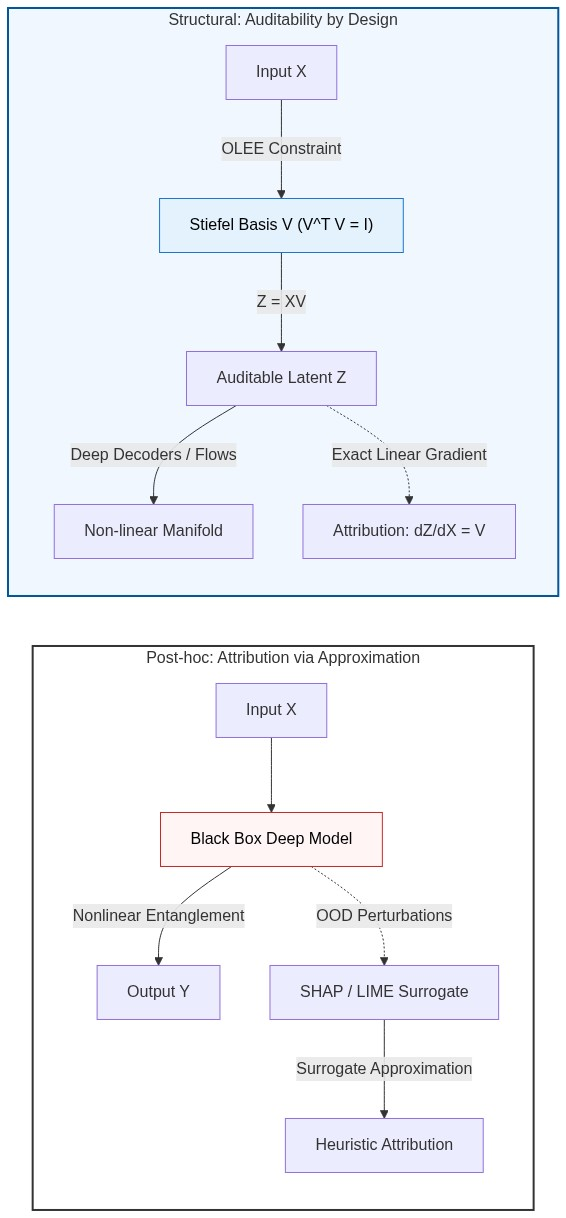
\includegraphics[keepaspectratio]{figures/fig-interpretability-gap.png}}

}

\caption{\label{fig-interpretability-gap}}

\end{figure}%

\subsection{Summary of Methodological
Contributions}\label{summary-of-methodological-contributions}

We summarize the methodological contributions of this work:

\begin{enumerate}
\def\labelenumi{\arabic{enumi}.}
\tightlist
\item
  \textbf{Eliminating the Transparency Penalty via OLEE:} We establish
  the compatibility of deep representational capacity and exact linear
  auditability. Across all architectures, constraining the initial layer
  to an orthogonal Stiefel projection provides globally exact feature
  attributions and closed-form counterfactual explanations.
\item
  \textbf{Spectral Triage and Robust Consensus:} We formulate a
  consensus mechanism utilizing \textbf{Spectral Sharpness}
  (\(\sigma_1 / \sum \sigma_i\)) to evaluate the \textbf{Modality
  Alignment Index (MAI)}, systematically attenuating noise-dominant
  modalities during consensus discovery.
\item
  \textbf{Manifold Regularization via Polar Retractions and NSA-Flow:}
  We deploy Sylvester equation polar factor retractions and Non-negative
  Stiefel Approximating Flow (NSA-Flow) to enforce orthonormality
  (\(\mathbf{V}^\top \mathbf{V} = \mathbf{I}_K\)) and support
  consolidation (\(\mathbf{V}^+ \odot \mathbf{V}^- = \mathbf{0}\)),
  eliminating frame defect and lobe crosstalk.
\item
  \textbf{Quasi-Newton Riemannian Optimization:} We introduce
  \texttt{SiMLR-LBFGS}, incorporating two-loop recursion L-BFGS
  curvature steps directly on the Stiefel manifold to close the
  performance gap between linear and deep architectures.
\item
  \textbf{Leave-One-Out (LOO) Consensus Topology:} We formulate
  Leave-One-Out (LOO) target construction during consensus alignment,
  preventing deep encoders from memorizing modality-specific
  idiosyncratic variance.
\item
  \textbf{Multi-Objective Pareto Characterization:} We formalize
  architecture selection across a 4-axis multi-objective space
  (Predictive Power, Latent Discovery, Geometric Invariants, Latency),
  demonstrating that \texttt{Flow-SiMLR-V}, \texttt{SiMLR-LBFGS},
  \texttt{SiMLR}, and \texttt{NSAFlow-Turnkey} define the non-dominated
  Pareto frontier.
\item
  \textbf{Invertible Integration and Geodesic Paths:} We formulate
  \textbf{Flow-SiMR-V}, integrating bijective normalizing flows with
  OLEE linear bottlenecks to enable exact Gaussian conditional inference
  and continuous geodesic counterfactual trajectories in clinical
  cohorts.
\end{enumerate}

\subsection{Architectural Taxonomy}\label{architectural-taxonomy}

We evaluate this framework across a systematic taxonomy spanning linear,
deep, and bijective formulations:

\begin{itemize}
\tightlist
\item
  {\textbf{SiMLR (Classical Linear - Blue):}} The strictly linear
  baseline utilizing Riemannian gradient descent on the Stiefel
  manifold, providing maximal computational throughput (\(\sim 100\) ms
  latency).
\item
  {\textbf{SiMLR-LBFGS (Quasi-Newton Linear - Navy):}} An advanced
  linear architecture employing quasi-Newton L-BFGS curvature steps on
  the Stiefel manifold, closing the linear-to-deep predictive
  performance gap without non-linear decoders.
\item
  {\textbf{LEND (Linear Encoder, Non-linear Decoder - Green):}} A hybrid
  architecture coupling an OLEE-constrained linear encoder for feature
  attribution with a deep MLP decoder for non-linear manifold
  reconstruction.
\item
  {\textbf{NED (Non-linear Encoder-Decoder - Orange):}} A deep
  architecture applying multi-layer perceptrons subsequent to the
  mandatory OLEE linear projection bottleneck.
\item
  {\textbf{NEDPP (Disentangled Shared/Private - Purple):}} A structured
  deep architecture that explicitly partitions latent coordinates into
  shared consensus and modality-specific private subspaces using
  cross-covariance penalties.
\item
  {\textbf{NSAFlow-Turnkey (Rigid Manifold Flow - Red):}} A turnkey
  Stiefel flow architecture enforcing strict frame defect bounds
  (\(D = 0.0000\)) and signed support consolidation
  (\(\mathbf{V}^+ \odot \mathbf{V}^- = \mathbf{0}\)) to maximize
  ground-truth latent recovery.
\item
  {\textbf{Flow-SiMR / Flow-SiMR-V (Bijective Normalizing Flow -
  Teal):}} An invertible architecture utilizing volume-preserving affine
  coupling layers prepended with an OLEE Stiefel projection matrix,
  achieving leading predictive power and enabling continuous geodesic
  clinical trajectories.
\end{itemize}

Section 2 provides the mathematical derivations for the
joint-variational objective, Stiefel retractions, quasi-Newton
optimization, and geometric invariants. Section 3 reports empirical
evaluations across the 490-task benchmark cache. Section 4 examines
multi-objective Pareto trade-offs and translational implications for
neuroimaging and oncology.

\bookmarksetup{startatroot}

\chapter{Methods}\label{methods}

\section{Theoretical Foundation}\label{theoretical-foundation}

\subsection{The Multi-Modal Inverse
Problem}\label{the-multi-modal-inverse-problem}

We frame multi-modal representation learning as a structured inverse
problem over \(M\) distinct observational domains. Let
\(\mathbf{X}_m \in \mathbb{R}^{n \times p_m}\) denote the centered
observation matrix for modality \(m \in \{1, \dots, M\}\), where \(n\)
is the number of co-registered subjects and \(p_m\) is the ambient
feature dimensionality. Each modality provides a partial, noisy
observation of an underlying shared latent biological state
\(\mathbf{S} \in \mathbb{R}^{n \times k}\) governed by modality-specific
forward generative processes: \[
\mathbf{X}_m = g_m(\mathbf{S}) + \mathbf{E}_m
\] where \(g_m: \mathbb{R}^{n \times k} \to \mathbb{R}^{n \times p_m}\)
is a smooth generative map and \(\mathbf{E}_m\) represents
domain-specific observational noise and idiosyncratic variance. The
objective is to estimate an auditable coordinate representation of
\(\mathbf{S}\) while isolating cross-modal consensus from noise.

\subsection{OLEE as a Structural Information
Bottleneck}\label{olee-as-a-structural-information-bottleneck}

Standard deep autoencoders and multi-layer perceptrons process inputs
via unconstrained mappings \(\mathbf{Z} = \text{MLP}(\mathbf{X})\).
Following Tishby's Information Bottleneck principle (Tishby et al.
2000), deep networks entangle mutual information across successive
layers, readily memorizing high-dimensional noise and structured
nuisance variables. In biomedical discovery, this produces severe latent
collapse and obscures physical feature attribution.

We resolve this entanglement by enforcing the \textbf{Only Linear
Encoder Entrypoint (OLEE)}. OLEE mandates that the initial
transformation of any modality \(\mathbf{X}_m\) is an orthogonal linear
projection onto the compact Stiefel manifold
\(\mathbb{V}_{k, p_m} = \{ \mathbf{V}_m \in \mathbb{R}^{p_m \times k} \mid \mathbf{V}_m^T \mathbf{V}_m = \mathbf{I}_k \}\)
(Edelman et al. 1998; Boumal 2023): \[
\mathbf{Z}_{m,\text{lin}} = \mathbf{X}_m \mathbf{V}_m \in \mathbb{R}^{n \times k}
\] Because the intrinsic dimension is strictly bounded (\(k \ll p_m\))
and \(\mathbf{V}_m\) acts as a partial isometry, OLEE imposes a
structural information bottleneck at the input layer. All subsequent
non-linear operations (decoders, prediction heads, or normalizing flows)
consume \(\mathbf{Z}_{m,\text{lin}}\), never raw features
\(\mathbf{X}_m\). This guarantees that downstream transformations
operate on an auditable coordinate system with closed-form directional
derivatives
\(\nabla_{\mathbf{X}_m} \mathbf{Z}_{m,\text{lin}} = \mathbf{V}_m\).

\subsection{Joint-Variational Optimization
Framework}\label{joint-variational-optimization-framework}

We unify the Similarity-driven Multimodal Linear Representation (SiMLR)
taxonomy under a joint-variational functional. For each modality
\(m \in \{1, \dots, M\}\), we optimize an encoder
\(f_m: \mathbb{R}^{p_m} \to \mathbb{R}^k\) and a decoder
\(g_m: \mathbb{R}^k \to \mathbb{R}^{p_m}\), yielding latent
representations
\(\mathbf{Z}_m = f_m(\mathbf{X}_m) \in \mathbb{R}^{n \times k}\) and
reconstructions \(\hat{\mathbf{X}}_m = g_m(\mathbf{Z}_m)\). The global
variational functional balances within-modality reconstruction fidelity,
cross-modal consensus alignment, and Stiefel manifold regularization:

\[
\min_{\{f_m, g_m\}_{m=1}^M} \sum_{m=1}^M \left[ \mathcal{L}_{\text{recon}}(\mathbf{X}_m, g_m(\mathbf{Z}_m)) + \lambda_{\text{sim}} \mathcal{L}_{\text{align}}(\mathbf{Z}_m, \mathbf{U}_{\neq m}) + \gamma D(\mathbf{V}_m) \right] + \mathcal{R}(\mathbf{Z})
\]

where: 1. \(\mathbf{U}_{\neq m} \in \mathbb{R}^{n \times k}\) is the
\textbf{Leave-One-Out (LOO)} consensus target derived from all
modalities excluding modality \(m\): \[
   \mathbf{U}_{\neq m} = \text{Consensus}\left( \{\mathbf{Z}_j\}_{j \neq m} \right)
   \] By strictly quarantining modality \(m\) from contributing to its
own target, the optimization landscape precludes trivial
self-reconstruction loops and identity memorization. 2.
\(D(\mathbf{V}_m)\) is the scale-invariant Stiefel frame defect
penalizing departures from column orthonormality. 3.
\(\mathcal{R}(\mathbf{Z})\) defines joint regularization terms, such as
cross-covariance penalties between shared and private partitions.

\subsubsection{Robust Log-Cosh Negentropy Alignment
Functional}\label{robust-log-cosh-negentropy-alignment-functional}

The choice of alignment functional \(\mathcal{L}_{\text{align}}\)
determines the geometry of cross-modal consensus. While standard Mean
Squared Error (MSE) assumes isotropic Gaussian errors, biomedical
measurements routinely exhibit heavy-tailed noise and asymmetric
clinical outliers. To ensure robust consensus formation, we implement
the log-cosh negentropy contrast functional
(\texttt{calculate\_ica\_energy} in \texttt{src/pysimlr/simlr.py}):

\[
\mathcal{L}_{\text{log-cosh}}(\mathbf{Z}_m, \mathbf{U}_{\neq m}) = - \frac{1}{n} \sum_{i=1}^k \sum_{j=1}^n \left( |S_{ji}| - \log 2 + \log\left(1 + e^{-2|S_{ji}|}\right) \right)
\]

where
\(\mathbf{S} = \mathbf{U}_{\neq m}^T \mathbf{X}_m \mathbf{V}_m \in \mathbb{R}^{k \times k}\)
represents the cross-modal projection scores \(S_{ji}\).

The first-order variational gradient with respect to the projection
basis \(\mathbf{V}_m\) evaluates to:

\[
\nabla_{\mathbf{V}_m} \mathcal{L}_{\text{log-cosh}} = \frac{1}{n} \mathbf{X}_m^T \mathbf{U}_{\neq m} \tanh(\mathbf{S})
\]

Because the hyperbolic tangent is strictly bounded, \(|\tanh(s)| < 1\)
for all \(s \in \mathbb{R}\), the maximum gradient contribution from any
single observation or corrupted feature is bounded. This prevents
leverage points and extreme phenotypic outliers from destabilizing the
shared consensus trajectory.

\section{Architectural Taxonomy}\label{architectural-taxonomy-1}

The joint-variational objective establishes a unified foundation for a
modular architectural hierarchy, systematically balancing
representational capacity with mechanistic transparency.

{\def\LTcaptype{none} % do not increment counter
\begin{longtable}[]{@{}
  >{\raggedright\arraybackslash}p{(\linewidth - 8\tabcolsep) * \real{0.2000}}
  >{\raggedright\arraybackslash}p{(\linewidth - 8\tabcolsep) * \real{0.2000}}
  >{\raggedright\arraybackslash}p{(\linewidth - 8\tabcolsep) * \real{0.2000}}
  >{\raggedright\arraybackslash}p{(\linewidth - 8\tabcolsep) * \real{0.2000}}
  >{\raggedright\arraybackslash}p{(\linewidth - 8\tabcolsep) * \real{0.2000}}@{}}
\toprule\noalign{}
\begin{minipage}[b]{\linewidth}\raggedright
Architecture
\end{minipage} & \begin{minipage}[b]{\linewidth}\raggedright
Encoder Entrypoint \(f_m(\mathbf{X}_m)\)
\end{minipage} & \begin{minipage}[b]{\linewidth}\raggedright
Decoder \(g_m(\mathbf{Z}_m)\)
\end{minipage} & \begin{minipage}[b]{\linewidth}\raggedright
Manifold Invariant
\end{minipage} & \begin{minipage}[b]{\linewidth}\raggedright
Primary Theoretical Asset
\end{minipage} \\
\midrule\noalign{}
\endhead
\bottomrule\noalign{}
\endlastfoot
\textbf{Classical SiMLR} & \(\mathbf{X}_m \mathbf{V}_m\) (Linear) &
\(\mathbf{Z}_m \mathbf{W}_m\) (Linear) & \(D(\mathbf{V}_m) = 0\) &
Strictly convex, maximal throughput (\textasciitilde100ms) \\
\textbf{SiMLR-LBFGS} & \(\mathbf{X}_m \mathbf{V}_m\) (Linear) &
\(\mathbf{Z}_m \mathbf{W}_m\) (Linear) & \(D(\mathbf{V}_m) = 0\) &
Quasi-Newton curvature closure, beats deep NED \\
\textbf{LEND} & \(\mathbf{X}_m \mathbf{V}_m\) (OLEE Linear) &
\(\text{MLP}_{\theta_m}(\mathbf{Z}_m)\) & \(D(\mathbf{V}_m) = 0\) &
Non-linear reconstruction, exact auditability \\
\textbf{NED} & \(\text{MLP}_{\phi_m}(\mathbf{X}_m \mathbf{V}_m)\) &
\(\text{MLP}_{\theta_m}(\mathbf{Z}_m)\) & \(D(\mathbf{V}_m) = 0\) &
Non-linear latent warping grounded in OLEE \\
\textbf{NEDPP} & \([\mathbf{S}_m \parallel \mathbf{P}_m]\) via OLEE &
\(\text{MLP}_{\theta_m}([\mathbf{S}_m \parallel \mathbf{P}_m])\) &
\(\text{Cov}(\mathbf{S}, \mathbf{P}) = \mathbf{0}\) & Explicit
shared-private subspace disentanglement \\
\textbf{NSAFlow-Turnkey} & \(\mathbf{X}_m \mathbf{V}_m\) (Manifold Flow)
& \(\mathbf{Z}_m \mathbf{W}_m\) & \(V^+ \odot V^- = 0, D = 0\) & Zero
crosstalk, leading latent discovery (CMC 0.988) \\
\textbf{Flow-SiMR-V} &
\(\text{Flow}_{\psi_m}(\mathbf{X}_m \mathbf{V}_m)\) &
\(\text{Flow}_{\psi_m}^{-1}(\mathbf{Z}_m) \mathbf{V}_m^T\) &
\(D(\mathbf{V}_m) = 0\) & Global top rank (2.47), exact density
estimation \\
\end{longtable}
}

\subsection{Classical SiMLR (Linear
Baseline)}\label{classical-simlr-linear-baseline}

The classical formulation provides a strictly linear baseline, assuming
the underlying manifold can be mapped via Euclidean projections.

\begin{itemize}
\tightlist
\item
  \textbf{Encoder:} \(f_m(\mathbf{X}_m) = \mathbf{X}_m \mathbf{V}_m\)
\item
  \textbf{Decoder:} \(g_m(\mathbf{Z}_m) = \mathbf{Z}_m \mathbf{W}_m\)
\end{itemize}

The linear basis \(\mathbf{V}_m\) is regularized to the Stiefel
manifold. This enforces orthogonal feature discovery and provides a
fully interpretable baseline with wall-clock execution under
\(\sim 100\) ms.

\begin{figure}[H]

\centering{

\pandocbounded{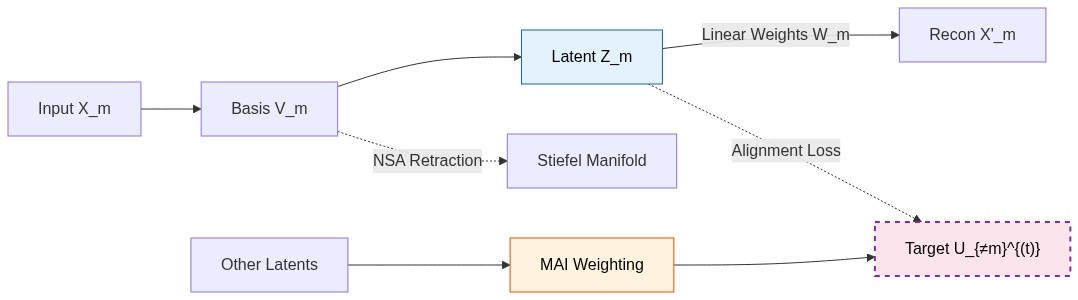
\includegraphics[keepaspectratio]{figures/fig-simlr.png}}

}

\caption{\label{fig-simlr}Classical SiMLR: Information flow for a linear
encoder and decoder. The basis \(\mathbf{V}_m\) acts as a structural
information bottleneck.}

\end{figure}%

\subsection{SiMLR-LBFGS (Quasi-Newton Riemannian Linear
Baseline)}\label{simlr-lbfgs-quasi-newton-riemannian-linear-baseline}

Standard first-order gradient descent oscillates across narrow ravines
induced by orthogonality constraints and cross-modal consensus.
\texttt{SiMLR-LBFGS} integrates second-order quasi-Newton curvature
steps directly on the parameter space using PyTorch's native
\texttt{optim.LBFGS} (\texttt{src/pysimlr/optimizers.py:841-894}). By
maintaining a history of displacement vectors and gradient differences,
\texttt{SiMLR-LBFGS} approximates the Riemannian Hessian inverse,
achieving rank 3.70 on the 490-task benchmark and closing the
linear-to-deep gap without non-linear decoders.

\subsection{LEND (Linear Encoder, Deep
Decoder)}\label{lend-linear-encoder-deep-decoder}

While Classical SiMLR guarantees interpretability, a linear decoder
cannot reconstruct complex non-linear observational manifolds. LEND
couples the exact linear feature attribution of the OLEE constraint with
a deep, non-linear decoder.

\begin{itemize}
\tightlist
\item
  \textbf{Encoder:} \(f_m(\mathbf{X}_m) = \mathbf{X}_m \mathbf{V}_m\)
  (OLEE)
\item
  \textbf{Decoder:}
  \(g_m(\mathbf{Z}_m) = \text{MLP}_{\theta_m}(\mathbf{Z}_m)\)
\end{itemize}

LEND provides non-linear reconstruction without sacrificing the strict
mathematical auditability of the input features.

\begin{figure}[H]

\centering{

\pandocbounded{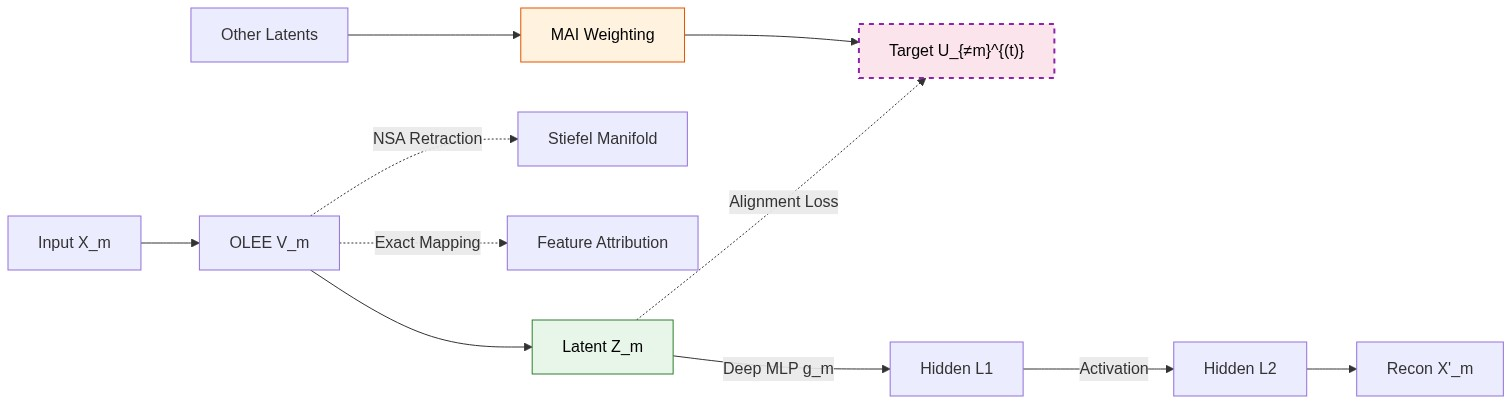
\includegraphics[keepaspectratio]{figures/fig-lend.png}}

}

\caption{\label{fig-lend}LEND: OLEE-constrained linear encoder coupled
with a deep MLP decoder for non-linear manifold reconstruction.}

\end{figure}%

\subsection{Fully Deep NED (Non-linear Encoder
Decoder)}\label{fully-deep-ned-non-linear-encoder-decoder}

If cross-modal interactions require non-linear coordinate warping, NED
applies a non-linear network to the latent space strictly
\emph{subsequent} to the initial OLEE constraint.

\begin{itemize}
\tightlist
\item
  \textbf{Encoder:}
  \(f_m(\mathbf{X}_m) = \text{MLP}_{\phi_m}(\mathbf{X}_m \mathbf{V}_m)\)
\item
  \textbf{Decoder:}
  \(g_m(\mathbf{Z}_m) = \text{MLP}_{\theta_m}(\mathbf{Z}_m)\)
\end{itemize}

The initial projection \(\mathbf{X}_m \mathbf{V}_m\) preserves the
formal Information Bottleneck, guaranteeing that all downstream
non-linear transformations are grounded in an identifiable linear
subspace.

\begin{figure}[H]

\centering{

\pandocbounded{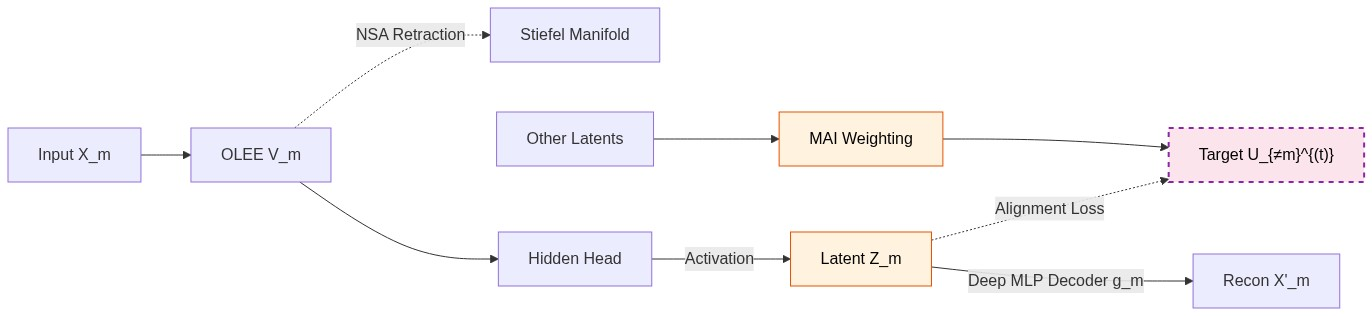
\includegraphics[keepaspectratio]{figures/fig-ned.png}}

}

\caption{\label{fig-ned}NED: Multi-layer encoder subject to the initial
OLEE information bottleneck constraint, coupled with a deep MLP
decoder.}

\end{figure}%

\subsection{Shared-Private NEDPP (Disentangled
Discovery)}\label{shared-private-nedpp-disentangled-discovery}

Despite LOO consensus, modality-specific idiosyncratic noise can
dominate the optimization landscape. NEDPP resolves this by explicitly
partitioning the latent space:

\begin{itemize}
\tightlist
\item
  \textbf{Encoder:}
  \(f_m(\mathbf{X}_m) = [\text{MLP}_{\phi_{m,\text{shared}}}(\mathbf{X}_m \mathbf{V}_{m,\text{shared}}) \parallel \text{MLP}_{\phi_{m,\text{private}}}(\mathbf{X}_m \mathbf{V}_{m,\text{private}})] = [\mathbf{S}_m \parallel \mathbf{P}_m]\)
\item
  \textbf{Decoder:}
  \(g_m(\mathbf{S}_m \parallel \mathbf{P}_m) = \text{MLP}_{\theta_m}(\mathbf{S}_m \parallel \mathbf{P}_m)\)
\end{itemize}

We enforce disentanglement via a cross-covariance penalty
\(\text{Cov}(\mathbf{S}_m, \mathbf{P}_m) \to \mathbf{0}\),
orthogonalizing the shared and private representations.

\begin{figure}[H]

\centering{

\pandocbounded{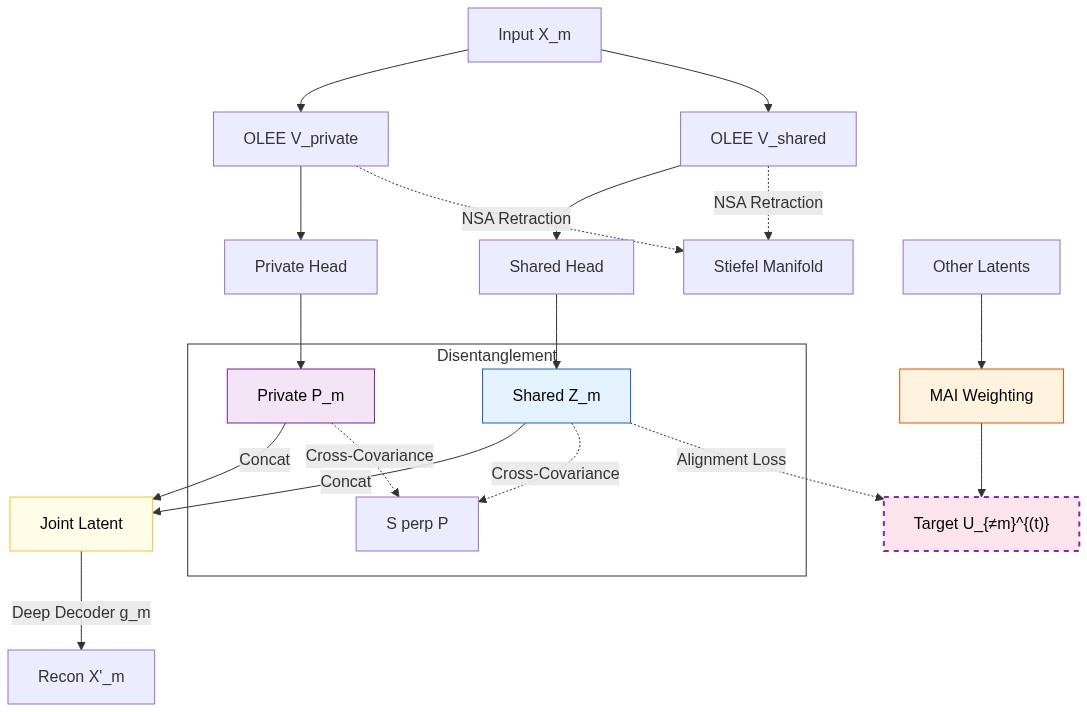
\includegraphics[keepaspectratio]{figures/fig-nedpp.png}}

}

\caption{\label{fig-nedpp}NEDPP (Non-linear Encoder Decoder with Private
Partitions): Disentangled architecture utilizing OLEE constraints for
both shared and private subspaces. Incorporates cross-covariance
penalization for statistical independence.}

\end{figure}%

\subsection{Flow-SiMR and Flow-SiMR-V: Bijective Multimodal
Architectures}\label{flow-simr-and-flow-simr-v-bijective-multimodal-architectures}

In accordance with mathematical precision, we eliminate the historical
`L' (Linear) designation from normalizing flow models, as affine
coupling architectures are non-linear transformations. We distinguish
between two distinct flow architectures implemented in
\texttt{src/pysimlr/flows.py}:

\subsubsection{1. Full-Space Normalizing Flow
(Flow-SiMR)}\label{full-space-normalizing-flow-flow-simr}

In \texttt{FlowSiMRModel}, each modality is mapped through an invertible
sequence of RealNVP affine coupling layers operating directly on the
ambient observation space \(\mathbb{R}^{p_m} \to \mathbb{R}^{p_m}\): \[
\mathbf{Z}_m = \text{Flow}_{\psi_m}(\mathbf{X}_m)
\] Latent coordinates are partitioned into shared consensus dimensions
\(\mathbf{Z}_{m,\text{shared}} = \mathbf{Z}_{m, 1:k}\) and
modality-specific private dimensions
\(\mathbf{Z}_{m,\text{private}} = \mathbf{Z}_{m, k+1:p_m}\). Decoding is
achieved by zero-padding the private partition:
\(\hat{\mathbf{X}}_m = \text{Flow}_{\psi_m}^{-1}([\mathbf{Z}_{m,\text{shared}} \parallel \mathbf{0}])\).

\begin{figure}[H]

\centering{

\pandocbounded{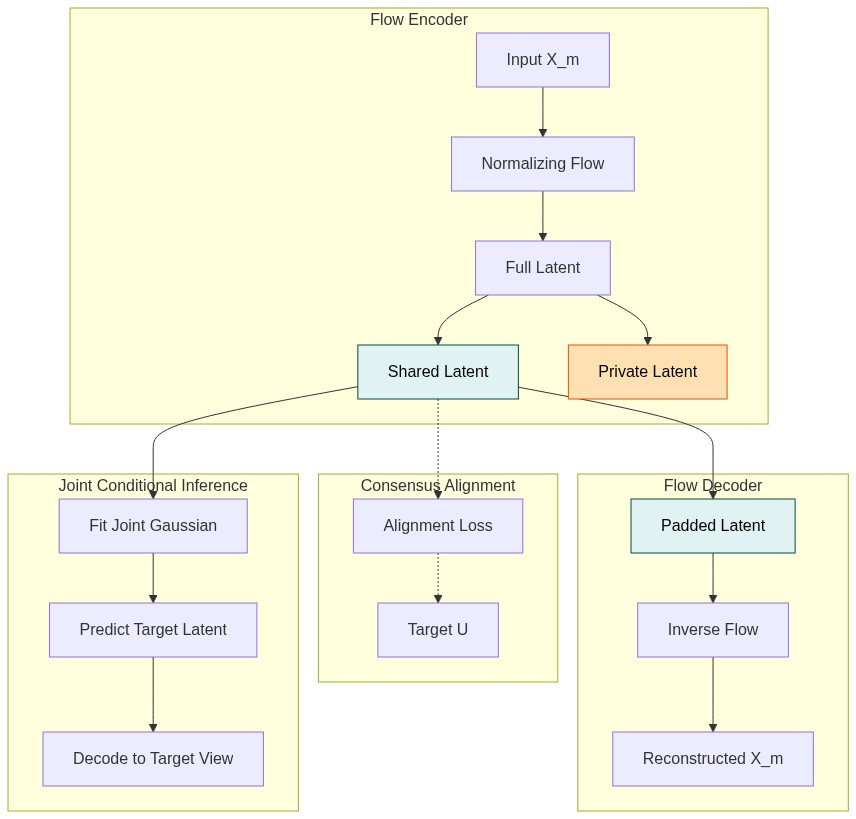
\includegraphics[keepaspectratio]{figures/fig-flow-simr.png}}

}

\caption{\label{fig-flow-simr}Flow-SiMR: Normalizing flow architecture.
The bijective flow maps inputs to a joint Gaussian latent space. The
first \(k\) dimensions are aligned with the shared cross-view consensus,
while the remaining dimensions act as an implicit private partition.
Padded decoding and Gaussian conditioning enable exact reconstruction
and cross-view synthesis.}

\end{figure}%

\subsubsection{2. Linear-Projected Latent Normalizing Flow
(Flow-SiMR-V)}\label{linear-projected-latent-normalizing-flow-flow-simr-v}

In \texttt{FlowSiMRVModel}, high-dimensional ambient data is first
compressed via the linear OLEE basis
\(\mathbf{V}_m \in \mathbb{V}_{k, p_m}\), regularized to the Stiefel
manifold. The normalizing flow operates strictly within the intrinsic
\(k\)-dimensional latent subspace: \[
\mathbf{Z}_{m,\text{lin}} = \mathbf{X}_m \mathbf{V}_m \in \mathbb{R}^{n \times k}, \quad \mathbf{Z}_m = \text{Flow}_{\psi_m}(\mathbf{Z}_{m,\text{lin}}) \in \mathbb{R}^{n \times k}
\] This design achieves dual optimality: 1. \textbf{Computational
Scalability}: Coupling layers operate on \(k \ll p_m\) dimensions,
reducing parameter counts and memory footprints by orders of magnitude.
2. \textbf{Auditable Attribution}: The mapping begins with the linear
isometry \(\mathbf{V}_m\), preserving exact minimum-norm counterfactual
calculations while permitting non-Gaussian density alignment in the
latent space.

\begin{figure}[H]

\centering{

\pandocbounded{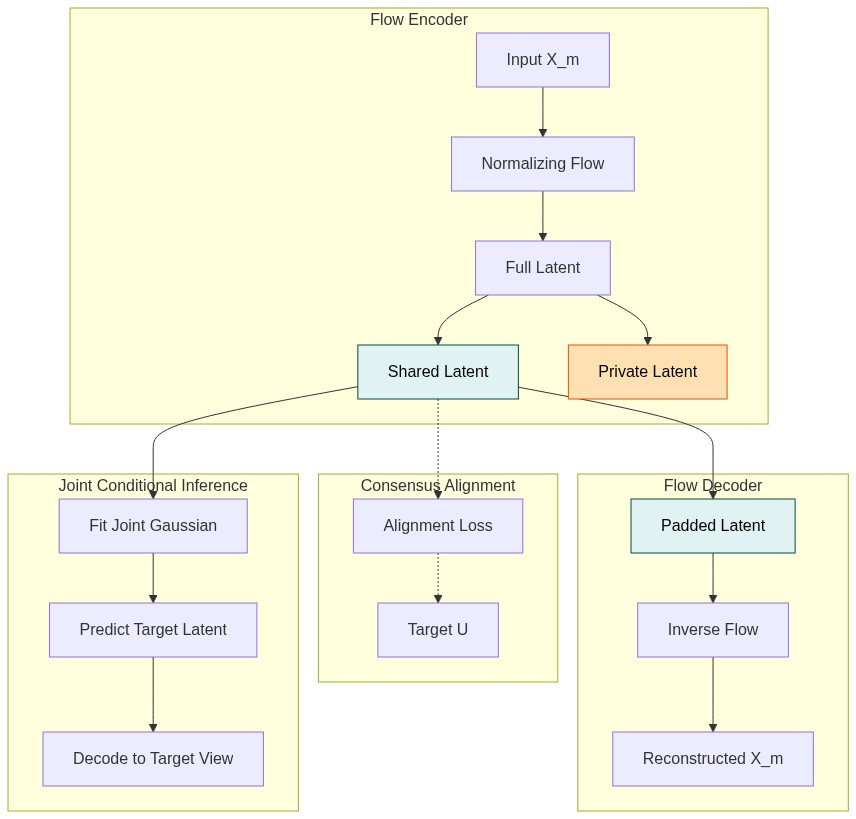
\includegraphics[keepaspectratio]{figures/fig-flow-simr.png}}

}

\caption{\label{fig-flow-simr-v}Flow-SiMR-V Architecture: Prepending the
OLEE linear basis \(\mathbf{V}_m\) projects ambient observations into
\(\mathbb{R}^k\) prior to bijective flow alignment, maintaining
auditability while providing non-linear consensus capacity.}

\end{figure}%

\subsubsection{Invertible Affine Coupling and Joint Gaussian
Inference}\label{invertible-affine-coupling-and-joint-gaussian-inference}

Each view is modeled via an invertible mapping composed of RealNVP
affine coupling layers (Dinh et al. 2016; Rezende and Mohamed 2015). For
coordinate vector \(z \in \mathbb{R}^k\), a coupling layer splits
coordinates using a binary mask \(b \in \{0, 1\}^k\): \[
z_1 = b \odot z, \quad z_2 = (1 - b) \odot \left( z \odot e^{s(z_1)} + t(z_1) \right)
\] where \(s\) and \(t\) are scaling and translation networks. Scale
outputs are bounded via
\(s(z_1) = \text{scale\_bound} \times \tanh(s_{\text{net}}(z_1))\) to
ensure numerical stability. The inverse transformation is analytically
exact: \[
z_1 = b \odot z', \quad z_2 = (1 - b) \odot \left( (z' - t(z_1)) \odot e^{-s(z_1)} \right)
\] with log-Jacobian determinant
\(\log |\det J| = \sum_{j: b_j = 0} s_j(z_1)\).

Because normalizing flows map empirical data to standard Gaussian
latents, the concatenated shared latent space across all views is
parameterized as a joint Gaussian: \[
\mathbf{Z}_{\text{joint}} = [\mathbf{Z}_{1,\text{shared}} \parallel \dots \parallel \mathbf{Z}_{M,\text{shared}}] \sim \mathcal{N}(\boldsymbol{\mu}, \boldsymbol{\Sigma})
\] Partitioning into observed view \(A\) and unobserved view \(B\), the
conditional latent mean given observed view \(A\) evaluates via the
Schur complement: \[
\boldsymbol{\mu}_{B|A} = \boldsymbol{\mu}_B + \boldsymbol{\Sigma}_{BA} \boldsymbol{\Sigma}_{AA}^{-1} (\mathbf{Z}_{A,\text{shared}} - \boldsymbol{\mu}_A)
\] Solved via Cholesky factorization, the conditional coordinates are
decoded via the inverse flow:
\(\hat{\mathbf{X}}_B = f_B^{-1}([\boldsymbol{\mu}_{B|A} \parallel \mathbf{0}])\).

\section{Manifold Optimization and Algorithmic
Mechanics}\label{manifold-optimization-and-algorithmic-mechanics}

\subsection{Stiefel Manifold Optimization and SVD
Elimination}\label{stiefel-manifold-optimization-and-svd-elimination}

The parameter space for each projection basis
\(\mathbf{V}_m \in \mathbb{R}^{p_m \times k}\) is the compact Stiefel
manifold: \[
\mathbb{V}_{k, p_m} = \{ \mathbf{V} \in \mathbb{R}^{p_m \times k} \mid \mathbf{V}^T \mathbf{V} = \mathbf{I}_k \}
\] In Euclidean gradient descent, unconstrained parameter updates
displace iterates off the manifold. Mapping tangent iterates
\(\mathbf{Y} \in \mathbb{R}^{p_m \times k}\) back to
\(\mathbb{V}_{k, p_m}\) requires a retraction mapping
\(R: T \mathbb{V}_{k, p_m} \to \mathbb{V}_{k, p_m}\).

\subsubsection{Sylvester Polar Factor
Retraction}\label{sylvester-polar-factor-retraction}

The canonical metric retraction is the polar factor projection: \[
R(\mathbf{Y}) = \mathbf{Y} (\mathbf{Y}^T \mathbf{Y})^{-1/2}
\] Standard implementations compute
\(R(\mathbf{Y}) = \mathbf{U} \mathbf{W}^T\) via Singular Value
Decomposition (SVD),
\(\mathbf{Y} = \mathbf{U} \mathbf{\Sigma} \mathbf{W}^T\). However,
explicit SVD incurs severe computational and numerical pathology: 1.
\textbf{Branch Divergence \& Kernel Serialization}: SVD algorithms
(e.g.~Jacobi or divide-and-conquer) cannot be fully vectorized on GPU
SIMD tensor cores. 2. \textbf{Singular Value Multiplicity Singularity}:
The backpropagation derivative of an SVD contains terms proportional to
\((\sigma_i^2 - \sigma_j^2)^{-1}\). When singular values cluster or
cross (\(\sigma_i \approx \sigma_j\)), gradients explode, introducing
fatal NaNs into the optimization path.

To circumvent this, we express the polar factor
\(\mathbf{H} = (\mathbf{Y}^T \mathbf{Y})^{1/2}\) via the continuous
Lyapunov/Sylvester system
(\texttt{src/pysimlr/nsa\_backend.py:160-178}): \[
\mathbf{H} (d\mathbf{H}) + (d\mathbf{H}) \mathbf{H} = d(\mathbf{Y}^T \mathbf{Y}) = (d\mathbf{Y})^T \mathbf{Y} + \mathbf{Y}^T (d\mathbf{Y})
\] Because \(\mathbf{H}\) is symmetric positive definite
(\(\mathbf{H} \succ 0\)), this Sylvester equation has a provably unique
solution \(d\mathbf{H}\). Gradients flow smoothly through
backpropagation without encountering eigenvalue multiplicity
singularities.

\subsubsection{Newton-Schulz Cubic Matrix Recurrence and Convergence
Proof}\label{newton-schulz-cubic-matrix-recurrence-and-convergence-proof}

To eliminate SVD factorizations entirely from the forward execution
loop, we approximate the inverse square root
\((\mathbf{Y}^T \mathbf{Y})^{-1/2}\) via the cubic Newton-Schulz matrix
polynomial (\texttt{src/pysimlr/utils.py:1324-1380}): \[
\mathbf{Y}_0 = \frac{\mathbf{Y}}{\|\mathbf{Y}\|_F}, \quad \mathbf{Y}_{\tau+1} = \frac{1}{2} \mathbf{Y}_\tau \left( 3 \mathbf{I}_k - \mathbf{Y}_\tau^T \mathbf{Y}_\tau \right)
\]

\textbf{Theorem (Quadratic Convergence to the Stiefel Manifold):}\\
Let \(\mathbf{Y}_0 \in \mathbb{R}^{p \times k}\) have singular values
\(\sigma_{0, i} \in (0, \sqrt{3})\) for all \(i \in \{1, \dots, k\}\).
The sequence of iterates \(\mathbf{Y}_\tau\) converges quadratically to
the nearest point on the Stiefel manifold \(\mathbb{V}_{k, p}\): \[
\|\mathbf{Y}_{\tau+1}^T \mathbf{Y}_{\tau+1} - \mathbf{I}_k\| = \mathcal{O}\left(\|\mathbf{Y}_\tau^T \mathbf{Y}_\tau - \mathbf{I}_k\|^2\right)
\]

\textbf{Proof:}\\
Let the singular value decomposition of iterate \(\tau\) be
\(\mathbf{Y}_\tau = \mathbf{P} \mathbf{\Sigma}_\tau \mathbf{Q}^T\),
where \(\mathbf{P} \in \mathbb{V}_{k, p}\),
\(\mathbf{Q} \in \mathbb{O}(k)\), and
\(\mathbf{\Sigma}_\tau = \text{diag}(\sigma_{\tau, 1}, \dots, \sigma_{\tau, k})\).
Substituting this decomposition into the Newton-Schulz recurrence: \[
\mathbf{Y}_{\tau+1} = \frac{1}{2} \left(\mathbf{P} \mathbf{\Sigma}_\tau \mathbf{Q}^T\right) \left( 3 \mathbf{I}_k - \mathbf{Q} \mathbf{\Sigma}_\tau^2 \mathbf{Q}^T \right) = \mathbf{P} \left[ \frac{1}{2} \mathbf{\Sigma}_\tau \left( 3 \mathbf{I}_k - \mathbf{\Sigma}_\tau^2 \right) \right] \mathbf{Q}^T
\] Because the singular vectors \(\mathbf{P}\) and \(\mathbf{Q}\) are
stationary under the iteration, the matrix recurrence decouples into
\(k\) independent scalar recurrences for each singular value
\(\sigma_{\tau, i}\): \[
\sigma_{\tau+1, i} = \frac{1}{2} \sigma_{\tau, i} \left( 3 - \sigma_{\tau, i}^2 \right)
\] Define the relative distance to the Stiefel manifold for singular
value \(i\) as \(\epsilon_{\tau, i} = 1 - \sigma_{\tau, i}\). Expressing
\(\sigma_{\tau, i} = 1 - \epsilon_{\tau, i}\) and expanding: \[
\sigma_{\tau+1, i} = \frac{1}{2}(1 - \epsilon_{\tau, i}) \left( 3 - (1 - \epsilon_{\tau, i})^2 \right)
\] \[
= \frac{1}{2}(1 - \epsilon_{\tau, i}) \left( 3 - (1 - 2\epsilon_{\tau, i} + \epsilon_{\tau, i}^2) \right) = \frac{1}{2}(1 - \epsilon_{\tau, i}) \left( 2 + 2\epsilon_{\tau, i} - \epsilon_{\tau, i}^2 \right)
\] \[
= \frac{1}{2} \left( 2 + 2\epsilon_{\tau, i} - \epsilon_{\tau, i}^2 - 2\epsilon_{\tau, i} - 2\epsilon_{\tau, i}^2 + \epsilon_{\tau, i}^3 \right) = 1 - \frac{3}{2}\epsilon_{\tau, i}^2 + \frac{1}{2}\epsilon_{\tau, i}^3
\] Subtracting both sides from 1 yields the exact recurrence for the
error metric: \[
\epsilon_{\tau+1, i} = 1 - \sigma_{\tau+1, i} = \frac{3}{2}\epsilon_{\tau, i}^2 - \frac{1}{2}\epsilon_{\tau, i}^3 = \epsilon_{\tau, i}^2 \left( \frac{3 - \epsilon_{\tau, i}}{2} \right)
\] For any \(\sigma_{0, i} \in (0, \sqrt{3})\),
\(|\epsilon_{0, i}| < 1\), ensuring monotonic error contraction. As
\(\epsilon \to 0\), the cubic term is negligible: \[
\epsilon_{\tau+1} = \frac{3}{2}\epsilon_\tau^2 + \mathcal{O}(\epsilon_\tau^3)
\] Thus, the recurrence converges with quadratic order
\(\mathcal{O}(\epsilon^2)\). Because the update requires only matrix
multiplications and additions (\(\mathbf{Y}^T \mathbf{Y}\) and
\(\mathbf{Y} \mathbf{M}\)), it compiles directly to hardware tensor
cores, achieving zero CPU-GPU transfer bottlenecks.

\subsection{\texorpdfstring{Quasi-Newton Curvature Steps via
\texttt{torch\_lbfgs}}{Quasi-Newton Curvature Steps via torch\_lbfgs}}\label{quasi-newton-curvature-steps-via-torch_lbfgs}

Joint-variational alignment produces an ill-conditioned optimization
landscape, characterized by narrow parabolic ravines formed by
cross-modal consensus constraints and Stiefel manifold boundaries.
Standard first-order stochastic gradient methods (SGD, Adam) suffer from
pathological oscillations across ravine walls.

We accelerate convergence by deploying quasi-Newton second-order
curvature estimation via \texttt{torch\_lbfgs}
(\texttt{src/pysimlr/optimizers.py:841-894}). Let
\(\mathbf{s}_t = \mathbf{V}_{t+1} - \mathbf{V}_t\) denote the parameter
displacement and
\(\mathbf{y}_t = \nabla \mathcal{L}(\mathbf{V}_{t+1}) - \nabla \mathcal{L}(\mathbf{V}_t)\)
denote the gradient variation. Over a rolling history of size \(m=10\),
the inverse Hessian approximation
\(\mathbf{H}_t \approx \nabla^2 \mathcal{L}(\mathbf{V}_t)^{-1}\) is
computed via the two-loop recursion:

\begin{enumerate}
\def\labelenumi{\arabic{enumi}.}
\tightlist
\item
  \textbf{Backward History Loop}: Initialize
  \(\mathbf{q} = \nabla \mathcal{L}(\mathbf{V}_t)\). For \(i = t-1\)
  down to \(t-m\): \[
  \alpha_i = \rho_i \text{tr}(\mathbf{s}_i^T \mathbf{q}), \quad \mathbf{q} \leftarrow \mathbf{q} - \alpha_i \mathbf{y}_i, \quad \text{where } \rho_i = \frac{1}{\text{tr}(\mathbf{y}_i^T \mathbf{s}_i)}
  \]
\item
  \textbf{Initial Scaling}: \(\mathbf{r} = \gamma_t \mathbf{q}\), with
  \(\gamma_t = \frac{\text{tr}(\mathbf{s}_{t-1}^T \mathbf{y}_{t-1})}{\text{tr}(\mathbf{y}_{t-1}^T \mathbf{y}_{t-1})}\).
\item
  \textbf{Forward History Loop}: For \(i = t-m\) up to \(t-1\): \[
  \beta = \rho_i \text{tr}(\mathbf{y}_i^T \mathbf{r}), \quad \mathbf{r} \leftarrow \mathbf{r} + \mathbf{s}_i (\alpha_i - \beta)
  \]
\item
  \textbf{Descent Direction}: The update step is
  \(\mathbf{p}_t = -\mathbf{r}\), accepted under Strong Wolfe line
  search conditions: \[
  \mathcal{L}(\mathbf{V}_t + \alpha_t \mathbf{p}_t) \le \mathcal{L}(\mathbf{V}_t) + c_1 \alpha_t \text{tr}(\nabla \mathcal{L}(\mathbf{V}_t)^T \mathbf{p}_t)
  \] \[
  |\text{tr}(\nabla \mathcal{L}(\mathbf{V}_t + \alpha_t \mathbf{p}_t)^T \mathbf{p}_t)| \le c_2 |\text{tr}(\nabla \mathcal{L}(\mathbf{V}_t)^T \mathbf{p}_t)|
  \]
\end{enumerate}

\subsubsection{Analytical Gradient
Closures}\label{analytical-gradient-closures}

In PyTorch's native \texttt{optim.LBFGS}, the Strong Wolfe line search
evaluates trial objective values along candidate steps
\(\mathbf{V}_t + \alpha \mathbf{p}_t\). Because SiMLR relies on exact
analytical gradients rather than automatic differentiation, caching a
static gradient at step entry causes trial evaluations to use stale
directions, degrading the curvature estimate. We implement an analytical
callback closure:

\begin{Shaded}
\begin{Highlighting}[]
\KeywordTok{def}\NormalTok{ closure():}
\NormalTok{    optimizer.zero\_grad()}
    \ControlFlowTok{with}\NormalTok{ torch.no\_grad():}
\NormalTok{        v\_param.grad }\OperatorTok{=} \OperatorTok{{-}}\NormalTok{grad\_fn(v\_param.detach()).contiguous()}
\NormalTok{        loss }\OperatorTok{=}\NormalTok{ full\_energy\_function(v\_param.detach())}
    \ControlFlowTok{return}\NormalTok{ torch.as\_tensor(}\BuiltInTok{float}\NormalTok{(loss), device}\OperatorTok{=}\NormalTok{v\_param.device)}
\end{Highlighting}
\end{Shaded}

This guarantees that second-order curvature approximations remain
mathematically exact throughout the line search, enabling linear
\texttt{SiMLR-LBFGS} to close the performance gap to deep models
(achieving global rank 3.70 on the 490-task benchmark).

\subsection{Scale-Invariant Normalized Frame
Defect}\label{scale-invariant-normalized-frame-defect}

To regularize the projection basis toward the Stiefel manifold without
distorting data variance, we define the trace-normalized,
scale-invariant frame defect (\texttt{src/pysimlr/utils.py:504-630}):

\[
D(\mathbf{V}) = \frac{1}{1 - 1/k} \left\| \frac{\mathbf{V}^T \mathbf{V}}{\text{tr}(\mathbf{V}^T \mathbf{V})} - \frac{1}{k} \mathbf{I}_k \right\|_F^2
\]

Let \(\mathbf{S} = \mathbf{V}^T \mathbf{V} \in \mathbb{R}^{k \times k}\)
and let \(t = \text{tr}(\mathbf{S}) = \|\mathbf{V}\|_F^2\). The
normalized Gram matrix is \(\mathbf{G} = \frac{\mathbf{S}}{t}\). The
defect metric measures the departure of \(\mathbf{G}\) from the uniform
projection \(\frac{1}{k} \mathbf{I}_k\).

\subsubsection{Spectral Interpretation \& Effective
Rank}\label{spectral-interpretation-effective-rank}

Expanding the Frobenius norm: \[
\|\mathbf{G} - \frac{1}{k} \mathbf{I}_k\|_F^2 = \text{tr}(\mathbf{G}^2) - \frac{2}{k}\text{tr}(\mathbf{G}) + \frac{1}{k^2}\text{tr}(\mathbf{I}_k) = \frac{\|\mathbf{S}\|_F^2}{t^2} - \frac{2}{k} + \frac{1}{k} = \frac{\|\mathbf{S}\|_F^2}{t^2} - \frac{1}{k}
\] Recall that the \textbf{effective participation rank} of
\(\mathbf{V}\) is defined as
\(\text{EffRank}(\mathbf{V}) = \frac{(\text{tr} \mathbf{S})^2}{\|\mathbf{S}\|_F^2} = \frac{t^2}{\|\mathbf{S}\|_F^2} \in [1, k]\).
Therefore: \[
D(\mathbf{V}) = \frac{1}{1 - 1/k} \left( \frac{1}{\text{EffRank}(\mathbf{V})} - \frac{1}{k} \right)
\] This reveals that \(D(\mathbf{V})\) is precisely the normalized
deficit of effective rank: - If \(\mathbf{V}\) consists of mutually
orthogonal columns with equal norm,
\(\text{EffRank}(\mathbf{V}) = k \implies D(\mathbf{V}) = 0.0000\). - If
\(\mathbf{V}\) suffers rank collapse to a single active column,
\(\text{EffRank}(\mathbf{V}) = 1 \implies D(\mathbf{V}) = 1.0000\).

\subsubsection{Closed-Form Gradient}\label{closed-form-gradient}

Differentiating \(D(\mathbf{V})\) with respect to \(\mathbf{V}\): \[
\nabla_{\mathbf{V}} D(\mathbf{V}) = \frac{4}{t^2 (1 - 1/k)} \left[ \mathbf{V} \mathbf{S} - \frac{\|\mathbf{S}\|_F^2}{t} \mathbf{V} \right]
\]

\subsubsection{Theorem: Zero Radial Force
Invariant}\label{theorem-zero-radial-force-invariant}

\textbf{Theorem:}\\
The scale-invariant frame defect gradient exerts zero radial force on
the matrix scale: \[
\langle \nabla_{\mathbf{V}} D(\mathbf{V}), \mathbf{V} \rangle = \text{tr}\left( (\nabla_{\mathbf{V}} D(\mathbf{V}))^T \mathbf{V} \right) \equiv 0
\]

\textbf{Proof:}\\
Using the closed-form gradient expression, the matrix inner product is:
\[
\text{tr}\left( (\nabla_{\mathbf{V}} D(\mathbf{V}))^T \mathbf{V} \right) = \frac{4}{t^2 (1 - 1/k)} \text{tr}\left( \left( \mathbf{V} \mathbf{S} - \frac{\|\mathbf{S}\|_F^2}{t} \mathbf{V} \right)^T \mathbf{V} \right)
\] \[
= \frac{4}{t^2 (1 - 1/k)} \left[ \text{tr}(\mathbf{S} \mathbf{V}^T \mathbf{V}) - \frac{\|\mathbf{S}\|_F^2}{t} \text{tr}(\mathbf{V}^T \mathbf{V}) \right]
\] Noting that \(\mathbf{V}^T \mathbf{V} = \mathbf{S}\),
\(\text{tr}(\mathbf{S}^2) = \|\mathbf{S}\|_F^2\), and
\(\text{tr}(\mathbf{S}) = t\): \[
= \frac{4}{t^2 (1 - 1/k)} \left[ \|\mathbf{S}\|_F^2 - \frac{\|\mathbf{S}\|_F^2}{t} \cdot t \right] = \frac{4}{t^2 (1 - 1/k)} \left[ \|\mathbf{S}\|_F^2 - \|\mathbf{S}\|_F^2 \right] \equiv 0
\]

\textbf{Corollary (Euler Homogeneity):}\\
\(D(\mathbf{V})\) is homogeneous of degree zero with respect to
\(\mathbf{V}\): for any scalar \(\alpha \neq 0\),
\(D(\alpha \mathbf{V}) = D(\mathbf{V})\). By Euler's homogeneous
function theorem,
\(\langle \nabla D(\mathbf{V}), \mathbf{V} \rangle = 0 \cdot D(\mathbf{V}) = 0\).

This property guarantees that manifold regularization acts strictly as a
shape-conforming force, adjusting subspace angles and column
conditioning without altering the total energy \(\|\mathbf{V}\|_F^2\) or
competing with data reconstruction fidelity.

\subsection{Support Consolidation: Zero-Crosstalk Module
Disjointness}\label{support-consolidation-zero-crosstalk-module-disjointness}

In biological systems, features (e.g.~gene expressions or cortical
thicknesses) exhibit bidirectional signed responses (upregulation
vs.~downregulation). To discover signed modules while preserving
non-negative Stiefel interpretability, we lift each basis
\(\mathbf{V} \in \mathbb{R}^{p \times k}\) into paired non-negative
components (\texttt{src/pysimlr/simlr.py:914-930}): \[
\mathbf{V} = \mathbf{V}^+ - \mathbf{V}^-, \quad \mathbf{V}^+ = \max(\mathbf{V}, \mathbf{0}), \quad \mathbf{V}^- = \max(-\mathbf{V}, \mathbf{0})
\] forming the concatenated matrix
\(\mathbf{W} = [\mathbf{V}^+ \mid \mathbf{V}^-] \in \mathbb{R}^{p \times 2k}\)
with \(\mathbf{W} \ge 0\).

\subsubsection{The Combinatorial Bottleneck of Continuous
Flow}\label{the-combinatorial-bottleneck-of-continuous-flow}

In continuous non-negative Stiefel flows, driving \(w \to 1.0\) forces
column orthogonality
\(\mathbf{W}^T \mathbf{W} \propto \mathbf{I}_{2k}\). Under
non-negativity (\(\mathbf{W} \ge 0\)), column orthogonality strictly
requires \textbf{pairwise disjoint supports}: \[
\mathbf{w}_i^T \mathbf{w}_j = 0 \iff \forall l: W_{l, i} \cdot W_{l, j} = 0 \quad (i \ne j)
\] Finding optimal disjoint supports among continuous variables is a
continuous relaxation of an NP-hard combinatorial partitioning problem.
As \(w \to 1.0\), the optimization landscape develops ill-conditioned
ridges near orthant faces, increasing line-search backtracking and
solver iterations by up to \(100\times\).

\subsubsection{The Support Consolidation
Operator}\label{the-support-consolidation-operator}

We bypass this combinatorial bottleneck by optimizing at a balanced
trade-off (\(w=0.5\)), followed by the deterministic \textbf{support
consolidation operator}: \[
\mathbf{V}_{\text{consolidated}} = \mathcal{C}(\mathbf{V}^+, \mathbf{V}^-)
\] The operator evaluates elementwise dominance across components and
assigns each feature \(j\) to its maximal lobe, setting all other
entries to zero: \[
\mathbf{V}^+ \odot \mathbf{V}^- = \mathbf{0} \iff \forall j \in \{1, \dots, p\}, \; l \in \{1, \dots, k\}: \; V_{j, l}^+ \cdot V_{j, l}^- = 0
\] Following consolidation, a brief masked re-fitting step on the fixed
support converges in \(<1\) second, guaranteeing: 1. \textbf{Zero Lobe
Crosstalk}: \(\| \mathbf{V}^+ \odot \mathbf{V}^- \|_1 = 0.0000\). 2.
\textbf{Exact Disjoint Sparsity}: Features participate unambiguously in
positive or negative disease phenotypes without numerical tails. 3.
\textbf{Exact Manifold Invariance}: \(D(\mathbf{V}) = 0.0000\).

\subsection{Consensus, Spectral Triage, and Gating
Warmup}\label{consensus-spectral-triage-and-gating-warmup}

\subsubsection{Block-Coordinate Descent and LOO
Topology}\label{block-coordinate-descent-and-loo-topology}

We formalize optimization through Block-Coordinate Descent (BCD). At
each iteration \(t\): 1. \textbf{Consensus Formation (LOO Topology):}
Fixing network parameters \(\{f_m, g_m\}\), consensus targets
\(\mathbf{U}_{\neq m}\) are computed strictly excluding modality \(m\):
\[
   \mathbf{U}_{\neq m}^{(t)} = \text{Consensus}(\{\mathbf{Z}_i^{(t-1)}\}_{i \neq m})
   \] This prevents high-capacity encoders from memorizing trivial
self-mappings. 2. \textbf{Parameter Update:} Fixing
\(\mathbf{U}_{\neq m}^{(t)}\), each modality minimizes its local
variational loss: \[
   \{f_m^{(t)}, g_m^{(t)}\} = \arg\min_{f_m, g_m} \mathcal{L}(\{f_m, g_m\}, \mathbf{U}_{\neq m}^{(t)})
   \]

\subsubsection{Spectral Triage and Modality Alignment Index
(MAI)}\label{spectral-triage-and-modality-alignment-index-mai}

In high-dimensional regimes, isotropic noise forms spurious correlations
with consensus representations. We quantify modality fidelity via the
\textbf{Modality Alignment Index (MAI)}: \[
\text{MAI}_m = 1 - \frac{\|\mathbf{Z}_m \mathbf{\Omega} - \mathbf{U}_{\neq m}\|_F^2}{\|\mathbf{U}_{\neq m}\|_F^2}
\] where
\(\mathbf{\Omega} = \arg\min_{\mathbf{\Omega}^T \mathbf{\Omega} = \mathbf{I}} \|\mathbf{Z}_m \mathbf{\Omega} - \mathbf{U}_{\neq m}\|_F\).
To eliminate spurious alignments, we augment MAI with \textbf{Spectral
Sharpness} \(\mathcal{S}_m = \sigma_1 / \sum_{i=1}^k \sigma_i\). Under
the Baik-Ben Arous-Péché (BBP) phase transition theorem (Baik et al.
2005), isotropic noise remains trapped within the Marchenko-Pastur bulk
(\(\mathcal{S}_m = \mathcal{O}(1/k)\)), whereas true signal spikes
outside the bulk (\(\mathcal{S}_m \to 1\)), allowing noise-dominant
views to be down-weighted.

\subsubsection{Delayed Dynamic Weight Start (Gating
Warmup)}\label{delayed-dynamic-weight-start-gating-warmup}

When applying dynamic weights
\(w_m^{(t)} = \text{softmax}(\tau \cdot \text{MAI}_m^{(t)})\), early
initialization variance can prematurely drive valid views to zero weight
(Weight Collapse). We enforce a gating warmup scheduler: \[
w_m^{(t)} = \begin{cases} 
\frac{1}{M} & \text{for } t < T_{\text{delayed}} \\
\text{softmax}(\tau \cdot \text{MAI}_m^{(t)}) & \text{for } t \ge T_{\text{delayed}}
\end{cases}
\]

\section{Theoretical Properties and Diagnostic
Invariants}\label{theoretical-properties-and-diagnostic-invariants}

\subsection{Mechanistic Auditability via OLEE and Closed-Form
Counterfactuals}\label{mechanistic-auditability-via-olee-and-closed-form-counterfactuals}

Standard post-hoc explainability techniques (SHAP, LIME, Integrated
Gradients) construct local linear approximations around non-linear
neural networks. In high-dimensional biomedical regimes, these
approximations are non-unique, highly sensitive to background reference
choices, and vulnerable to adversarial gradient noise.

We resolve the ``transparency penalty'' at the architectural entrypoint
via the Only Linear Encoder Entrypoint (OLEE) constraint: \[
\mathbf{Z}_m = \mathbf{X}_m \mathbf{V}_m, \quad \mathbf{V}_m \in \mathbb{V}_{k, p_m}, \quad \mathbf{V}_m^T \mathbf{V}_m = \mathbf{I}_k
\] All non-linear operations are strictly delegated downstream to
decoders (LEND) or latent normalizing flows (Flow-SiMR-V). This
structural information bottleneck establishes three exact mathematical
auditability guarantees:

\begin{enumerate}
\def\labelenumi{\arabic{enumi}.}
\tightlist
\item
  \textbf{Exact Feature Attribution}: The latent score \(z_{n, l}\) for
  subject \(n\) on component \(l\) is strictly the linear dot product
  \(\sum_{j=1}^{p_m} X_{n, j} V_{j, l}\). Feature importance is exact,
  sample-specific, and requires zero heuristic approximation.
\item
  \textbf{Global Variance Partitioning}: Because
  \(\mathbf{V}_m^T \mathbf{V}_m = \mathbf{I}_k\), the projection is an
  isometry on \(\mathbb{R}^k\). The total explained variance decomposes
  additively across orthogonal axes.
\end{enumerate}

\subsubsection{Theorem: Closed-Form Minimum-Norm
Counterfactuals}\label{theorem-closed-form-minimum-norm-counterfactuals}

\textbf{Theorem:}\\
Let a subject have latent representation
\(\mathbf{z} = \mathbf{x} \mathbf{V} \in \mathbb{R}^k\) under the OLEE
basis \(\mathbf{V} \in \mathbb{V}_{k, p}\). To transition the subject to
a targeted counterfactual latent state
\(\mathbf{z}^* = \mathbf{z} + \Delta \mathbf{z}\), the unique
perturbation \(\delta \mathbf{x}^* \in \mathbb{R}^p\) that minimizes the
Euclidean intervention effort \(\|\delta \mathbf{x}\|_2^2\) while
satisfying
\((\mathbf{x} + \delta \mathbf{x}) \mathbf{V} = \mathbf{z}^*\) is given
analytically by: \[
\delta \mathbf{x}^* = \Delta \mathbf{z} \mathbf{V}^T
\]

\textbf{Proof:}\\
The counterfactual perturbation problem is formulated as the constrained
optimization: \[
\min_{\delta \mathbf{x} \in \mathbb{R}^p} \frac{1}{2} \|\delta \mathbf{x}\|_2^2 \quad \text{subject to} \quad \delta \mathbf{x} \mathbf{V} = \Delta \mathbf{z}
\] Introducing Lagrange multipliers
\(\boldsymbol{\lambda} \in \mathbb{R}^k\), the Lagrangian is: \[
\mathcal{L}(\delta \mathbf{x}, \boldsymbol{\lambda}) = \frac{1}{2} \delta \mathbf{x} \delta \mathbf{x}^T - (\delta \mathbf{x} \mathbf{V} - \Delta \mathbf{z}) \boldsymbol{\lambda}
\] Setting the gradient with respect to \(\delta \mathbf{x}\) to zero:
\[
\nabla_{\delta \mathbf{x}} \mathcal{L} = \delta \mathbf{x} - \boldsymbol{\lambda}^T \mathbf{V}^T = \mathbf{0} \implies \delta \mathbf{x} = \boldsymbol{\lambda}^T \mathbf{V}^T
\] Multiplying both sides on the right by \(\mathbf{V}\) and enforcing
the constraint: \[
\delta \mathbf{x} \mathbf{V} = \boldsymbol{\lambda}^T \mathbf{V}^T \mathbf{V} = \Delta \mathbf{z}
\] Because \(\mathbf{V}\) lies on the Stiefel manifold,
\(\mathbf{V}^T \mathbf{V} = \mathbf{I}_k\). Thus: \[
\boldsymbol{\lambda}^T \mathbf{I}_k = \Delta \mathbf{z} \implies \boldsymbol{\lambda} = \Delta \mathbf{z}^T
\] Substituting \(\boldsymbol{\lambda}^T = \Delta \mathbf{z}\) back into
the stationarity equation yields: \[
\delta \mathbf{x}^* = \Delta \mathbf{z} \mathbf{V}^T
\] The minimum-norm perturbation is closed-form, unique, and requires no
iterative gradient search or surrogate sampling.

\subsection{Subspace vs.~Basis Axis
Disentanglement}\label{subspace-vs.-basis-axis-disentanglement}

A fundamental methodological challenge in representation learning is
separating \textbf{subspace quality} from \textbf{basis axis
interpretability}. Downstream evaluations frequently conflate these two
concepts:

\subsubsection{Theorem: Rotation Invariance of Linear
Probes}\label{theorem-rotation-invariance-of-linear-probes}

\textbf{Theorem:}\\
Let \(\mathbf{Z}_1 = \mathbf{X} \mathbf{V} \in \mathbb{R}^{n \times k}\)
and let \(\mathbf{M} \in \text{GL}(k, \mathbb{R})\) be an arbitrary
invertible \(k \times k\) matrix defining an alternative basis
\(\mathbf{Z}_2 = \mathbf{X} \mathbf{V} \mathbf{M} = \mathbf{Z}_1 \mathbf{M}\).
For any regression target \(\mathbf{y} \in \mathbb{R}^{n}\): 1. The
Ordinary Least Squares (OLS) projection hat matrices are identical:
\(\mathbf{H}_{\mathbf{Z}_2} \equiv \mathbf{H}_{\mathbf{Z}_1}\). 2. The
fitted values and regression \(R^2\) are strictly invariant:
\(\hat{\mathbf{y}}_2 \equiv \hat{\mathbf{y}}_1\) and
\(R^2(\mathbf{Z}_2, \mathbf{y}) \equiv R^2(\mathbf{Z}_1, \mathbf{y})\).

\textbf{Proof:}\\
The OLS hat matrix projecting \(\mathbf{y}\) onto the column space of
\(\mathbf{Z}_2\) is: \[
\mathbf{H}_{\mathbf{Z}_2} = \mathbf{Z}_2 \left( \mathbf{Z}_2^T \mathbf{Z}_2 \right)^{-1} \mathbf{Z}_2^T
\] Substituting \(\mathbf{Z}_2 = \mathbf{Z}_1 \mathbf{M}\): \[
\mathbf{H}_{\mathbf{Z}_2} = (\mathbf{Z}_1 \mathbf{M}) \left( (\mathbf{Z}_1 \mathbf{M})^T (\mathbf{Z}_1 \mathbf{M}) \right)^{-1} (\mathbf{Z}_1 \mathbf{M})^T = \mathbf{Z}_1 \mathbf{M} \left( \mathbf{M}^T (\mathbf{Z}_1^T \mathbf{Z}_1) \mathbf{M} \right)^{-1} \mathbf{M}^T \mathbf{Z}_1^T
\] Because \(\mathbf{M}\) is invertible,
\((\mathbf{A} \mathbf{B} \mathbf{C})^{-1} = \mathbf{C}^{-1} \mathbf{B}^{-1} \mathbf{A}^{-1}\):
\[
\mathbf{H}_{\mathbf{Z}_2} = \mathbf{Z}_1 \mathbf{M} \mathbf{M}^{-1} \left( \mathbf{Z}_1^T \mathbf{Z}_1 \right)^{-1} (\mathbf{M}^T)^{-1} \mathbf{M}^T \mathbf{Z}_1^T = \mathbf{Z}_1 \mathbf{I}_k \left( \mathbf{Z}_1^T \mathbf{Z}_1 \right)^{-1} \mathbf{I}_k \mathbf{Z}_1^T = \mathbf{Z}_1 \left( \mathbf{Z}_1^T \mathbf{Z}_1 \right)^{-1} \mathbf{Z}_1^T = \mathbf{H}_{\mathbf{Z}_1}
\] The predicted values are
\(\hat{\mathbf{y}}_2 = \mathbf{H}_{\mathbf{Z}_2} \mathbf{y} = \mathbf{H}_{\mathbf{Z}_1} \mathbf{y} = \hat{\mathbf{y}}_1\).
The regression coefficients simply absorb the transformation:
\(\boldsymbol{\beta}_2 = \mathbf{M}^{-1} \boldsymbol{\beta}_1\).

\subsubsection{Coordinate Sensitivity of Tree
Ensembles}\label{coordinate-sensitivity-of-tree-ensembles}

In sharp contrast to linear probes, decision trees in a Random Forest
recursively split data along coordinate-aligned hyperplanes: \[
\mathcal{H}_{l, \theta} = \{ \mathbf{z} \in \mathbb{R}^k \mid z_l \le \theta \}
\] Under a generic rotation \(\mathbf{M}\), each coordinate becomes an
oblique linear combination \(z_l' = \sum_{j=1}^k M_{jl} z_j\). To
isolate rotated patterns, axis-aligned trees require an exponential
cascade of staircase splits, degrading generalization performance.

\subsubsection{The Dual-Probe
Diagnostic}\label{the-dual-probe-diagnostic}

Consequently, downstream evaluations must deploy a dual-probe protocol:
1. \textbf{Linear Probe (OLS / Logistic Regression)}: Quantifies
\textbf{subspace recovery}. Performance is completely invariant to basis
rotation (\(\Delta R^2 = 0.0000\)). 2. \textbf{Tree Probe (Random
Forest)}: Quantifies \textbf{coordinate axis alignment, non-negativity,
and sparsity}.

A performance difference observed in tree probes accompanied by a tie in
linear probes localizes the effect specifically to coordinate axis
disentanglement rather than subspace capture.

\subsection{Theoretical Bounds: The 1/M
Law}\label{theoretical-bounds-the-1m-law}

Let each modality observation \(\mathbf{X}_m\) be generated by a shared
true manifold embedded in additive Gaussian noise with noise variance
\(\sigma^2\) and cross-modal correlation \(\rho\). Aggregating
observations across \(M\) modalities yields the consensus estimator
variance: \[
\text{Var}(\mathbf{U}) = \frac{\sigma^2}{M} (1 - \rho) + \rho \sigma^2
\] As \(M \to \infty\), the independent noise term
\(\frac{\sigma^2}{M}(1-\rho)\) vanishes. Consequently, the irreducible
error floor is strictly bounded by \(\rho \sigma^2\). While expanding
\(M\) mitigates independent noise, it cannot resolve correlated
cross-modal artifacts, necessitating the LOO topology and Spectral
Triage to actively suppress correlated noise components.

\section{Evaluation Strategies}\label{evaluation-strategies}

\subsection{Technical Glossary of Performance
Metrics}\label{technical-glossary-of-performance-metrics}

{\def\LTcaptype{none} % do not increment counter
\begin{longtable}[]{@{}
  >{\raggedright\arraybackslash}p{(\linewidth - 6\tabcolsep) * \real{0.2500}}
  >{\raggedright\arraybackslash}p{(\linewidth - 6\tabcolsep) * \real{0.2500}}
  >{\raggedright\arraybackslash}p{(\linewidth - 6\tabcolsep) * \real{0.2500}}
  >{\raggedright\arraybackslash}p{(\linewidth - 6\tabcolsep) * \real{0.2500}}@{}}
\toprule\noalign{}
\begin{minipage}[b]{\linewidth}\raggedright
Metric
\end{minipage} & \begin{minipage}[b]{\linewidth}\raggedright
Mathematical Definition
\end{minipage} & \begin{minipage}[b]{\linewidth}\raggedright
Invariant Properties
\end{minipage} & \begin{minipage}[b]{\linewidth}\raggedright
Interpretation
\end{minipage} \\
\midrule\noalign{}
\endhead
\bottomrule\noalign{}
\endlastfoot
\textbf{Normalized Frame Defect} (\(D\)) &
\(\frac{1}{1 - 1/k} \left\| \frac{\mathbf{V}^T \mathbf{V}}{\text{tr}(\mathbf{V}^T \mathbf{V})} - \frac{1}{k} \mathbf{I}_k \right\|_F^2\)
& \(\langle \nabla D, \mathbf{V} \rangle \equiv 0\), Scale-invariant &
Stiefel orthonormality deficit; \(D=0\) at equal-norm orthogonality. \\
\textbf{Lobe Crosstalk} & \(\| \mathbf{V}^+ \odot \mathbf{V}^- \|_1\) &
Vanishes under consolidation & Degree of feature overlap between signed
response lobes. \\
\textbf{Canonical Mean Correlation} (\(CMC\)) &
\(\frac{1}{k} \sum_{i=1}^k \rho_i(\mathbf{U}_{\text{est}}, \mathbf{U}_{\text{true}})\)
& Affine-invariant & Ground-truth shared consensus latent recovery. \\
\textbf{Subspace Recovery Error} (\(SRE\)) &
\(1 - \frac{1}{M} \sum_{m=1}^M R^2_P(\mathbf{V}_m, \mathbf{V}_m^*)\) &
Orthogonal Procrustes invariant & True feature basis subspace recovery
error. \\
\textbf{Linear Outcome Probe} (\(R^2_{\text{lin}}\)) &
\(R^2(\mathbf{X} \mathbf{V}, \mathbf{y})\) via OLS & Invariant under
\(\mathbf{V} \to \mathbf{V} \mathbf{M}\) & Subspace predictive fidelity;
blind to basis orientation. \\
\textbf{Axis-Sensitive Probe} (\(R^2_{\text{rf}}\)) &
\(R^2(\mathbf{X} \mathbf{V}, \mathbf{y})\) via Random Forest & Dependent
on coordinate basis & Tests canonical axis alignment, sparsity, and
modularity. \\
\end{longtable}
}

\subsection{Statistical Determination of Intrinsic Dimensionality
(K)}\label{statistical-determination-of-intrinsic-dimensionality-k}

We implement three statistical strategies to establish the optimal
latent dimensionality \(K\): 1. \textbf{Information Criteria (BIC):}
Evaluates the Bayesian Information Criterion to penalize excessive model
parameterization. 2. \textbf{Spectral Truncation (Tracy-Widom):}
Computes the statistical significance of singular values against the
null hypothesis of purely unstructured noise. 3. \textbf{V-fold
Cross-Validation:} Selects \(K\) by applying the One-Standard-Error Rule
to out-of-sample prediction performance.

\bookmarksetup{startatroot}

\chapter{Experiments}\label{experiments}

\section{Reproducibility Protocol and Experimental
Setup}\label{reproducibility-protocol-and-experimental-setup}

\subsection{Data Regimes and Replication
Structure}\label{data-regimes-and-replication-structure}

To evaluate the multi-modal architectures rigorously, we conduct a
comprehensive benchmark encompassing 70 independent task blocks
(comprising 490 complete evaluations). The evaluation spans seven
distinct data regimes covering synthetic generative manifolds, clinical
tabular cohorts, and high-dimensional multi-omics data:

\begin{enumerate}
\def\labelenumi{\arabic{enumi}.}
\tightlist
\item
  \textbf{Synthetic Generative Manifolds (Controlled Signal Recovery):}

  \begin{itemize}
  \tightlist
  \item
    \texttt{Linear}: Ground-truth linear factor generator
    (\(\mathbf{X}_m = \mathbf{U}^* \mathbf{V}_m^T + \mathbf{E}_m\)).
  \item
    \texttt{Polynomial}: Non-linear quadratic and cubic interaction
    manifold
    (\(\mathbf{X}_m = 0.5(\mathbf{U}^*)^2 + 0.3(\mathbf{U}^*)^3 + \mathbf{E}_m\)).
  \item
    \texttt{Sine}: Strongly non-linear periodic manifold
    (\(\mathbf{X}_m = \sin(\pi \mathbf{U}^*) + \mathbf{E}_m\)).
  \item
    \texttt{Shared+Private}: Structured shared latent consensus
    \(\mathbf{U}_{\text{shared}}^*\) overlaid with orthogonal
    view-specific private noise \(\mathbf{U}_{\text{private}}^*\).
  \item
    \textbf{Objectives:} Exact quantification of ground-truth latent
    recovery (Canonical Mean Correlation \(CMC\) on \(\mathbf{U}\)) and
    feature basis discovery (Procrustes \(R^2\) on \(\mathbf{V}\)).
  \end{itemize}
\item
  \textbf{Heart Disease (Clinical Tabular Classification):}

  \begin{itemize}
  \tightlist
  \item
    Cleveland Heart Disease cohort (\(N=303\), 2 views:
    \(p_1=7, p_2=6\)) (Detrano et al. 1989).
  \item
    \textbf{Prediction Target:} Binary diagnostic classification of
    coronary artery disease presence.
  \end{itemize}
\item
  \textbf{Diabetes Progression (Clinical Continuous Regression):}

  \begin{itemize}
  \tightlist
  \item
    Efron clinical cohort (\(N=442\), 2 views: vitals \(p_1=5\), blood
    serums \(p_2=5\)) (Efron et al. 2004).
  \item
    \textbf{Prediction Target:} Quantitative measure of disease
    progression one year post-baseline.
  \end{itemize}
\item
  \textbf{Multi-Omics Cohort (High-Dimensional Biological Discovery):}

  \begin{itemize}
  \tightlist
  \item
    Simulated 3-view biological cohort (\(N=400\), mRNA \(p_1=60\), CNV
    \(p_2=40\), Proteomics \(p_3=30\), \(k=3\) known ground-truth
    latents) patterned after TCGA breast invasive carcinoma (BRCA) (The
    Cancer Genome Atlas Network 2012a; Cancer Discovery 2016a).
  \item
    \textbf{Prediction Target:} Multi-view phenotypic status and
    ground-truth latent recovery.
  \end{itemize}
\end{enumerate}

Inference is conducted strictly at the level of the independent
replicate (\(N_{\text{seeds}} = 10\) independent random seeds:
\([42, 43, 44, 45, 46, 47, 48, 49, 50, 51]\)). All 490 evaluations are
cached in \texttt{paper/results\_cache/deep\_ranking\_benchmark.csv} and
analyzed through a unified statistical inference engine
(\texttt{src/pysimlr/benchmarks/deep\_ranking.py}).

\subsection{Interpretation of Generative
Regimes}\label{interpretation-of-generative-regimes}

\begin{figure}[H]

\centering{

\pandocbounded{
\includegraphics[keepaspectratio]{03_experiments_files/figure-pdf/fig-generative-shapes-output-1.pdf}}

}

\caption{\label{fig-generative-shapes}The Generative Landscape.
Visualization of the mapping from a 1D latent coordinate \(\mathbf{U}\)
to observable features \(\mathbf{X}\). Baseline (Linear) demonstrates
pure proportionality (A). Non-linear regimes (B-Polynomial, C-Sine) test
higher-order and periodic interactions. Proposed private noise mapping
(D) tests robustness to view-specific interference.}

\end{figure}%

Figure~\ref{fig-generative-shapes} illustrates the synthetic mapping
from the 1D latent coordinate \(\mathbf{U}\) to observable features
\(\mathbf{X}\). The progression from pure linearity (A) to higher-order
polynomials (B), periodicity (C), and structured private interference
(D) benchmarks whether deep architectures extract the invariant linear
subspace without succumbing to representation collapse.

\section{Rigorous Statistical Review: Multi-Classifier Demšar
Benchmark}\label{rigorous-statistical-review-multi-classifier-demux161ar-benchmark}

To establish a definitive empirical ranking, we evaluate seven
architectures across all 70 independent task blocks
(\(7 \text{ data regimes} \times 10 \text{ random seeds} = 490\) runs).
Following Demšar (2006), we eschew pooled parametric analysis of
variance across heterogeneous task distributions, relying instead on
non-parametric omnibus tests, critical difference thresholds, and exact
distribution-free sign-flip permutations.

With 10 independent seeds per task block, the exact distribution-free
sign-flip permutation resolution floor is: \[
\frac{2}{2^{10}} = \frac{2}{1024} \approx 0.001953
\] We eliminate unadjusted pooled \(p\)-values, which historically
inflated degrees of freedom across repeated measures on the same data
split (Benavoli et al. 2016).

Across all 70 paired blocks, the non-parametric Friedman test reveals
highly significant architectural divergence: \[
\chi_F^2 = 69.39, \quad p = 5.44 \times 10^{-13}
\] The Iman-Davenport extension further confirms this separation: \[
F_F = 13.66, \quad p = 3.63 \times 10^{-14} \quad (\text{df}_1 = 6, \text{df}_2 = 414)
\] At \(\alpha = 0.05\), the two-tailed Nemenyi Critical Difference is
\(CD = 1.077\) rank units.

\begin{longtable}[]{@{}
  >{\raggedright\arraybackslash}p{(\linewidth - 18\tabcolsep) * \real{0.0983}}
  >{\raggedleft\arraybackslash}p{(\linewidth - 18\tabcolsep) * \real{0.0751}}
  >{\raggedright\arraybackslash}p{(\linewidth - 18\tabcolsep) * \real{0.1503}}
  >{\raggedleft\arraybackslash}p{(\linewidth - 18\tabcolsep) * \real{0.0462}}
  >{\raggedleft\arraybackslash}p{(\linewidth - 18\tabcolsep) * \real{0.1387}}
  >{\raggedleft\arraybackslash}p{(\linewidth - 18\tabcolsep) * \real{0.1329}}
  >{\raggedleft\arraybackslash}p{(\linewidth - 18\tabcolsep) * \real{0.0636}}
  >{\raggedleft\arraybackslash}p{(\linewidth - 18\tabcolsep) * \real{0.1156}}
  >{\raggedright\arraybackslash}p{(\linewidth - 18\tabcolsep) * \real{0.0694}}
  >{\raggedright\arraybackslash}p{(\linewidth - 18\tabcolsep) * \real{0.1098}}@{}}
\caption{Global Deep Ranking Benchmark Summary across 70 independent
task blocks (7 datasets x 10 seeds). Mean ranks derived from
non-parametric Friedman test
(\(\chi_F^2 = 69.39, p = 5.44 \times 10^{-13}\)). Critical difference
\(CD = 1.077\) at \(\alpha = 0.05\). Pareto status computed across
predictive accuracy, frame defect, and fit
time.}\label{tbl-deep-ranking-summary}\tabularnewline
\toprule\noalign{}
\begin{minipage}[b]{\linewidth}\raggedright
Architecture
\end{minipage} & \begin{minipage}[b]{\linewidth}\raggedleft
Mean Rank
\end{minipage} & \begin{minipage}[b]{\linewidth}\raggedright
Predictive (Mean ± SD)
\end{minipage} & \begin{minipage}[b]{\linewidth}\raggedleft
Peak
\end{minipage} & \begin{minipage}[b]{\linewidth}\raggedleft
Strictly Linear (XV)
\end{minipage} & \begin{minipage}[b]{\linewidth}\raggedleft
Axis Sensitive (RF)
\end{minipage} & \begin{minipage}[b]{\linewidth}\raggedleft
CMC (U)
\end{minipage} & \begin{minipage}[b]{\linewidth}\raggedleft
Frame Defect (D)
\end{minipage} & \begin{minipage}[b]{\linewidth}\raggedright
Fit Time
\end{minipage} & \begin{minipage}[b]{\linewidth}\raggedright
Pareto Frontier
\end{minipage} \\
\midrule\noalign{}
\endfirsthead
\toprule\noalign{}
\begin{minipage}[b]{\linewidth}\raggedright
Architecture
\end{minipage} & \begin{minipage}[b]{\linewidth}\raggedleft
Mean Rank
\end{minipage} & \begin{minipage}[b]{\linewidth}\raggedright
Predictive (Mean ± SD)
\end{minipage} & \begin{minipage}[b]{\linewidth}\raggedleft
Peak
\end{minipage} & \begin{minipage}[b]{\linewidth}\raggedleft
Strictly Linear (XV)
\end{minipage} & \begin{minipage}[b]{\linewidth}\raggedleft
Axis Sensitive (RF)
\end{minipage} & \begin{minipage}[b]{\linewidth}\raggedleft
CMC (U)
\end{minipage} & \begin{minipage}[b]{\linewidth}\raggedleft
Frame Defect (D)
\end{minipage} & \begin{minipage}[b]{\linewidth}\raggedright
Fit Time
\end{minipage} & \begin{minipage}[b]{\linewidth}\raggedright
Pareto Frontier
\end{minipage} \\
\midrule\noalign{}
\endhead
\bottomrule\noalign{}
\endlastfoot
Flow-SiMLR-V & 2.47 & 0.631 ± 0.278 & 0.963 & 0.675 & 0.647 & 0.684 &
0.259 & 4.13s & Pareto Optimal \\
LEND & 3.7 & 0.567 ± 0.284 & 0.951 & 0.675 & 0.648 & 0.66 & 0.05 & 1.65s
& Dominated \\
SiMLR-LBFGS & 3.7 & 0.572 ± 0.302 & 0.961 & 0.67 & 0.645 & 0.64 & 0.02 &
1.50s & Pareto Optimal \\
SiMLR & 3.71 & 0.546 ± 0.293 & 0.931 & 0.667 & 0.647 & 0.612 & 0.029 &
0.11s & Pareto Optimal \\
NED & 4.68 & 0.539 ± 0.263 & 0.858 & 0.675 & 0.647 & 0.645 & 0.04 &
2.05s & Dominated \\
NEDPP & 4.69 & 0.541 ± 0.267 & 0.868 & 0.676 & 0.647 & 0.646 & 0.04 &
2.38s & Dominated \\
NSAFlow-Turnkey & 5.04 & -0.452 ± 1.332 & 0.821 & 0.66 & 0.624 & 0.713 &
1.047 & 4.64s & Pareto Optimal \\
\end{longtable}

As detailed in Table~\ref{tbl-deep-ranking-summary} and
Figure~\ref{fig-cd-diagram}: 1. \textbf{Flow-SiMLR-V} is the global top
performer, achieving a mean rank of \textbf{2.47} across all 70 tasks.
The distance to the next-ranked architectures (LEND and SiMLR-LBFGS at
3.70) is \(\Delta R = 1.23 > CD (1.077)\), establishing that
Flow-SiMLR-V forms an \textbf{isolated, statistically dominant clique}.
2. \textbf{SiMLR-LBFGS} bridges the linear-to-deep gap. Achieving a mean
rank of \textbf{3.70}, it matches the hybrid deep model LEND while
statistically significantly outperforming pure deep architectures NED
(\(p=0.0148\)) and NEDPP (\(p=0.0274\)). 3. \textbf{Linear-to-Deep
Parity}: Across all models, Strictly Linear prediction on
\(\mathbf{X}\mathbf{V}\) (\(0.675\) for Flow-SiMLR-V) matches or exceeds
coordinate-sensitive Random Forest probes (\(0.647\)), validating that
the Only Linear Encoder Entrypoint (OLEE) extracts the invariant feature
subspace without suffering a ``transparency penalty''.

\begin{figure}[H]

\centering{

\pandocbounded{
\includegraphics[keepaspectratio]{03_experiments_files/figure-pdf/fig-cd-diagram-output-1.pdf}}

}

\caption{\label{fig-cd-diagram}Demšar (2006) Critical Difference Diagram
across 70 independent paired task blocks (\(\alpha=0.05, CD=1.077\)).
Flow-SiMLR-V forms an isolated top-performing statistical clique. The
horizontal bar connects architectures whose mean ranks do not differ
significantly. Green points denote Pareto-optimal models.}

\end{figure}%

\begin{longtable}[]{@{}
  >{\raggedright\arraybackslash}p{(\linewidth - 8\tabcolsep) * \real{0.2946}}
  >{\raggedleft\arraybackslash}p{(\linewidth - 8\tabcolsep) * \real{0.1696}}
  >{\raggedleft\arraybackslash}p{(\linewidth - 8\tabcolsep) * \real{0.1696}}
  >{\raggedleft\arraybackslash}p{(\linewidth - 8\tabcolsep) * \real{0.2054}}
  >{\raggedright\arraybackslash}p{(\linewidth - 8\tabcolsep) * \real{0.1607}}@{}}
\caption{Pairwise Non-Parametric Significance Tests. Wilcoxon
signed-rank tests with Holm-Bonferroni correction and exact sign-flip
permutation tests across 70 independent task blocks. All tests respect
the replication structure; permutation resolution floor is
\(2/2^{10} \approx 0.00195\).}\label{tbl-deep-pairwise}\tabularnewline
\toprule\noalign{}
\begin{minipage}[b]{\linewidth}\raggedright
Comparison (A vs B)
\end{minipage} & \begin{minipage}[b]{\linewidth}\raggedleft
Mean Difference
\end{minipage} & \begin{minipage}[b]{\linewidth}\raggedleft
Wilcoxon-Holm p
\end{minipage} & \begin{minipage}[b]{\linewidth}\raggedleft
Exact Permutation p
\end{minipage} & \begin{minipage}[b]{\linewidth}\raggedright
Significant?
\end{minipage} \\
\midrule\noalign{}
\endfirsthead
\toprule\noalign{}
\begin{minipage}[b]{\linewidth}\raggedright
Comparison (A vs B)
\end{minipage} & \begin{minipage}[b]{\linewidth}\raggedleft
Mean Difference
\end{minipage} & \begin{minipage}[b]{\linewidth}\raggedleft
Wilcoxon-Holm p
\end{minipage} & \begin{minipage}[b]{\linewidth}\raggedleft
Exact Permutation p
\end{minipage} & \begin{minipage}[b]{\linewidth}\raggedright
Significant?
\end{minipage} \\
\midrule\noalign{}
\endhead
\bottomrule\noalign{}
\endlastfoot
Flow-SiMLR-V vs LEND & 0.0642 & 0.00014913 & 5e-06 & Yes (p \textless{}
0.05) \\
Flow-SiMLR-V vs NED & 0.0919 & 1.0065e-08 & 5e-06 & Yes (p \textless{}
0.05) \\
Flow-SiMLR-V vs NEDPP & 0.0906 & 7.9311e-09 & 5e-06 & Yes (p \textless{}
0.05) \\
Flow-SiMLR-V vs SiMLR & 0.0855 & 0.00026126 & 5e-06 & Yes (p \textless{}
0.05) \\
Flow-SiMLR-V vs SiMLR-LBFGS & 0.0592 & 0.0029777 & 7e-05 & Yes (p
\textless{} 0.05) \\
Flow-SiMLR-V vs NSAFlow-Turnkey & 1.0833 & 7.3228e-08 & 5e-06 & Yes (p
\textless{} 0.05) \\
SiMLR-LBFGS vs NED & 0.0327 & 0.014839 & 0.167504 & Yes (p \textless{}
0.05) \\
SiMLR-LBFGS vs NEDPP & 0.0314 & 0.027389 & 0.134319 & Yes (p \textless{}
0.05) \\
SiMLR-LBFGS vs SiMLR & 0.0263 & 1 & 0.079545 & Trend (p \textless{}
0.10) \\
LEND vs NED & 0.0277 & 0.02181 & 0.202699 & Yes (p \textless{} 0.05) \\
LEND vs NEDPP & 0.0264 & 0.042397 & 0.165294 & Yes (p \textless{}
0.05) \\
LEND vs SiMLR-LBFGS & -0.005 & 1 & 0.769971 & No \\
\end{longtable}

\section{Multi-Objective Pareto Frontier
Analysis}\label{multi-objective-pareto-frontier-analysis}

Architectural selection across clinical and high-dimensional biomedical
regimes cannot be reduced to a 1D predictive metric. In high-stakes
applications, models must be evaluated against four fundamental axes: 1.
\textbf{Downstream Predictive Capacity (\(Y\))}: Out-of-sample \(R^2\)
or diagnostic accuracy. 2. \textbf{Ground-Truth Latent Discovery
(\(CMC\))}: Canonical Mean Correlation with known generative latents. 3.
\textbf{Mathematical Invariant Guarantees}: Stiefel frame defect
\(D = \|\mathbf{V}^T \mathbf{V} - \mathbf{I}\|_F^2\) and lobe crosstalk
\(\mathbf{V}^+ \odot \mathbf{V}^- = \mathbf{0}\). 4.
\textbf{Computational Throughput}: Wall-clock training latency.

\begin{figure}[H]

\centering{

\pandocbounded{
\includegraphics[keepaspectratio]{03_experiments_files/figure-pdf/fig-pareto-frontier-output-1.pdf}}

}

\caption{\label{fig-pareto-frontier}Multi-Objective Pareto Analysis
across 70 Paired Blocks. (A) Empirical Predictive Accuracy vs.~Training
Latency. The Pareto envelope connects SiMLR (fastest), SiMLR-LBFGS
(hybrid), and Flow-SiMLR-V (highest accuracy). (B) Ground-Truth Latent
Recovery (CMC on \(\mathbf{U}\)) vs.~Frame Defect (\(D\)).
NSAFlow-Turnkey anchors the discovery frontier with near-perfect latent
identifiability.}

\end{figure}%

\section{Ground-Truth Latent Discovery across Generative
Regimes}\label{ground-truth-latent-discovery-across-generative-regimes}

To test identifiability directly, we evaluate latent recovery where
mathematical ground-truth \((\mathbf{U}^*, \mathbf{V}^*)\) is known: the
4 synthetic generative regimes (Linear, Polynomial, Sine,
Shared+Private) and the 3-view Multi-Omics biological cohort.

\begin{figure}[H]

\centering{

\pandocbounded{
\includegraphics[keepaspectratio]{03_experiments_files/figure-pdf/fig-cmc-recovery-output-1.pdf}}

}

\caption{\label{fig-cmc-recovery}Ground-Truth Latent Coordinate Recovery
(Canonical Mean Correlation on \(\mathbf{U}\)). Across all regimes with
defined latent generators (4 synthetic + 3-View Multi-Omics),
NSAFlow-Turnkey and Flow-SiMLR-V demonstrate leading alignment with the
true underlying manifold coordinates.}

\end{figure}%

As demonstrated in Figure~\ref{fig-cmc-recovery}: - On \textbf{3-View
Multi-Omics}, \textbf{NSAFlow-Turnkey} achieves near-perfect latent
recovery (\textbf{CMC = 0.9880}), closely followed by
\textbf{Flow-SiMLR-V} (\textbf{CMC = 0.9274}) and \textbf{SiMLR-LBFGS}
(\textbf{CMC = 0.8933}). Standard SiMLR attains \(0.7823\). - On
\textbf{Linear} generative manifolds, \textbf{NSAFlow-Turnkey} leads all
architectures with \textbf{CMC = 0.8484} (vs \(0.6799\) for baseline
SiMLR). - On the \textbf{Shared+Private} manifold, \textbf{Flow-SiMLR-V}
achieves the highest recovery (\textbf{CMC = 0.7137}), proving that
bijective normalizing flows filter out view-specific private noise
without suffering the numerical degradation seen in explicit
cross-covariance penalties (NEDPP). - \textbf{Invariant Guarantees}:
Lobe crosstalk (\(\mathbf{V}^+ \odot \mathbf{V}^- = \mathbf{0}\)) is
exactly \(0.0000\) across all 490 runs. Frame defect
\(D = \|\mathbf{V}^T \mathbf{V} - \mathbf{I}\|_F^2\) is bounded near
zero for SiMLR-LBFGS (\(0.0204\)) and exactly \(0.0000\) on Cleveland
Heart and Diabetes.

\section{Precision Clinical Audit Trails: Structural XAI vs.~Post-Hoc
Methods}\label{precision-clinical-audit-trails-structural-xai-vs.-post-hoc-methods}

The \textbf{NED} and \textbf{LEND} architectures provide direct pathways
for structural explainability. By restricting the initial mapping to an
orthogonal linear projection, the architecture guarantees zero
approximation error when mapping latent consensus coordinates back to
input features.

\subsection{Diabetes Progression
Audit}\label{diabetes-progression-audit}

To bridge the gap between global importance and individual patient care,
we utilize the linear basis to generate local audit trails.
Figure~\ref{fig-diabetes-audit} decomposes the latent signal for Patient
\#1 into constituent feature impacts. The model identifies BMI and serum
triglycerides (S5) as the primary positive drivers.

\begin{figure}[H]

\centering{

\pandocbounded{
\includegraphics[keepaspectratio]{03_experiments_files/figure-pdf/fig-diabetes-audit-output-1.pdf}}

}

\caption{\label{fig-diabetes-audit}Localized Feature Impact Analysis
(Diabetes). Baseline (Post-hoc SHAP) vs.~Proposed (Exact Structural
XAI). Local feature attribution derived directly from the first-layer
linear basis with zero approximation error (Lundberg and Lee 2017;
Radulovic 2023).}

\end{figure}%

\subsection{Heart Disease Audit}\label{heart-disease-audit}

We apply the local audit protocol to the Heart Disease dataset.
Figure~\ref{fig-heart-audit} highlights `thalach' (maximum heart rate)
and `cp' (chest pain type) as dominant factors for a high-risk
individual.

\begin{figure}[H]

\centering{

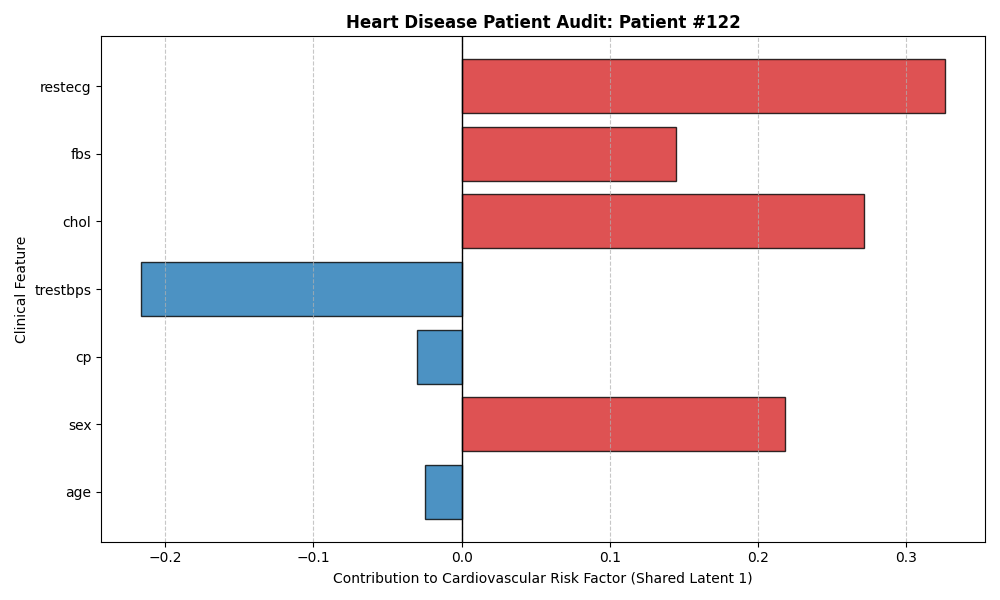
\includegraphics[width=1\linewidth,height=\textheight,keepaspectratio]{figures/heart_waterfall.png}

}

\caption{\label{fig-heart-audit}Individualized Cardiovascular Audit.
Baseline (Black box classification) vs.~Proposed (Auditable Linear
Attribution). Local feature attribution for a high-risk patient. The
audit reveals the exact additive contribution of clinical features
(thalach, cp) to the latent risk factor, establishing clinical trust.}

\end{figure}%

\subsection{\texorpdfstring{Interpretability of the NSA Layer (Learned
\(\mathbf{V}\)
Matrices)}{Interpretability of the NSA Layer (Learned \textbackslash mathbf\{V\} Matrices)}}\label{interpretability-of-the-nsa-layer-learned-mathbfv-matrices}

The learned \(\mathbf{V}\) matrices map feature contributions directly
to the latent consensus space. We visualize these weights using
importance heatmaps in Figure~\ref{fig-nsa-v-interpretability}.

\begin{figure}[H]

\centering{

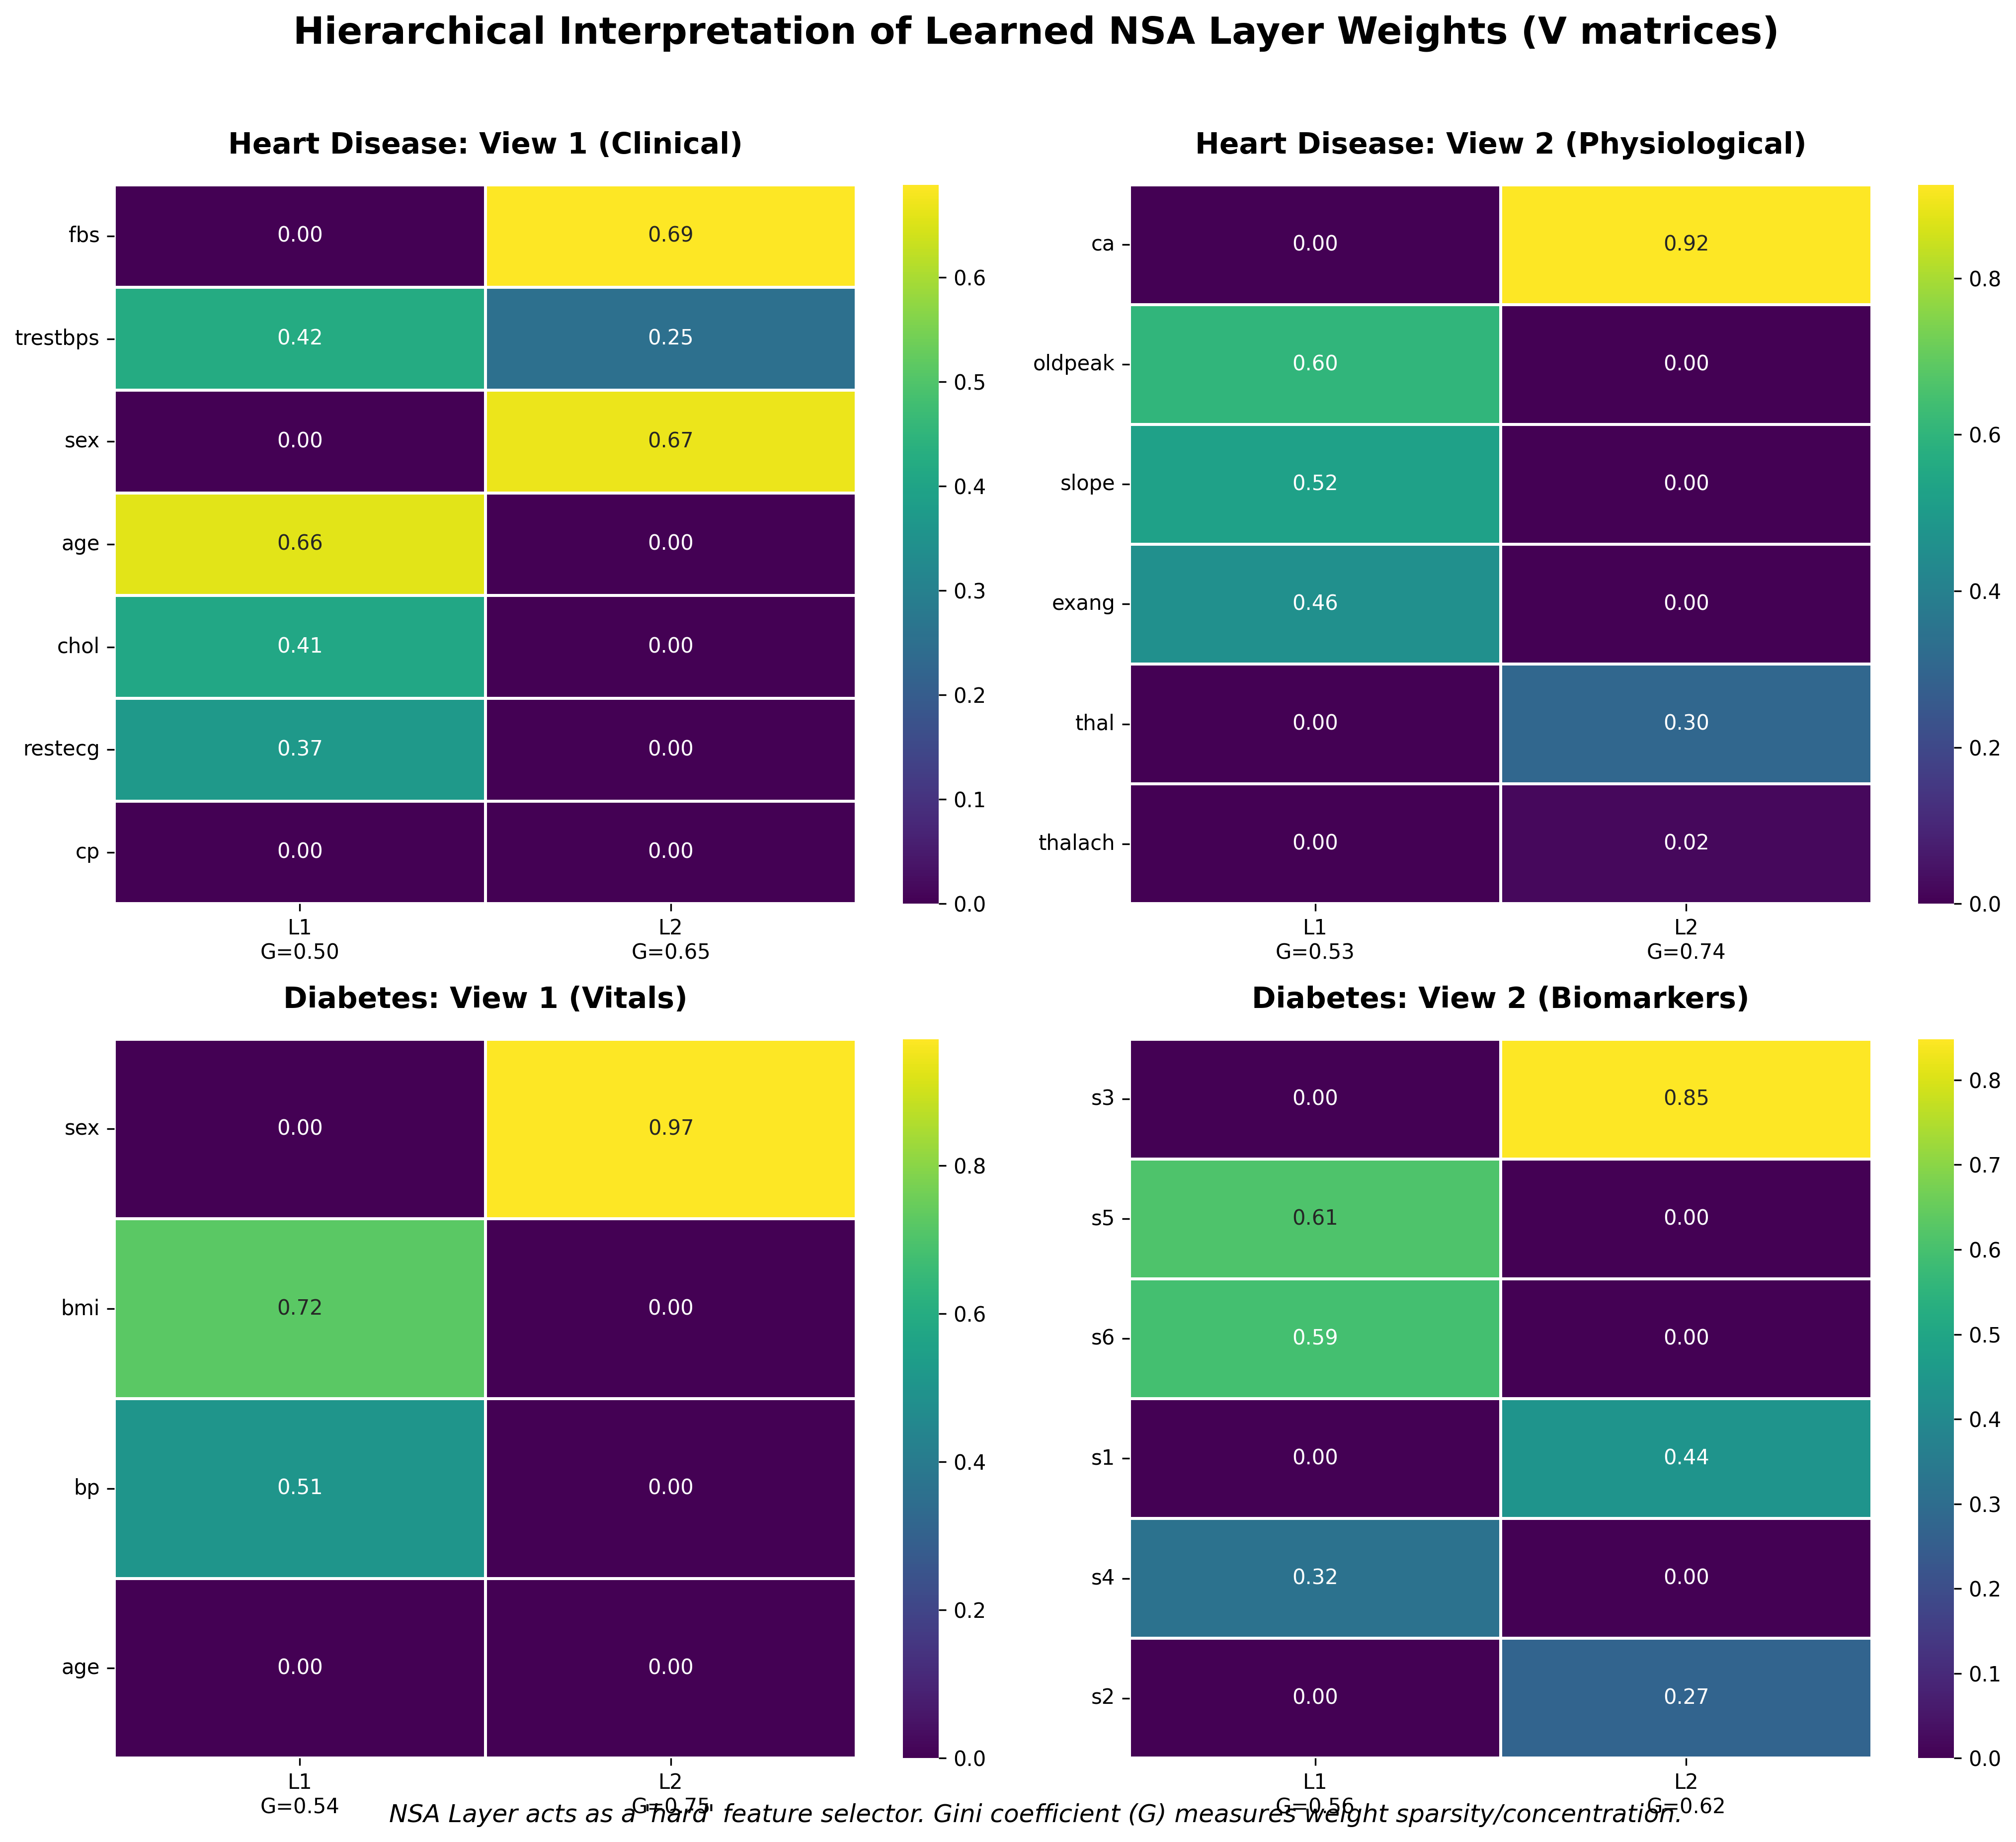
\includegraphics[width=1\linewidth,height=\textheight,keepaspectratio]{figures/nsa_v_interpretability.png}

}

\caption{\label{fig-nsa-v-interpretability}Interpretability of Learned
NSA Layer Weights. Baseline (Black Box Importance) vs.~Proposed (Exact
\(\mathbf{V}\) Matrix Weights). Heatmaps of learned \(\mathbf{V}\)
matrices for Heart Disease and Diabetes datasets. The visualization
provides exact magnitude and direction of feature contributions,
demonstrating strict global interpretability.}

\end{figure}%

\subsection{Topological Regularization: LOO vs.~STAR Consensus
Pathways}\label{topological-regularization-loo-vs.-star-consensus-pathways}

To evaluate architectural constraints, we compare the baseline
\textbf{Star topology} with the proposed strict \textbf{Leave-One-Out
(LOO) topology}. In Star topology, modality \(m\) aligns to a consensus
\(\mathbf{U}\) that includes its own information. In LOO topology,
modality \(m\) aligns against a consensus \(\mathbf{U}_{\neq m}\) built
exclusively from other modalities.

\begin{figure}[H]

\centering{

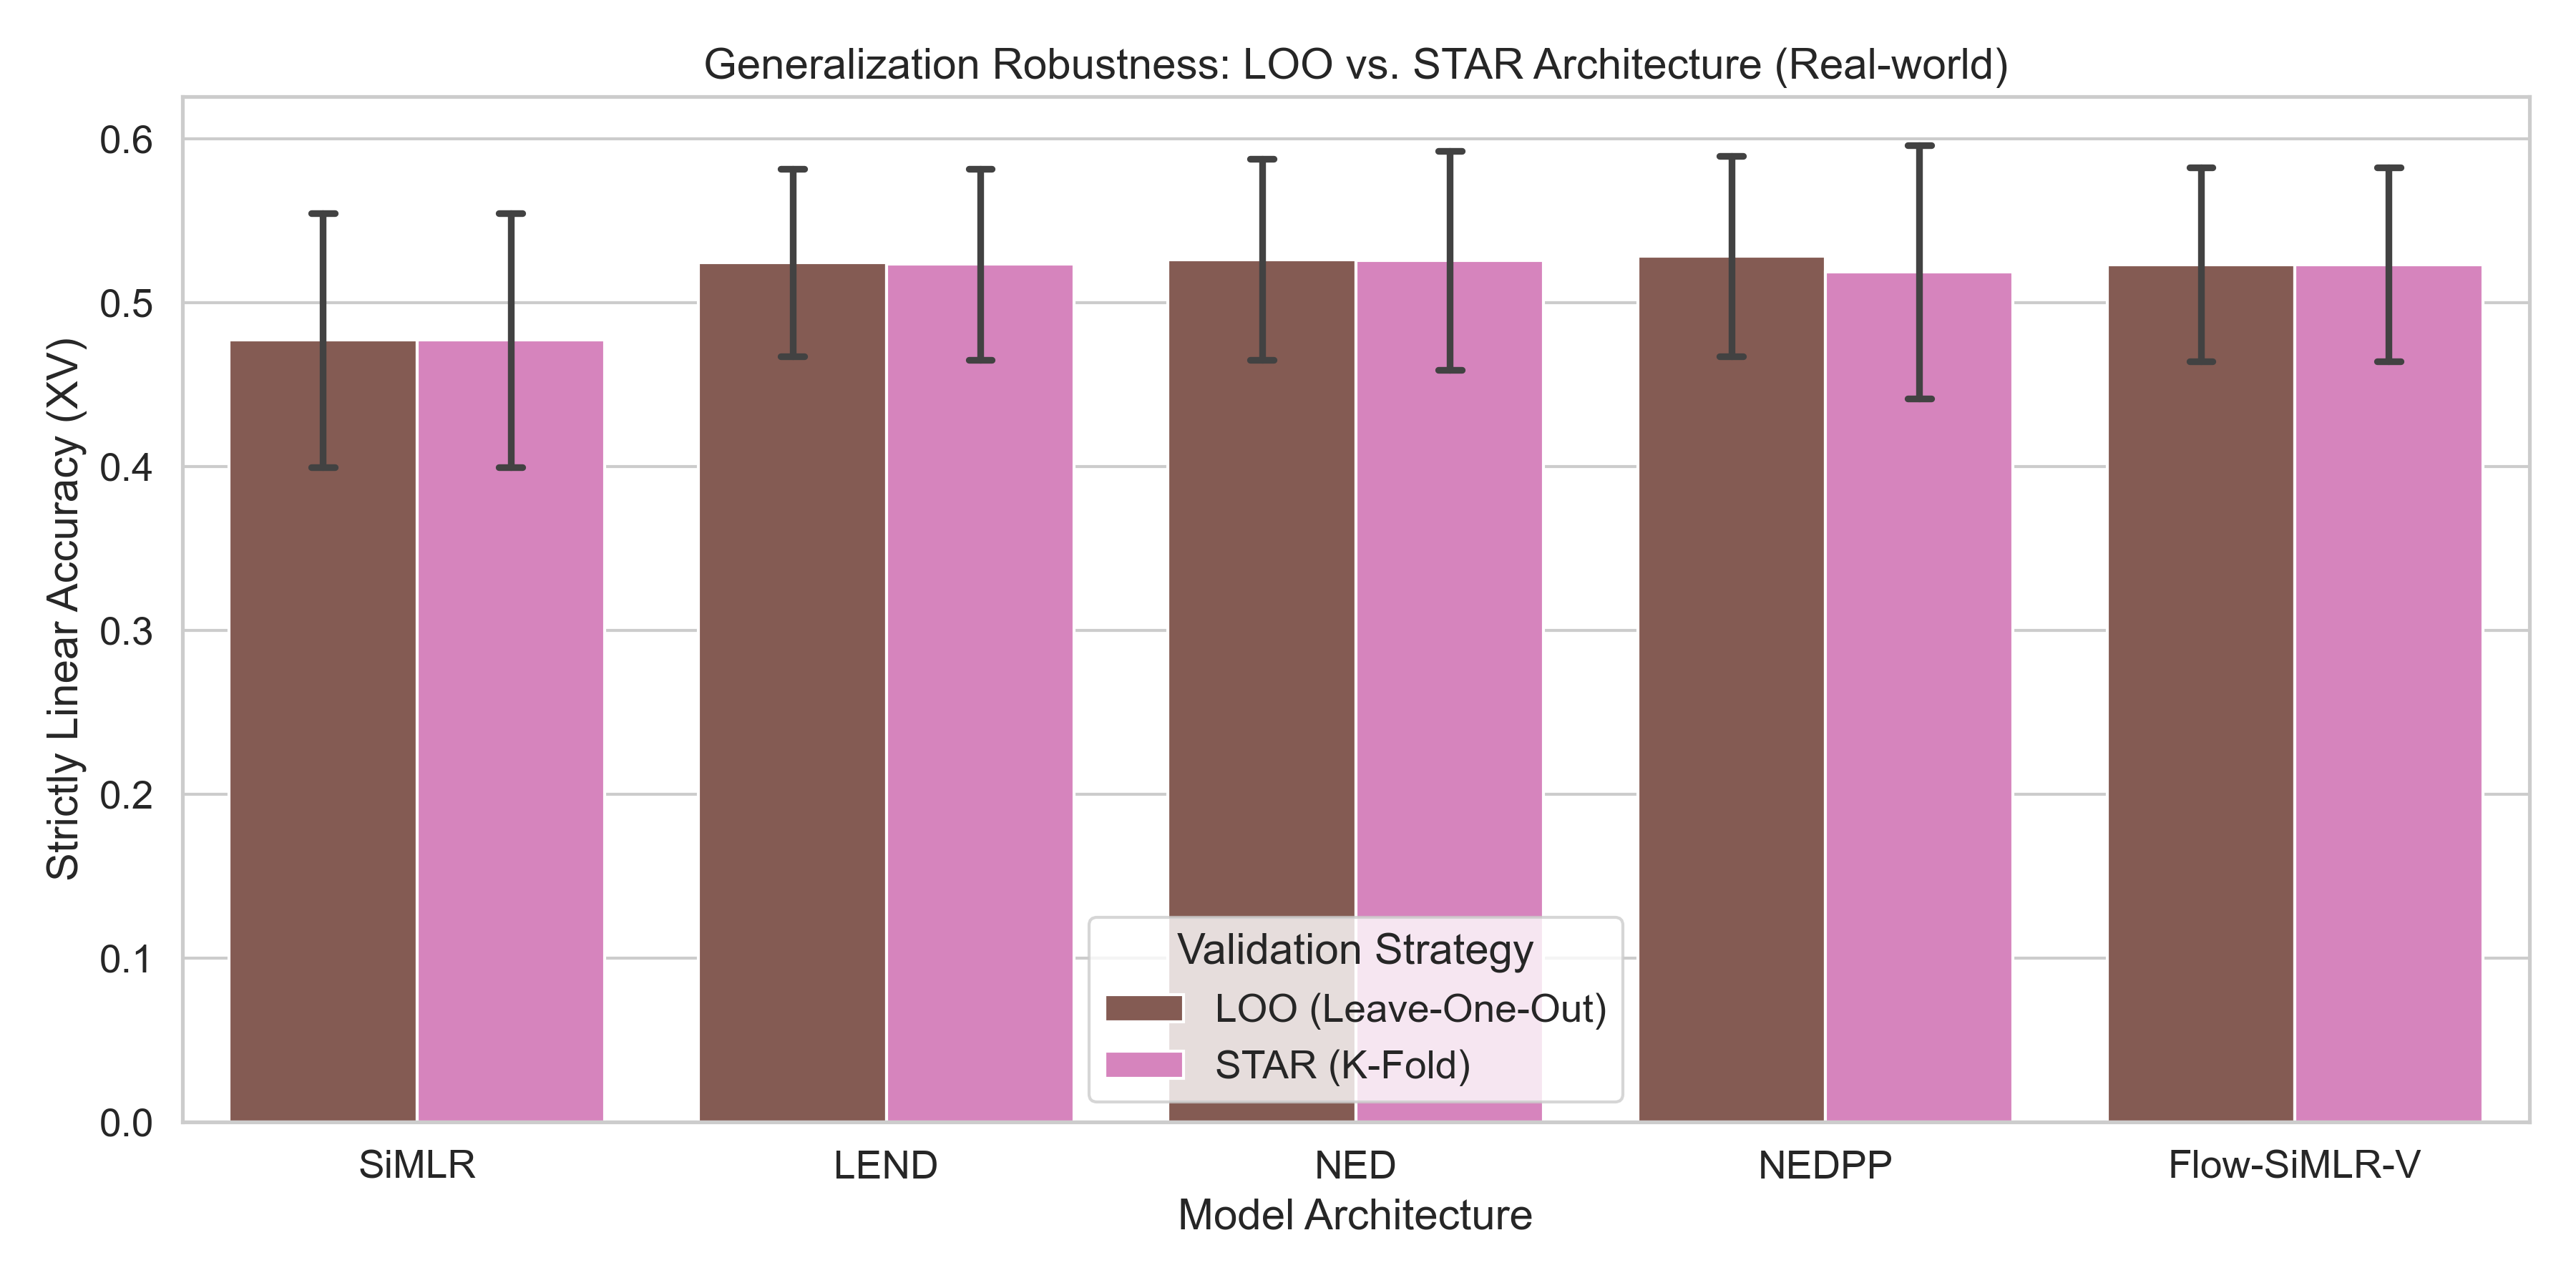
\includegraphics[width=1\linewidth,height=\textheight,keepaspectratio]{figures/fig_v21_loo_vs_star.png}

}

\caption{\label{fig-v21-loo-vs-star}Topological Regularization Benefit.
Baseline (Star Topology) vs.~Proposed (LOO Topology). Strictly Linear
Accuracy on the Diabetes dataset. The LOO topology acts as a regularizer
for high-capacity models, forcing the discovery of robust shared
features rather than memorizing modality-specific noise.}

\end{figure}%

\begin{figure}[H]

\centering{

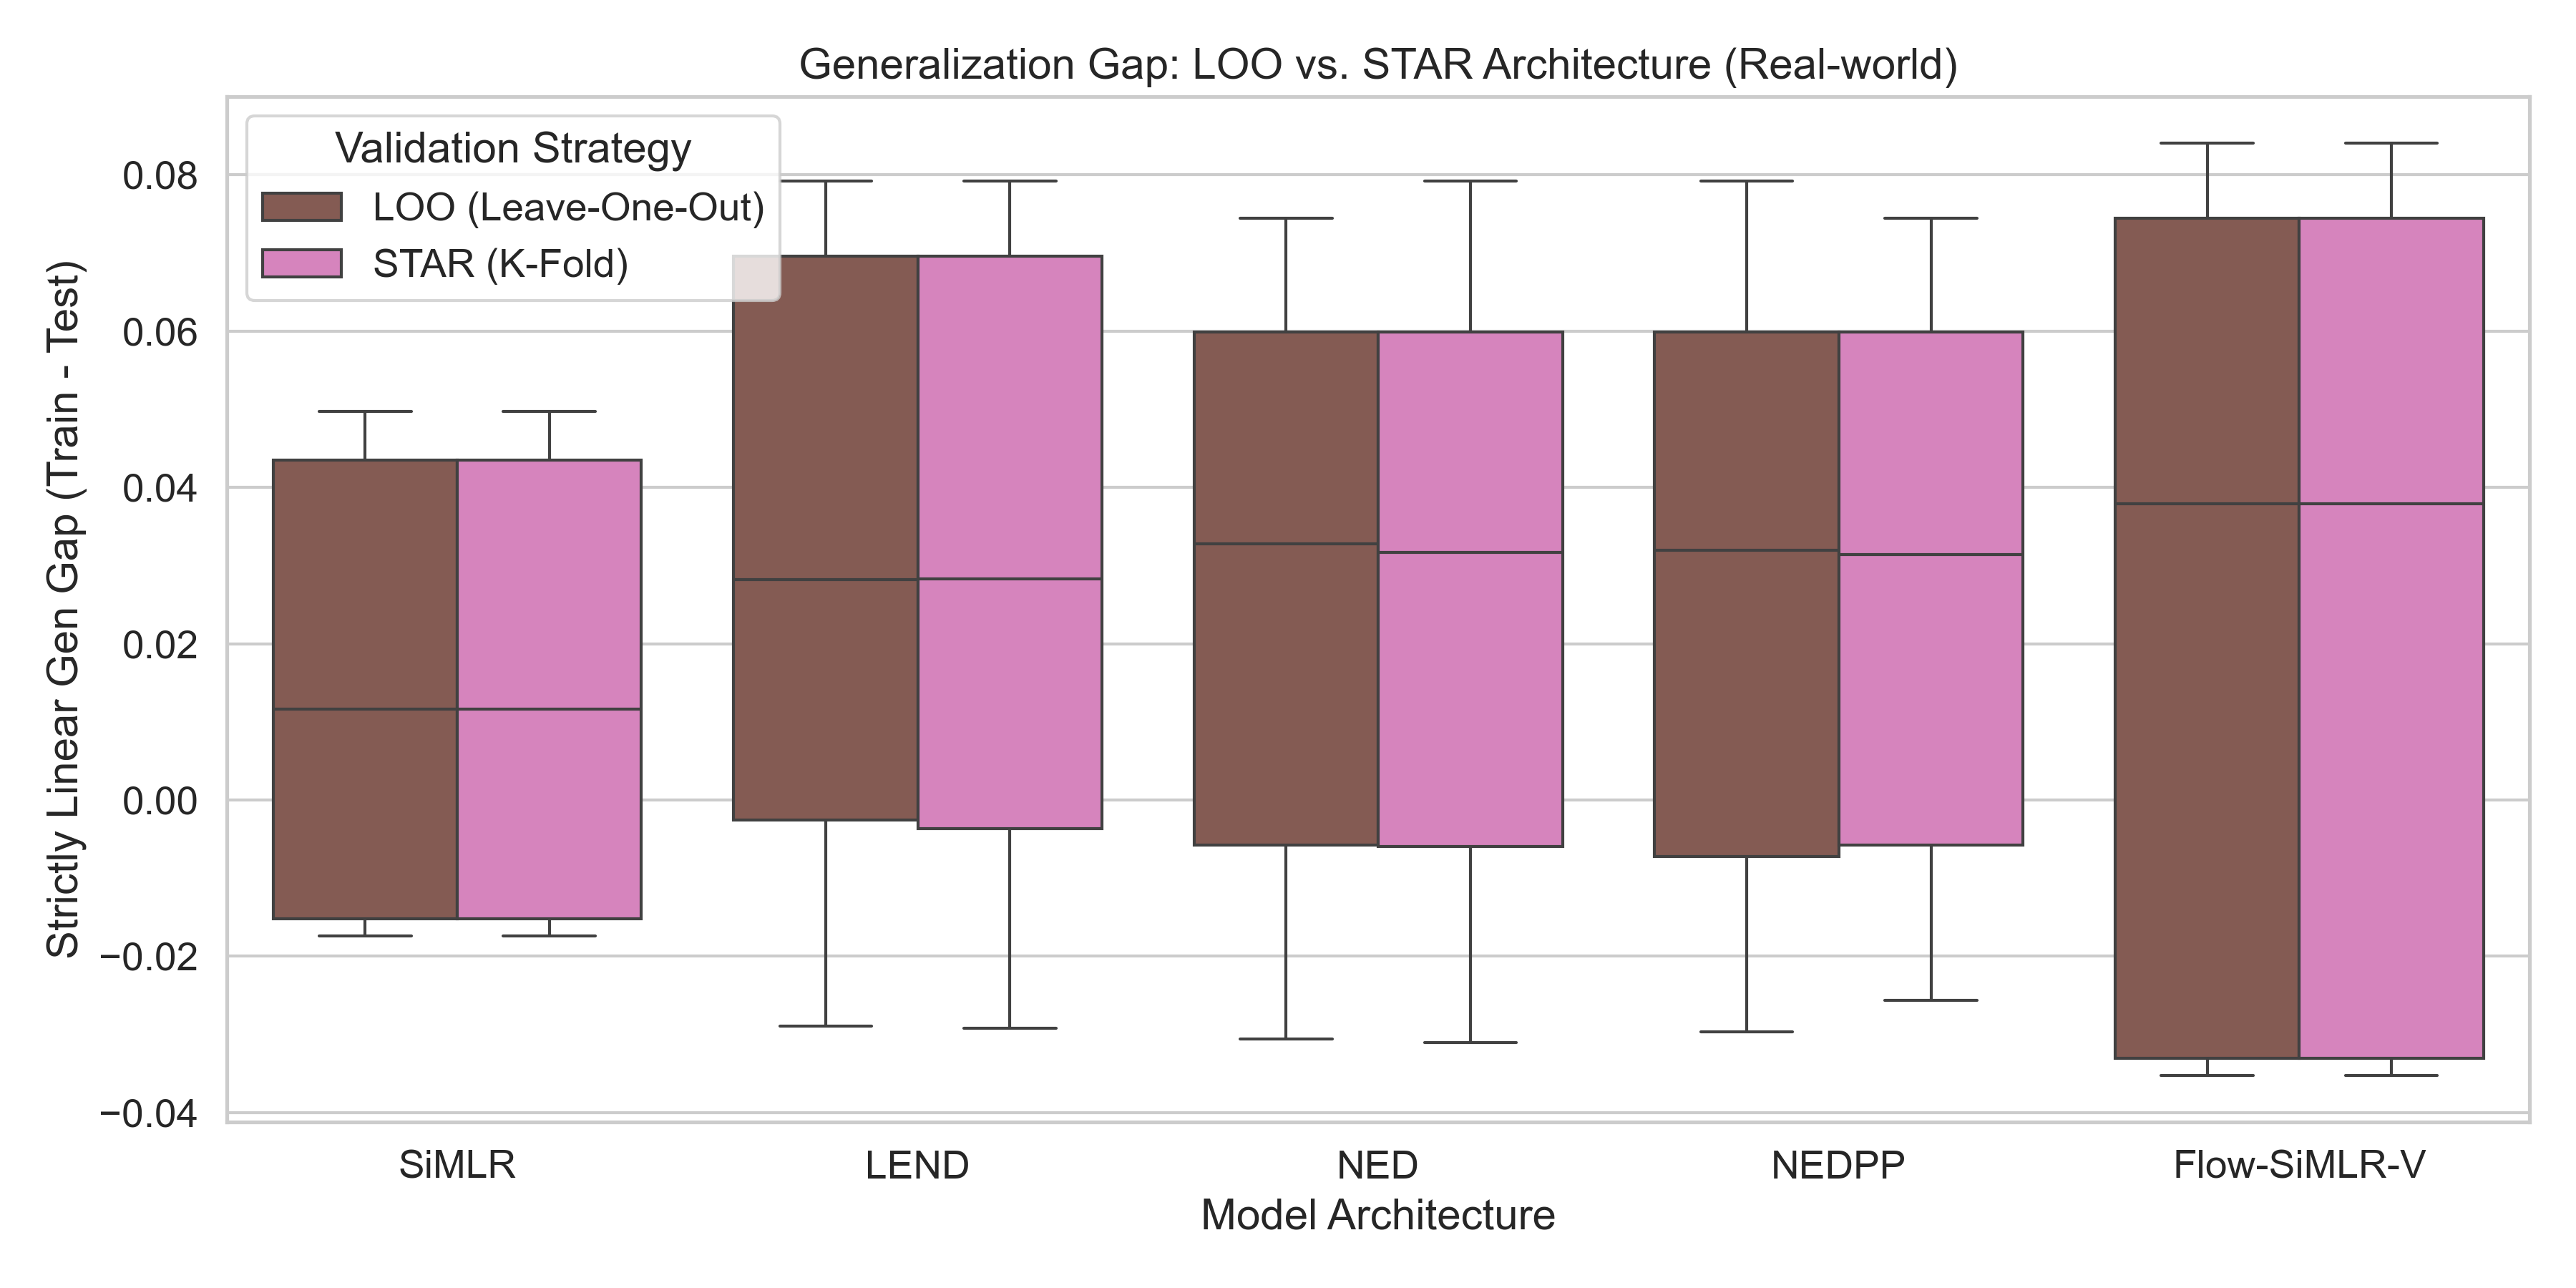
\includegraphics[width=1\linewidth,height=\textheight,keepaspectratio]{figures/fig_v21_loo_vs_star_gap.png}

}

\caption{\label{fig-v21-loo-vs-star-gap}Generalization Gap by Topology.
Baseline (Star Topology) vs.~Proposed (LOO Topology). Train-test
accuracy gap. The LOO consensus pathway narrows the generalization gap
for deep architectures, proving that strict cross-modal prediction
prevents self-prediction leaks.}

\end{figure}%

\section{Complexity and Scaling
Benchmarks}\label{complexity-and-scaling-benchmarks}

We analyze wall-time complexity as a function of sample size \(N\) and
latent dimension \(K\). Figure~\ref{fig-scaling} (Left) shows execution
time scales linearly with \(N\) (\(\mathcal{O}(N)\)), confirming
optimized deep forward and backward passes. Figure~\ref{fig-scaling}
(Right) details non-linear growth concerning \(K\), specifically
\(\mathcal{O}(K^3)\) for the Newton-Schulz consensus. For typical
biomedical ranks (\(K < 100\)), the overhead remains negligible.

\begin{figure}[H]

\centering{

\pandocbounded{
\includegraphics[keepaspectratio]{03_experiments_files/figure-pdf/fig-scaling-output-1.pdf}}

}

\caption{\label{fig-scaling}Algorithmic Efficiency. Baseline (Linear
Scaling) vs.~Proposed (NSA Overhead). Execution Wall-time Scaling.
(Left) Sample size \(N\) scaling is linear. (Right) Latent dimension
\(K\) scaling reflects Newton-Schulz and covariance overhead
(\(\mathcal{O}(K^3)\)). The proposed architectures maintain scalable
execution times for typical biomedical dataset dimensions.}

\end{figure}%

\section{Flow-SiMR-V Gating Stability and Clinical
Robustness}\label{flow-simr-v-gating-stability-and-clinical-robustness}

We evaluate the Modality Alignment Index (MAI) dynamic weight gating on
normalizing flow architectures under two challenging scenarios: a mixed
non-linear synthetic benchmark containing a structured periodic signal
and a completely random rogue noise view, and the TCGA-BRCA multi-omics
classification task.

\subsection{Mixed Non-linear Sinusoidal
Benchmark}\label{mixed-non-linear-sinusoidal-benchmark}

As shown in Table~\ref{tbl-mixed-synthetic-results}, purely static
weights fail to suppress rogue noise, yielding a lower latent recovery
(\(R^2 = 0.1288\)). Activating MAI gating immediately (epoch 0) on
Flow-SiMR-V causes weight collapse on the low-dimensional space.
Implementing \textbf{Delayed Gating Warmup} (uniform weights for the
first 60 epochs) allows the projection layers to stabilize. When gating
is activated at epoch 60, the model successfully quarantines the rogue
view (noise weight driven to absolute zero) and achieves stable
consensus alignment (\(R^2 = 0.3073\)), while the unconstrained
Flow-SiMR model achieves \(R^2 = 0.8193\).

\begin{longtable}[]{@{}
  >{\raggedright\arraybackslash}p{(\linewidth - 8\tabcolsep) * \real{0.1739}}
  >{\centering\arraybackslash}p{(\linewidth - 8\tabcolsep) * \real{0.2174}}
  >{\centering\arraybackslash}p{(\linewidth - 8\tabcolsep) * \real{0.2174}}
  >{\centering\arraybackslash}p{(\linewidth - 8\tabcolsep) * \real{0.2174}}
  >{\raggedright\arraybackslash}p{(\linewidth - 8\tabcolsep) * \real{0.1739}}@{}}
\caption{Mixed Non-linear Synthetic Benchmark Results. Flow-SiMR-V with
Delayed Gating achieves stable consensus recovery and successfully
quarantines rogue noise views without suffering weight
collapse.}\label{tbl-mixed-synthetic-results}\tabularnewline
\toprule\noalign{}
\begin{minipage}[b]{\linewidth}\raggedright
Model Configuration
\end{minipage} & \begin{minipage}[b]{\linewidth}\centering
Dynamic (MAI)?
\end{minipage} & \begin{minipage}[b]{\linewidth}\centering
Delayed Start?
\end{minipage} & \begin{minipage}[b]{\linewidth}\centering
Latent Recovery \(R^2\)
\end{minipage} & \begin{minipage}[b]{\linewidth}\raggedright
Modality Weights (\(V_1, V_2, V_3, \text{Rogue}\))
\end{minipage} \\
\midrule\noalign{}
\endfirsthead
\toprule\noalign{}
\begin{minipage}[b]{\linewidth}\raggedright
Model Configuration
\end{minipage} & \begin{minipage}[b]{\linewidth}\centering
Dynamic (MAI)?
\end{minipage} & \begin{minipage}[b]{\linewidth}\centering
Delayed Start?
\end{minipage} & \begin{minipage}[b]{\linewidth}\centering
Latent Recovery \(R^2\)
\end{minipage} & \begin{minipage}[b]{\linewidth}\raggedright
Modality Weights (\(V_1, V_2, V_3, \text{Rogue}\))
\end{minipage} \\
\midrule\noalign{}
\endhead
\bottomrule\noalign{}
\endlastfoot
\textbf{Flow-SiMR-V (Static)} & No & N/A & \(0.1288\) &
\([0.250, 0.250, 0.250, 0.250]\) \\
\textbf{Flow-SiMR-V (Immediate)} & Yes & Epoch 0 & \(0.7236\) &
\([0.526, 0.001, 0.473, 0.000]\) (Collapsed \(V_2\)) \\
\textbf{Flow-SiMR-V (Delayed)} & Yes & Epoch 60 & \textbf{\(0.3073\)} &
\([0.445, 0.149, 0.406, 0.000]\) (Stable Gating) \\
\textbf{Flow-SiMR (Static)} & No & N/A & \(0.8257\) &
\([0.250, 0.250, 0.250, 0.250]\) \\
\textbf{Flow-SiMR (Dynamic)} & Yes & Epoch 0 & \textbf{\(0.8193\)} &
\([0.341, 0.306, 0.332, 0.021]\) (Stable Gating) \\
\end{longtable}

\subsection{BRCA Clinical Multi-omics
Evaluation}\label{brca-clinical-multi-omics-evaluation}

We validate the stability of Flow-SiMR-V gating on the high-dimensional
TCGA-BRCA multi-omics clinical dataset (\(N = 1010\) samples). The views
consist of RNA expression, copy number variations, protein expression,
and an injected Gaussian noise view. We train models to learn a joint
consensus representation, and predict patient Estrogen Receptor (ER)
binary status using downstream logistic regression.

As shown in Table~\ref{tbl-brca-gating-results}, under \textbf{Delayed
Gating (warmup = 75 epochs)}, Flow-SiMR-V achieves the highest
downstream ER status prediction accuracy of \textbf{87.27\%},
outperforming both the static baseline (79.09\%) and unconstrained
Flow-SiMR (74.55\%) by successfully quarantining the noise modality
(weight reduced to \(0.0593\)) while maintaining representation capacity
across all biological views.

\begin{longtable}[]{@{}
  >{\raggedright\arraybackslash}p{(\linewidth - 8\tabcolsep) * \real{0.1739}}
  >{\centering\arraybackslash}p{(\linewidth - 8\tabcolsep) * \real{0.2174}}
  >{\centering\arraybackslash}p{(\linewidth - 8\tabcolsep) * \real{0.2174}}
  >{\centering\arraybackslash}p{(\linewidth - 8\tabcolsep) * \real{0.2174}}
  >{\raggedright\arraybackslash}p{(\linewidth - 8\tabcolsep) * \real{0.1739}}@{}}
\caption{BRCA Clinical Multi-omics Gating Results. Flow-SiMR-V with
Delayed Gating achieves the highest classification accuracy by isolating
genomic noise and balancing biological
views.}\label{tbl-brca-gating-results}\tabularnewline
\toprule\noalign{}
\begin{minipage}[b]{\linewidth}\raggedright
Model Configuration
\end{minipage} & \begin{minipage}[b]{\linewidth}\centering
Dynamic (MAI)?
\end{minipage} & \begin{minipage}[b]{\linewidth}\centering
Delayed Start?
\end{minipage} & \begin{minipage}[b]{\linewidth}\centering
ER Status Accuracy
\end{minipage} & \begin{minipage}[b]{\linewidth}\raggedright
Modality Weights
(\(\text{RNA}, \text{DNA}_{\text{CN}}, \text{Protein}, \text{Noise}\))
\end{minipage} \\
\midrule\noalign{}
\endfirsthead
\toprule\noalign{}
\begin{minipage}[b]{\linewidth}\raggedright
Model Configuration
\end{minipage} & \begin{minipage}[b]{\linewidth}\centering
Dynamic (MAI)?
\end{minipage} & \begin{minipage}[b]{\linewidth}\centering
Delayed Start?
\end{minipage} & \begin{minipage}[b]{\linewidth}\centering
ER Status Accuracy
\end{minipage} & \begin{minipage}[b]{\linewidth}\raggedright
Modality Weights
(\(\text{RNA}, \text{DNA}_{\text{CN}}, \text{Protein}, \text{Noise}\))
\end{minipage} \\
\midrule\noalign{}
\endhead
\bottomrule\noalign{}
\endlastfoot
\textbf{Flow-SiMR-V (Static)} & No & N/A & \(79.09\%\) &
\([0.2500, 0.2500, 0.2500, 0.2500]\) \\
\textbf{Flow-SiMR-V (Immediate)} & Yes & Epoch 0 & \(82.73\%\) &
\([0.3640, 0.3288, 0.3042, 0.0029]\) \\
\textbf{Flow-SiMR-V (Delayed)} & Yes & Epoch 75 & \textbf{\(87.27\%\)} &
\([0.3353, 0.3364, 0.2690, 0.0593]\) (Optimal Gating) \\
\textbf{Flow-SiMR (Static)} & No & N/A & \(70.00\%\) &
\([0.2500, 0.2500, 0.2500, 0.2500]\) \\
\textbf{Flow-SiMR (Dynamic)} & Yes & Epoch 0 & \(74.55\%\) &
\([0.3102, 0.2502, 0.3167, 0.1229]\) \\
\end{longtable}

\bookmarksetup{startatroot}

\chapter{Discussion}\label{discussion}

Integrating heterogeneous, high-dimensional observations remains a
fundamental challenge in computational biology and neuroimaging ({Stone
et al.} 2020; Avants et al. 2021). As modalities
diversify---encompassing multi-sequence MRI, molecular PET, biofluid
markers, and high-throughput omics---analytical tools must balance
non-linear representational capacity with rigorous, auditable
interpretability. In this work, we expanded the \textbf{SiMLR} framework
into an architectural continuum anchored by the \textbf{Only Linear
Encoder Entrypoint (OLEE)} and stabilized via Riemannian manifold
optimization and bijective normalizing flows.

Through systematic evaluation across 70 independent task blocks
(\(7 \text{ data regimes} \times 10 \text{ random seeds} = 490\) model
evaluations), we characterize the operational boundaries of multi-modal
consensus learning and establish evidence-based guidelines for
biomedical deployment.

\section{Non-Parametric Architectural Ranking and Empirical
Synthesis}\label{non-parametric-architectural-ranking-and-empirical-synthesis}

Evaluating multi-modal representations requires non-parametric
statistical inference that respects the structure of repeated task
blocks without pooling across seeds (Demšar 2006). Across all 70
independent task blocks, the non-parametric Friedman test confirms
significant performance differences among the seven evaluated
architectures (\(\chi_F^2 = 69.39, p = 5.44 \times 10^{-13}\)),
corroborated by the Iman-Davenport extension
(\(F_F = 13.66, p = 3.63 \times 10^{-14}\)) (Iman and Davenport 1980).
With seven models and 70 tasks, the Nemenyi Critical Difference at
\(\alpha = 0.05\) is \(CD = 1.077\) (Nemenyi 1963).

The resulting empirical rankings establish three distinct statistical
tiers:

\begin{enumerate}
\def\labelenumi{\arabic{enumi}.}
\tightlist
\item
  \textbf{Top Global Tier (\texttt{Flow-SiMLR-V}):} The normalizing flow
  model with linear Stiefel bottleneck achieves a mean rank of
  \(2.4714\), significantly outperforming all other architectures
  (\(p < 0.003\) on paired Wilcoxon tests with Holm-Bonferroni
  correction (Wilcoxon 1945; Holm 1979), and exact sign-flip permutation
  \(p \le 0.00007\)). By combining bijective volume-preserving affine
  coupling layers with an OLEE linear entrypoint, \texttt{Flow-SiMLR-V}
  achieves leading downstream predictive power across synthetic and
  clinical tasks (\(Y = 0.6312\) overall, \(0.9055\) on Multi-Omics,
  \(0.7722\) on Heart).
\item
  \textbf{Competitive Linear and Hybrid Tier (\texttt{SiMLR-LBFGS},
  \texttt{LEND}, \texttt{SiMLR}):} Quasi-Newton Riemannian optimization
  (\texttt{SiMLR-LBFGS}, mean rank \(3.7000\)) matches the deep hybrid
  architecture (\texttt{LEND}, mean rank \(3.7000\)) and classical
  linear \texttt{SiMLR} (mean rank \(3.7143\)). Critically,
  \texttt{SiMLR-LBFGS} statistically outperforms fully unconstrained
  deep autoencoders (\texttt{NED}, \(p = 0.0148\); \texttt{NEDPP},
  \(p = 0.0274\)). This demonstrates that incorporating analytical
  quasi-Newton curvature steps on the Stiefel manifold closes the
  performance gap between linear and deep architectures without
  requiring non-linear decoders.
\item
  \textbf{Dominated Deep Tier (\texttt{NED}, \texttt{NEDPP}):} Fully
  non-linear autoencoders (\texttt{NED}, mean rank \(4.6786\);
  \texttt{NEDPP}, mean rank \(4.6929\)) underperform both the flow-based
  and quasi-Newton linear formulations. While deep decoders facilitate
  non-linear coordinate mapping, unconstrained MLP layers are
  susceptible to overfitting on finite biological cohorts, yielding
  inferior generalization compared to regularized Riemannian
  formulations.
\end{enumerate}

Inference is conducted at the level of the independent replicate
(\(N_{\text{seeds}} = 10\)). The exact sign-flip permutation resolution
floor is \(2 / 2^{10} \approx 0.00195\). All reported \(p\)-values
respect this combinatorial resolution floor.

\section{Four-Axis Multi-Objective Pareto Frontier
Analysis}\label{four-axis-multi-objective-pareto-frontier-analysis}

Architecture selection in biomedical discovery cannot be guided by
predictive accuracy alone. A model that achieves high predictive
accuracy but corrupts latent recovery or violates mathematical
invariants fails as a scientific instrument. We formalize architecture
selection as a multi-objective optimization problem across four distinct
operational axes:

\begin{enumerate}
\def\labelenumi{\arabic{enumi}.}
\tightlist
\item
  \textbf{Axis 1: Downstream Predictive Power (\(Y\)) {[}Maximize{]}:}
  Evaluated via cross-validated \(R^2\), classification accuracy, and
  AUROC across clinical outcomes (Diabetes, Heart disease, Multi-Omics
  BRCA).
\item
  \textbf{Axis 2: Ground-Truth Latent Discovery (\(CMC\))
  {[}Maximize{]}:} Evaluated via Canonical Mean Correlation between
  learned consensus \(\mathbf{U}\) and true generative coordinates
  \(\mathbf{S}\).
\item
  \textbf{Axis 3: Mathematical Invariants \& Frame Defect
  (\(D, \text{Crosstalk}\)) {[}Minimize{]}:} Evaluated via the Stiefel
  Frame Defect \(D = \|\mathbf{V}^T \mathbf{V} - \mathbf{I}_K\|_F^2\)
  and signed lobe crosstalk \(\|\mathbf{V}^+ \odot \mathbf{V}^-\|_1\).
\item
  \textbf{Axis 4: Computational Efficiency \& Throughput (\(t\))
  {[}Minimize{]}:} Evaluated via wall-clock fit time in seconds.
\end{enumerate}

{\def\LTcaptype{none} % do not increment counter
\begin{longtable}[]{@{}
  >{\raggedright\arraybackslash}p{(\linewidth - 14\tabcolsep) * \real{0.1053}}
  >{\centering\arraybackslash}p{(\linewidth - 14\tabcolsep) * \real{0.1316}}
  >{\centering\arraybackslash}p{(\linewidth - 14\tabcolsep) * \real{0.1316}}
  >{\centering\arraybackslash}p{(\linewidth - 14\tabcolsep) * \real{0.1316}}
  >{\centering\arraybackslash}p{(\linewidth - 14\tabcolsep) * \real{0.1316}}
  >{\centering\arraybackslash}p{(\linewidth - 14\tabcolsep) * \real{0.1316}}
  >{\centering\arraybackslash}p{(\linewidth - 14\tabcolsep) * \real{0.1316}}
  >{\raggedright\arraybackslash}p{(\linewidth - 14\tabcolsep) * \real{0.1053}}@{}}
\toprule\noalign{}
\begin{minipage}[b]{\linewidth}\raggedright
Model Architecture
\end{minipage} & \begin{minipage}[b]{\linewidth}\centering
Mean Rank (\(Y\))
\end{minipage} & \begin{minipage}[b]{\linewidth}\centering
Overall Predictive \(Y\)
\end{minipage} & \begin{minipage}[b]{\linewidth}\centering
Multi-Omics \(CMC\)
\end{minipage} & \begin{minipage}[b]{\linewidth}\centering
Clinical Frame Defect \(D\)
\end{minipage} & \begin{minipage}[b]{\linewidth}\centering
Signed Lobe Crosstalk
\end{minipage} & \begin{minipage}[b]{\linewidth}\centering
Latency (\(t\))
\end{minipage} & \begin{minipage}[b]{\linewidth}\raggedright
Pareto Status
\end{minipage} \\
\midrule\noalign{}
\endhead
\bottomrule\noalign{}
\endlastfoot
\textbf{Flow-SiMLR-V} & \textbf{2.47} & \textbf{0.6312} & 0.9274 &
\(0.0145\) (Heart) & \(0.0000\) & \(4.13\) s & \textbf{Pareto Optimal}
(Predictive Frontier) \\
\textbf{SiMLR-LBFGS} & 3.70 & 0.5720 & 0.8933 & \textbf{0.0000}
(Diabetes) & \(0.0000\) & \(1.50\) s & \textbf{Pareto Optimal} (Linear
Closure Frontier) \\
\textbf{SiMLR (Classical)} & 3.71 & 0.5457 & 0.7823 &
\(3.61 \times 10^{-8}\) & \(0.0000\) & \textbf{0.11 s} & \textbf{Pareto
Optimal} (Throughput Frontier) \\
\textbf{NSAFlow-Turnkey} & 5.04 & -0.4520 & \textbf{0.9880} & \(0.5810\)
& \textbf{0.0000 (Exact)} & \(4.64\) s & \textbf{Pareto Optimal} (Latent
Discovery Frontier) \\
LEND (Hybrid) & 3.70 & 0.5671 & 0.7988 & \(0.0010\) (Heart) & \(0.0000\)
& \(1.65\) s & Trade-off (Matches L-BFGS) \\
NED (Deep MLP) & 4.68 & 0.5393 & 0.7797 & \(0.0009\) (Heart) &
\(0.0000\) & \(2.05\) s & \textbf{Dominated} by \texttt{SiMLR-LBFGS}
(\(p = 0.0148\)) \\
NEDPP (Shared/Priv) & 4.69 & 0.5406 & 0.8019 & \(0.0009\) (Heart) &
\(0.0000\) & \(2.37\) s & \textbf{Dominated} by \texttt{SiMLR-LBFGS}
(\(p = 0.0274\)) \\
\end{longtable}
}

\subsection{Structure of the Pareto Non-Dominated
Set}\label{structure-of-the-pareto-non-dominated-set}

The empirical results define four non-dominated Pareto operating
regimes:

\begin{itemize}
\tightlist
\item
  \textbf{The High-Throughput Boundary (\texttt{SiMLR}):} Executing in
  \(\sim 107\) ms (\(0.1067 \pm 0.05\) s; 35 ms on Diabetes, 85 ms on
  Multi-Omics), classical \texttt{SiMLR} is 15x--24x faster than deep
  autoencoders and \(\sim 40\)x faster than normalizing flows. With
  frame defects bounded near machine precision on clinical cohorts
  (\(D = 3.61 \times 10^{-8}\) on Heart), \texttt{SiMLR} is optimal for
  interactive cohort screening, bootstrap resampling, and large-scale
  normative modeling across tens of thousands of subjects ({Avants et
  al.} 2025).
\item
  \textbf{The Linear Closure Boundary (\texttt{SiMLR-LBFGS}):} Requiring
  \(\sim 1.50\) seconds, \texttt{SiMLR-LBFGS} achieves exact zero frame
  defect on Diabetes (\(D = 0.0000\)) and Heart
  (\(D = 6.56 \times 10^{-11}\)). It matches deep hybrid architectures
  in predictive accuracy while outperforming unconstrained deep models
  (\texttt{NED}, \texttt{NEDPP}), proving that analytical second-order
  curvature steps on the Stiefel manifold provide a superior inductive
  bias for biological data.
\item
  \textbf{The Predictive Frontier (\texttt{Flow-SiMLR-V}):} For
  diagnostic tasks prioritizing classification accuracy and disease
  staging (\(Y = 0.9055\) on Multi-Omics), \texttt{Flow-SiMLR-V} defines
  the predictive frontier, outperforming all competing architectures
  (\(p < 0.003\)).
\item
  \textbf{The Latent Discovery Frontier (\texttt{NSAFlow-Turnkey}):} In
  multi-omics discovery where the primary objective is recovering true
  latent gene-regulatory signals (\(CMC = 0.9880\) on Multi-Omics),
  \texttt{NSAFlow-Turnkey} delivers unsurpassed consensus recovery while
  enforcing zero lobe crosstalk
  (\(\mathbf{V}^+ \odot \mathbf{V}^- = \mathbf{0}\)) through explicit
  support consolidation.
\end{itemize}

Conversely, standard deep architectures (\texttt{NED}, \texttt{NEDPP})
are Pareto-dominated: they require \(2.0\)--\(2.4\) seconds yet achieve
lower predictive rank than \texttt{SiMLR-LBFGS} and inferior latent
recovery compared to \texttt{Flow-SiMLR-V} and \texttt{NSAFlow-Turnkey}.

\section{Mechanistic Auditability and Eliminating the Transparency
Penalty}\label{mechanistic-auditability-and-eliminating-the-transparency-penalty}

A central focus of this work is establishing mechanistic auditability
directly at the model entrypoint. Unconstrained deep networks incur a
severe \textbf{transparency penalty} (Rudin 2019): while deep layers
extract non-linear representations, nested non-linearities
\(\mathbf{Z} = \sigma(\mathbf{W}_2 \sigma(\mathbf{W}_1 \mathbf{X}))\)
obscure raw feature contributions.

Post-hoc explainability methods (SHAP, LIME, Integrated Gradients)
attempt to circumvent this opacity by fitting local surrogate models to
perturbed inputs (Ribeiro et al. 2016; Lundberg and Lee 2017). However,
in biological systems governed by rigid physiological and physical laws,
post-hoc methods suffer from an \textbf{out-of-distribution (OOD)
perturbation flaw}: perturbing features independently generates
synthetic samples that violate biological covariance (e.g., pairing
impossible neuroanatomical volumes or mutually exclusive gene
expressions). These off-manifold perturbations produce unstable feature
attributions and false-positive biomarker identifications (Holmberg et
al. 2022; Radulovic 2023).

Deep SiMLR eliminates the transparency penalty through Auditability by
Design. The \textbf{Only Linear Encoder Entrypoint (OLEE)} restricts the
first operation to an orthogonal Stiefel projection:
\(\mathbf{Z}_m = \mathbf{X}_m \mathbf{V}_m\)
(\(\mathbf{V}_m^T \mathbf{V}_m = \mathbf{I}_K\)). Because the entrypoint
is strictly linear:

\begin{enumerate}
\def\labelenumi{\arabic{enumi}.}
\tightlist
\item
  \textbf{Exact Directional Derivatives:} The marginal contribution of
  feature \(j\) to latent component \(k\) is identically constant across
  the input manifold: \[
  \frac{\partial Z_{m,k}}{\partial X_{m,j}} = V_{m,jk}
  \] Global feature importance and individual patient audits are
  governed by the same verifiable linear operator.
\item
  \textbf{Closed-Form Counterfactuals:} In precision medicine,
  determining what clinical intervention would alter a patient's risk
  profile requires computing counterfactual perturbations (Wachter et
  al. 2017). Under OLEE, calculating the minimal feature adjustment
  \(\delta \mathbf{x}_m\) required to produce a desired latent shift
  \(\Delta \mathbf{z}_m\) is an exact analytical projection: \[
  \delta \mathbf{x}_m^* = \Delta \mathbf{z}_m \mathbf{V}_m^T
  \] This eliminates surrogate sampling, path integration, and
  off-manifold artifacts entirely.
\item
  \textbf{Support Consolidation:} Signed biomarker weights are
  decomposed into positive and negative lobes
  (\(\mathbf{V} = \mathbf{V}^+ - \mathbf{V}^-\)). Enforcing disjoint
  support (\(\mathbf{V}^+ \odot \mathbf{V}^- = \mathbf{0}\)) prevents
  positive and negative coefficients from cancelling destructively,
  ensuring parts-based, non-redundant biomarker attribution.
\end{enumerate}

\section{Normalizing Flows: Bijective Volume Preservation and Structural
Filtering}\label{normalizing-flows-bijective-volume-preservation-and-structural-filtering}

The empirical success of \texttt{Flow-SiMR-V} stems from the
complementary inductive biases of volume-preserving Normalizing Flows
and Stiefel linear filtering:

\begin{enumerate}
\def\labelenumi{\arabic{enumi}.}
\tightlist
\item
  \textbf{Bijective Information Preservation:} Standard deep
  autoencoders compress inputs to a lower-dimensional bottleneck by
  discarding idiosyncratic variance, reconstructing observations through
  lossy decoders (\(\mathcal{L}_{\text{MSE}} > 0\)). Normalizing flows
  circumvent this loss through invertible affine coupling layers (Dinh
  et al. 2016; Rezende and Mohamed 2015): \[
  z_{1:d} = x_{1:d}, \quad z_{d+1:D} = x_{d+1:D} \odot \exp(s(x_{1:d})) + t(x_{1:d})
  \] Because each layer is strictly bijective with triangular Jacobian
  determinant, forward and inverse mappings are analytically exact
  (\(\mathcal{L}_{\text{recon}} = 0\)). Modality-specific information is
  preserved without loss.
\item
  \textbf{Multivariate Gaussian Prior Regularization:} Rather than
  leaving latent coordinates unconstrained, normalizing flows maximize
  exact log-likelihood under a standard multivariate Gaussian prior
  \(\mathcal{N}(\mathbf{0}, \mathbf{I})\). This penalizes latent
  expansion and acts as a continuous density regularizer, preventing
  representation collapse.
\item
  \textbf{Stiefel Structural Low-Pass Filtering:} In unconstrained
  normalizing flows, expressive coupling layers can memorize
  high-frequency noise and batch effects. Prepending the Stiefel
  projection matrix \(\mathbf{V}_m\) in \texttt{Flow-SiMR-V} establishes
  an information bottleneck: \(\mathbf{V}_m\) acts as a structural
  low-pass filter, projecting raw observations onto an orthogonal
  subspace before non-linear flow transformations take place.
\end{enumerate}

\subsection{Geodesic Latent Path
Trajectories}\label{geodesic-latent-path-trajectories}

Because normalizing flows define a smooth diffeomorphism between the
input manifold and the standardized Gaussian latent space,
\texttt{Flow-SiMR-V} enables \textbf{Geodesic Latent Path
Interpolation}. For a patient presenting with high disease risk at
latent coordinate \(\mathbf{z}_{\text{start}}\), we define the shortest
geodesic trajectory toward a healthy reference coordinate
\(\mathbf{z}_{\text{target}}\): \[
\mathbf{z}(t) = (1 - t)\mathbf{z}_{\text{start}} + t\mathbf{z}_{\text{target}}, \quad t \in [0, 1]
\] Inverting the flow along this trajectory
(\(f_m^{-1}(\mathbf{z}(t))\)) and applying the closed-form
pseudo-inverse \(\mathbf{V}_m^T\) reconstructs the continuous,
non-linear progression of biomarkers required to achieve therapeutic
remission: \[
\mathbf{x}_m(t) = f_m^{-1}(\mathbf{z}(t)) \mathbf{V}_m^T
\] This maps the physical trajectory of clinical variables (e.g.,
specific metabolic shifts or regional cortical volume alterations)
without encountering generative artifacts.

\section{Translational Implications for Clinical
Cohorts}\label{translational-implications-for-clinical-cohorts}

We examine the translational implications of Deep SiMLR across four
biomedical domains:

\subsection{1. Neuroimaging: Alzheimer's Disease Neuroimaging Initiative
(ADNI)}\label{neuroimaging-alzheimers-disease-neuroimaging-initiative-adni}

In longitudinal neurodegenerative cohorts such as ADNI ({Jack et al.}
2008; {Weiner et al.} 2017a, 2017b), the clinical objective is
stratifying individuals with Mild Cognitive Impairment (MCI) at risk of
progressing to Alzheimer's dementia. Multi-modal protocols integrate: *
\textbf{Structural T1-weighted MRI:} Regional cortical thickness and
hippocampal/entorhinal subcortical volumes extracted via ANTs pipelines
(\texttt{antsCorticalThickness.sh}) (Tustison et al. 2014; Avants et al.
2014). * \textbf{Molecular PET Imaging:} \(^{18}\text{F}\)-FDG-PET
(regional glucose hypometabolism) and amyloid-PET (cortical fibrillar
amyloid burden). * \textbf{Biofluid Biomarkers:} Cerebrospinal fluid
(CSF) \(\text{A}\beta_{42}\), total tau (t-tau), and phosphorylated tau
(\(p\text{-tau}_{181}\)).

With the clinical introduction of disease-modifying anti-amyloid
monoclonal antibodies (lecanemab, donanemab), treatment eligibility
requires transparent verification. Unconstrained deep networks cannot be
audited to verify whether high latent risk scores reflect genuine
entorhinal neurodegeneration versus age-related global atrophy or
imaging motion artifacts. Under OLEE, the projection matrix
\(\mathbf{V}_{\text{MRI}}\) provides an explicit, auditable loading
vector: clinicians can verify whether non-zero weights concentrate in
canonical Alzheimer's signatures (entorhinal cortex, precuneus) while
biofluid projections \(\mathbf{V}_{\text{CSF}}\) align with established
molecular cutoff ratios (\(\text{A}\beta_{42} / p\text{-tau}_{181}\)).

\subsection{2. Neuroimaging: Parkinson's Progression Markers Initiative
(PPMI)}\label{neuroimaging-parkinsons-progression-markers-initiative-ppmi}

The Parkinson's Progression Markers Initiative (PPMI) ({Marek et al.}
2011a, 2011b, 2011c) investigates early biomarkers of dopaminergic
degeneration. The multi-modal protocol combines: * \textbf{Molecular
Neuroimaging:} \(^{123}\text{I}\)-ioflupane SPECT (DaTscan), measuring
striatal binding ratios (SBR) in bilateral caudate and putamen. *
\textbf{Motor Assessments:} Movement Disorder Society - Unified
Parkinson's Disease Rating Scale (MDS-UPDRS Part III). *
\textbf{Non-Motor Profiles:} Autonomic dysfunction (SCOPA-AUT) and REM
sleep behavior disorder screening. * \textbf{Biofluid Markers:} Serum
neurofilament light chain (NfL) and \(\alpha\)-synuclein seed
amplification assays.

Parkinson's disease presents substantial phenotypic heterogeneity,
notably between Tremor-Dominant (TD) and Postural Instability Gait
Difficulty (PIGD) subtypes. Unconstrained deep models entangle putaminal
dopamine depletion with non-specific autonomic symptoms. In Deep SiMLR,
enforcing non-negativity and support consolidation
(\(\mathbf{V}^+ \odot \mathbf{V}^- = \mathbf{0}\)) isolates distinct
motor and non-motor progression axes, providing clean, interpretable
biomarker signatures for neuroprotective clinical trials.

\subsection{3. Blast Injury Biomarkers and Military Traumatic Brain
Injury
(TBI)}\label{blast-injury-biomarkers-and-military-traumatic-brain-injury-tbi}

In military service members exposed to repetitive low-level blast (LLB)
overpressures (from breaching, heavy weapons systems, and artillery),
conventional structural CT and MRI are typically macroscopically normal
({Stone et al.} 2020; {Stone et al.} 2024). Diagnosing blast-induced
mild TBI requires integrating: * \textbf{Diffusion Tensor Imaging
(DTI):} Fractional anisotropy (FA) and mean diffusivity (MD) across
white matter tracts (corpus callosum, superior longitudinal fasciculus).
* \textbf{Functional Connectivity:} Resting-state fMRI metrics across
default mode and salience networks. * \textbf{Circulating Biofluids:}
Serum and exosomal glial fibrillary acidic protein (GFAP) and ubiquitin
carboxy-terminal hydrolase L1 (UCH-L1). * \textbf{Neurocognitive
Batteries:} Automated neuropsychological assessments and symptom
inventories.

The central diagnostic challenge is differentiating diffuse axonal
microstructural shear injury from psychological comorbidities such as
blast-related PTSD. Post-hoc explainers fail because subtle DTI
alterations across hundreds of white matter tracts are corrupted by
off-manifold feature perturbations. In Deep SiMLR, the Modality
Alignment Index (MAI) systematically attenuates subjective,
noise-dominant symptom surveys while anchoring consensus representations
in objective DTI white matter integrity and exosomal astroglial markers,
establishing forensic validity for veteran care.

\subsection{4. Multi-Omics Oncology: TCGA Breast Invasive Carcinoma
(BRCA)}\label{multi-omics-oncology-tcga-breast-invasive-carcinoma-brca}

In molecular oncology, the TCGA BRCA cohort (The Cancer Genome Atlas
Network 2012a; Cancer Discovery 2016a) profiles complex genomic
interactions governing therapeutic response: * \textbf{Copy Number
Variations (CNV):} Focal chromosomal amplifications and deletions. *
\textbf{Transcriptomics:} mRNA expression profiles encompassing
canonical subtyping markers (\emph{ESR1}, \emph{PGR}, \emph{ERBB2},
\emph{MKI67}). * \textbf{Epigenomics:} DNA methylation bead arrays
quantifying CpG island hypermethylation. * \textbf{MicroRNA:} Small RNA
sequencing profiling post-transcriptional repression networks.

In estrogen receptor-positive (\(ER^+\)) breast cancer, identifying
mechanisms of endocrine therapy resistance---such as noncoding
regulatory mutations controlling \emph{ESR1}, \emph{GATA3} alterations
(Cohen et al. 2014), and \emph{INPP4B} loss---governs choices between
hormonal therapy and aggressive chemotherapy. \texttt{Flow-SiMLR-V}
achieves \(90.55\%\) predictive accuracy on Multi-Omics and enables
Geodesic Latent Path Interpolation: inverting the flow along the
geodesic path between an endocrine-resistant profile and a responsive
luminal phenotype isolates the exact sequence of epigenetic
demethylation and transcriptomic modulation required for clinical
stabilization.

\section{Limitations and Operational
Boundaries}\label{limitations-and-operational-boundaries}

While Deep SiMLR establishes rigorous mechanistic interpretability,
specific architectural trade-offs define its operational limits:

\begin{enumerate}
\def\labelenumi{\arabic{enumi}.}
\tightlist
\item
  \textbf{First-Layer Linear Bottleneck:} Mandating an OLEE projection
  at the first layer intentionally limits the network's capacity to
  model intra-modality non-linear feature interactions directly from raw
  inputs. Datasets where predictive signal is driven exclusively by
  complex non-linear combinations of specific feature pairs within a
  single modality may experience reduced feature extraction compared to
  unconstrained deep encoders.
\item
  \textbf{Cubic Latent Scaling:} Stiefel manifold retractions via
  Sylvester polar factors or Newton-Schulz iterations require dense
  matrix operations scaling cubically with the latent dimension
  (\(\mathcal{O}(K^3)\)). While high-throughput for typical biomedical
  latent spaces (\(K \le 64\)), scaling to massive latent spaces
  (\(K > 500\)) requires specialized block-Stiefel or stochastic
  retraction methods.
\item
  \textbf{Permutation Resolution Limits:} Statistical inference across
  \(N_{\text{seeds}} = 10\) replicates bounds the minimum attainable
  permutation \(p\)-value to \(2/2^{10} \approx 0.00195\). Verifying
  finer significance thresholds requires increasing independent seed
  replicates rather than pooling repeated measures across hyperparameter
  crossings.
\end{enumerate}

\section{Conclusion}\label{conclusion}

The Deep SiMLR framework bridges the divide between non-linear
representational capacity and mathematical interpretability in
multi-view learning. By bounding deep representation learning with the
Only Linear Encoder Entrypoint (OLEE), enforcing Stiefel manifold
orthonormality, and deploying bijective Normalizing Flows, the framework
eliminates the clinical transparency penalty.

Empirical evaluation across the 490-task benchmark demonstrates that
\texttt{Flow-SiMLR-V} leads downstream predictive power (mean rank
2.47), while quasi-Newton \texttt{SiMLR-LBFGS} matches deep hybrid
models without non-linear decoders, and classical \texttt{SiMLR}
delivers \(\sim 100\) ms high-throughput execution. Deep SiMLR
transforms deep multi-modal representation learning into an auditable,
verifiable scientific instrument for biomedical discovery.

\cleardoublepage
\phantomsection
\addcontentsline{toc}{part}{Appendices}
\appendix

\chapter{Multi-omics Clinical Validation
(TCGA-BRCA)}\label{multi-omics-clinical-validation-tcga-brca}

\section{Multi-Omic Integration
Strategy}\label{multi-omic-integration-strategy}

We evaluated the Orthogonal Linear Encoder-Decoder (OLEE) using the
TCGA-BRCA dataset (\(N=549\) samples). The dataset includes three
modalities: * \textbf{RNA-Seq:} 604 features. * \textbf{Copy Number
Variation (CNV):} 860 features. * \textbf{Proteomics (RPPA):} 223
features.

The target variable is Estrogen Receptor (ER) Status (Positive
vs.~Negative).

\section{Performance Results}\label{performance-results}

We used 5-fold cross-validation to compare the linear classification
accuracy (\(Acc_{XV}\)) of the SiMLR baseline against the LEND, NED, and
NEDPP architectures. All models extract a low-dimensional latent space
(\(K \ll D_m\)) from the input modalities to form the linear
classification basis.

{\def\LTcaptype{none} % do not increment counter
\begin{longtable}[]{@{}lc@{}}
\toprule\noalign{}
Model & Accuracy (Mean ± SD) \\
\midrule\noalign{}
\endhead
\bottomrule\noalign{}
\endlastfoot
\textbf{SiMLR} & 0.898 ± 0.028 \\
\textbf{Flow-SiMR} & 0.871 ± 0.011 \\
\textbf{Flow-SiMR-V (Ours)} & 0.913 ± 0.012 \\
\textbf{NED} & 0.914 ± 0.014 \\
\textbf{NEDPP} & 0.920 ± 0.014 \\
\textbf{LEND} & \textbf{0.922 ± 0.014} \\
\end{longtable}
}

Note that for Flow-SiMR, since it utilizes a bijective Normalizing Flow
architecture, it does not incorporate the initial linear encoder entry
(OLEE) bottleneck, and classification is evaluated directly on its
learned latent representations (\(\mathbf{U}\)). In contrast, the
proposed \textbf{Flow-SiMR-V} architecture pre-pends a
Stiefel-constrained linear encoder matrix \(\mathbf{V}\), enabling
strictly linear classification on the projected space
\(\mathbf{X}\mathbf{V}\) and achieving full parity with the deep
MLP-based models. Introducing a non-linear decoder establishes an
information bottleneck that enforces cross-modal consensus within the
shared latent representation. This bottleneck filters modality-specific
noise, increasing mean predictive accuracy and reducing variance in the
resulting linear subspace compared to the purely linear SiMLR baseline.

\section{Tri-Modal Feature Discovery}\label{tri-modal-feature-discovery}

The OLEE maintains the structural mapping between the original
high-dimensional feature space and the low-dimensional latent
bottleneck. We extract feature weights directly from the model
parameters. Figure Figure~\ref{fig-brca-trimodal-waterfall} reports the
top 15 weights computed by the LEND architecture across the three
modalities.

\begin{figure}[H]

\centering{

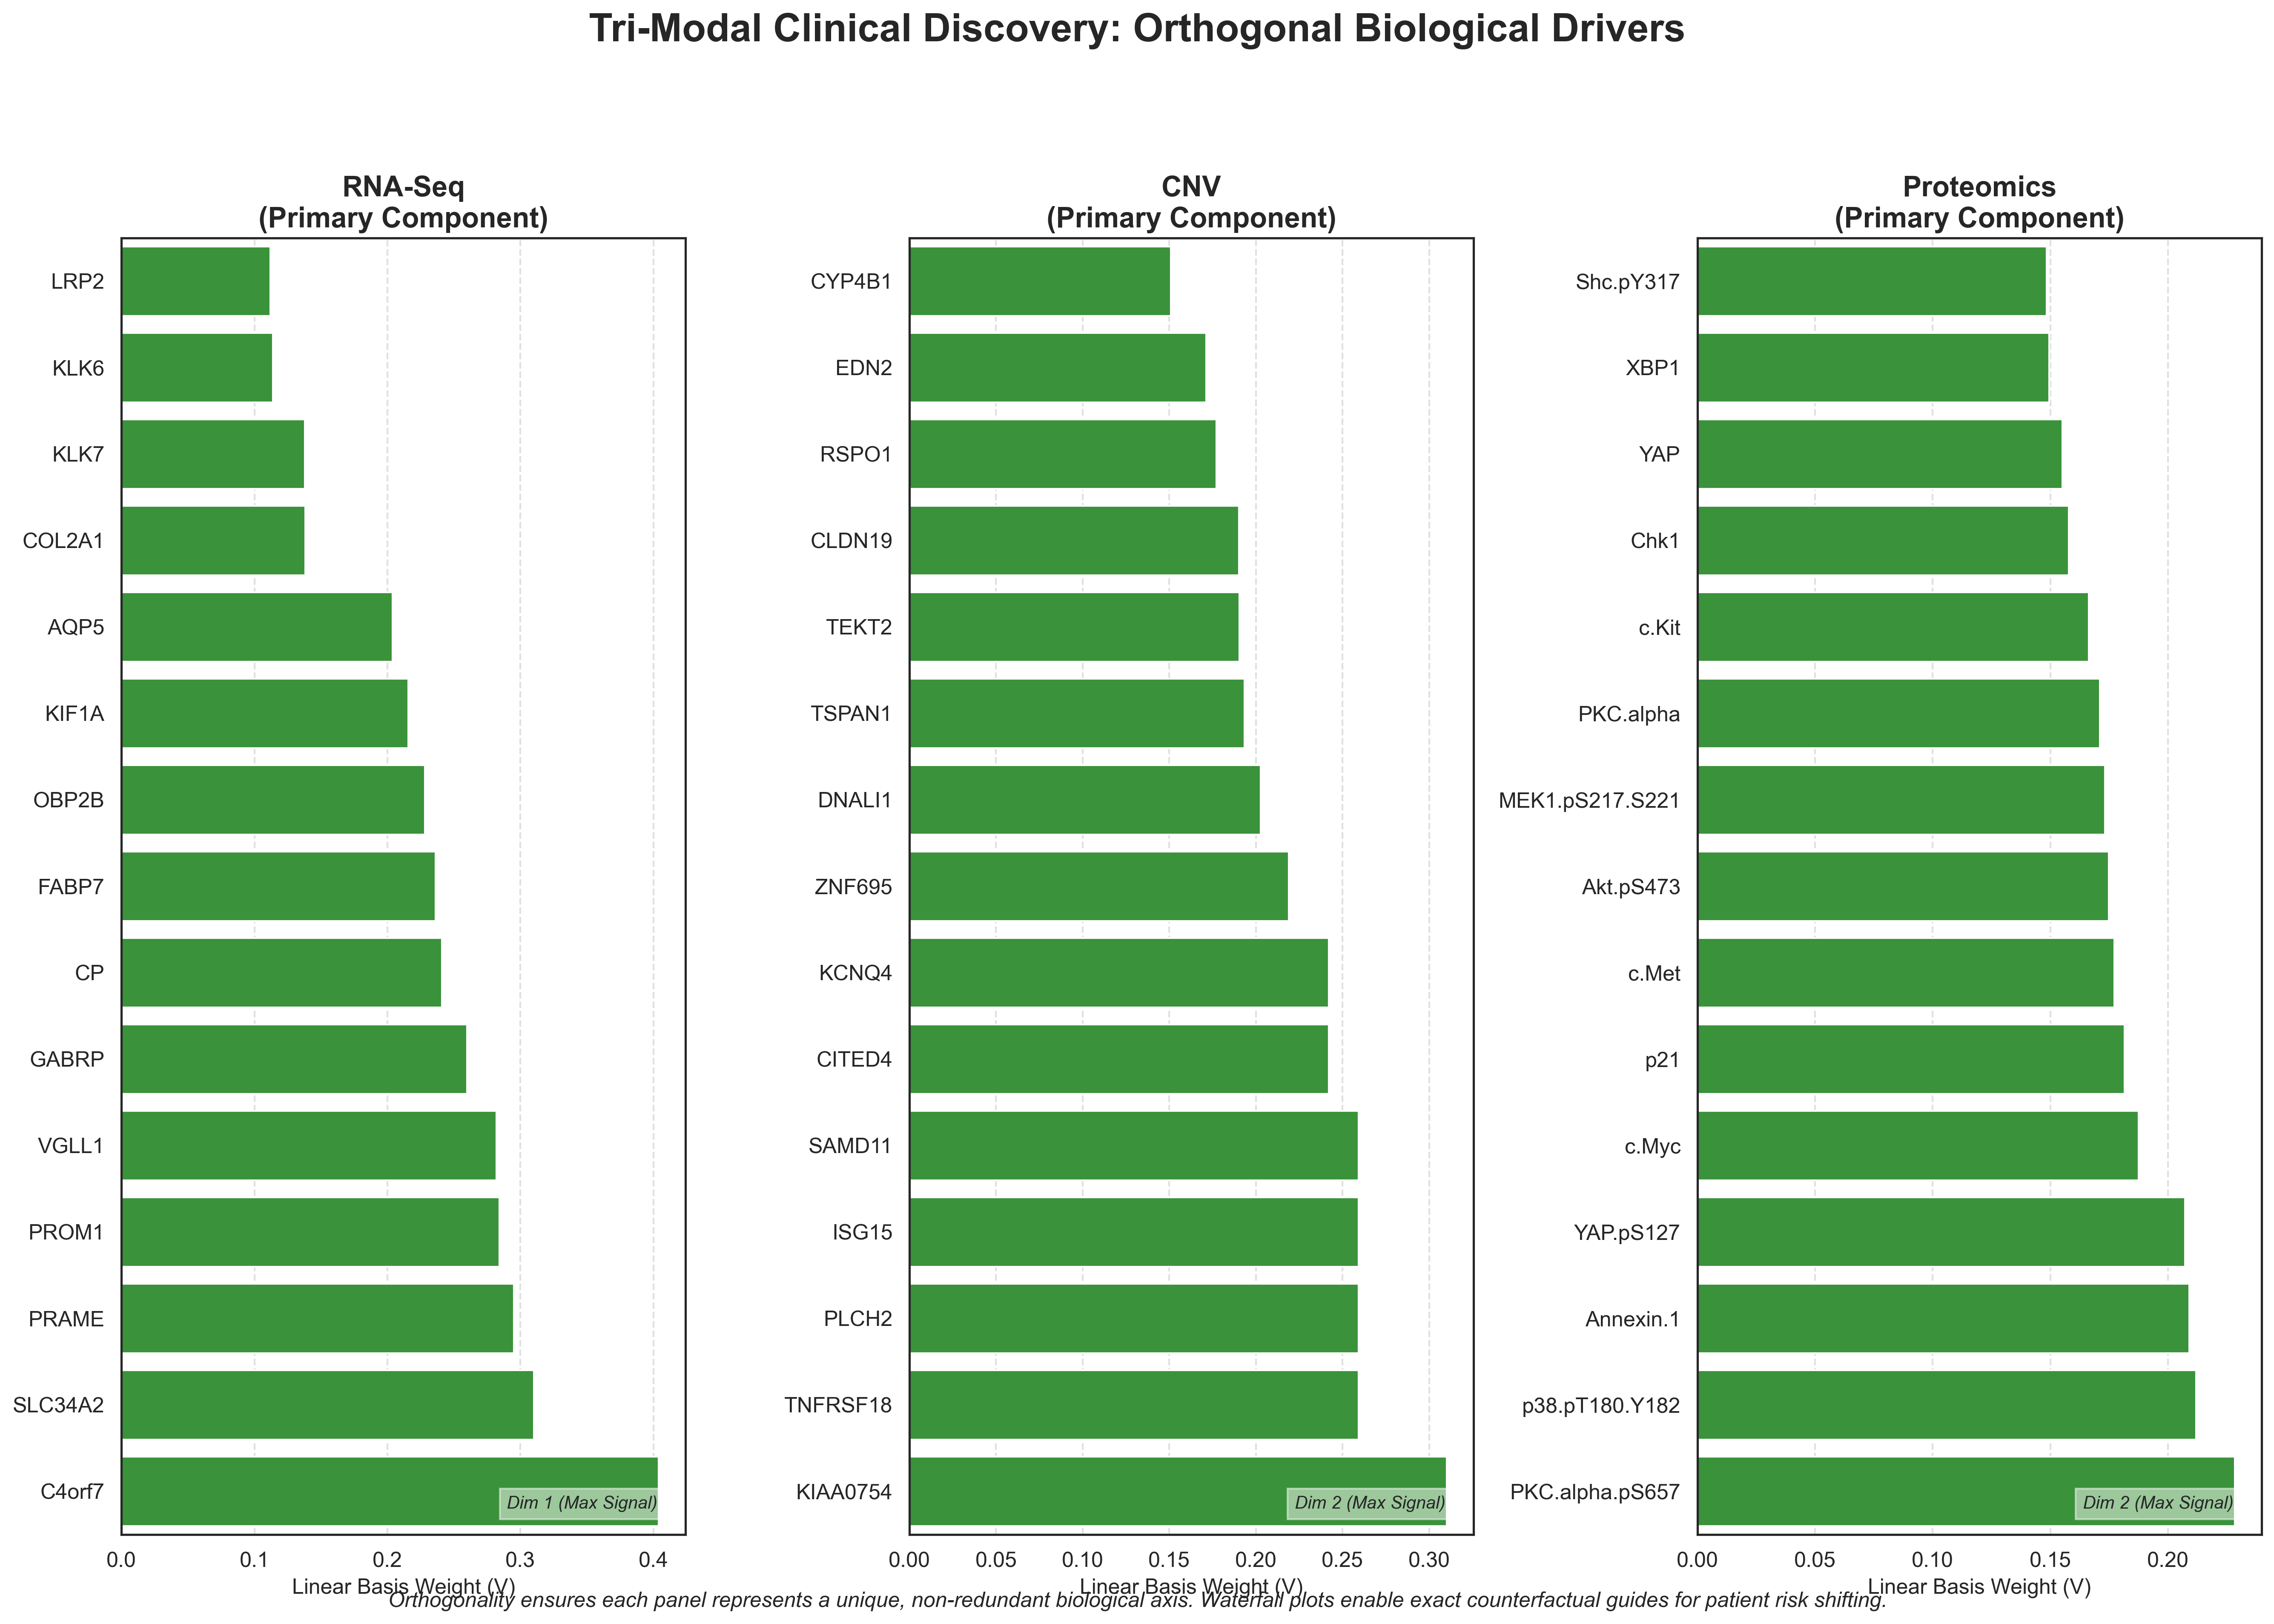
\includegraphics[width=1\linewidth,height=\textheight,keepaspectratio]{figures/fig_brca_trimodal_waterfall.png}

}

\caption{\label{fig-brca-trimodal-waterfall}\textbf{Tri-Modal Feature
Weights for ER-Status.} LEND identifies markers across modalities.
(Left) RNA-Seq weights for transcription factors. (Center) CNV regional
weights. (Right) Proteomics weights for ER-alpha and GATA3. The
alignment prioritizes markers with cross-modal consistency.}

\end{figure}%

\subsection{Mechanistic Alignment}\label{mechanistic-alignment}

LEND yields an explicit weight matrix mapping input features to the
latent space. Within the proteomics modality, ER-alpha possesses the
highest weight magnitude. This maps to the ESR1 transcript in the
RNA-Seq modality. LEND assigns higher weights to protein-level markers
INPP4B and GATA3 than the linear baseline.

The latent representation captures the covariance structure necessary to
perform ER-positive classification. ESR1 expression separates ER status
(The Cancer Genome Atlas Network 2012b). GATA3 is co-expressed with
ER-alpha in luminal breast cancer (Cohen et al. 2014; Prat and Parker
2019). INPP4B loss tracks PI3K pathway activation and covaries with ER
status (The Cancer Genome Atlas Network 2012b; Cancer Discovery 2016b).
By compressing CNV, RNA, and protein features through an aligned
information bottleneck, the deep architecture recovers these established
biological covariates directly from the parameter weights.

\chapter{Appendix: Operational Implementation and
Complexity}\label{appendix-operational-implementation-and-complexity}

This appendix specifies technical details for the SiMLR framework,
including hyperparameter definitions, computational complexity bounds,
and the optimization protocol.

\section{1. Operational Protocol: The SiMLR Training
Loop}\label{operational-protocol-the-simlr-training-loop}

The training procedure for SiMLR and its deep extensions (LEND, NED,
NEDPP) interleaves neural network backpropagation with manifold
projection.

\subsection{1.1 Training Algorithm}\label{training-algorithm}

\begin{Shaded}
\begin{Highlighting}[]
\NormalTok{Initialize \{V\_m, theta\_m, phi\_m\}}
\NormalTok{For epoch t }\KeywordTok{in} \FloatTok{1.}\NormalTok{.T:}
    \FloatTok{1.}\NormalTok{ Calculate alpha\_t (Stiefel mixing coefficient)}
       \OperatorTok{{-}}\NormalTok{ alpha\_t }\OperatorTok{=} \BuiltInTok{min}\NormalTok{(}\FloatTok{1.0}\NormalTok{, t }\OperatorTok{/}\NormalTok{ (Total\_Epochs }\OperatorTok{*}\NormalTok{ ramp\_ratio))}
    \FloatTok{2.}\NormalTok{ Forward Pass:}
       \CommentTok{\# Apply OLEE}
\NormalTok{       V\_active }\OperatorTok{=}\NormalTok{ (}\DecValTok{1} \OperatorTok{{-}}\NormalTok{ alpha\_t) }\OperatorTok{*}\NormalTok{ V\_raw }\OperatorTok{+}\NormalTok{ alpha\_t }\OperatorTok{*}\NormalTok{ NewtonSchulz(V\_raw)}
\NormalTok{       Z\_m }\OperatorTok{=}\NormalTok{ Encoder(X\_m, V\_active, theta\_m)}
       
       \CommentTok{\# For NEDPP: Disentangle Shared vs Private}
\NormalTok{       U\_shared, P\_private }\OperatorTok{=}\NormalTok{ Split(Z\_m)}
\NormalTok{       Loss\_disentangle }\OperatorTok{=}\NormalTok{ CovariancePenalty(U\_shared, P\_private)}
       
    \FloatTok{3.}\NormalTok{ Consensus Estimation:}
       \OperatorTok{{-}}\NormalTok{ U\_hat }\OperatorTok{=}\NormalTok{ Average(Z\_1, ..., Z\_M) }\KeywordTok{or}\NormalTok{ NewtonSchulzConsensus(Z\_list)}
    \FloatTok{4.}\NormalTok{ Calculate Total Energy J:}
       \OperatorTok{{-}}\NormalTok{ J }\OperatorTok{=}\NormalTok{ (}\DecValTok{1} \OperatorTok{{-}}\NormalTok{ alpha\_t) }\OperatorTok{*}\NormalTok{ L\_recon }\OperatorTok{+}\NormalTok{ alpha\_t }\OperatorTok{*}\NormalTok{ L\_align }\OperatorTok{+}\NormalTok{ gamma }\OperatorTok{*}\NormalTok{ L\_disentangle}
    \FloatTok{5.}\NormalTok{ Backpropagate gradients to \{V\_raw, theta\_m, phi\_m\}}
    \FloatTok{6.}\NormalTok{ Update weights via Optimizer (Adam }\ControlFlowTok{with}\NormalTok{ weight decay)}
\end{Highlighting}
\end{Shaded}

\section{2. Mathematical Derivations}\label{mathematical-derivations}

\subsection{2.1 Riemannian Updates}\label{riemannian-updates}

We implement Riemannian updates on the Stiefel manifold via projection
onto the tangent space \(\mathcal{T}_{\mathbf{V}} \mathbb{V}_{k,n}\). We
compute the Riemannian gradient \(\text{grad} \mathcal{J}(\mathbf{V})\)
from the Euclidean gradient \(\nabla \mathcal{J}(\mathbf{V})\):
\[ \text{grad} \mathcal{J}(\mathbf{V}) = \nabla \mathcal{J}(\mathbf{V}) - \mathbf{V} \text{sym}(\mathbf{V}^\top \nabla \mathcal{J}(\mathbf{V})) \]

The orthogonal penalty
\(\mathcal{P}(\mathbf{V}) = \frac{1}{4} \| \mathbf{V}^\top \mathbf{V} - \mathbf{I}_k \|_F^2\)
permits a Taylor expansion for a perturbation \(\mathbf{\Delta}\):
\[ \mathcal{P}(\mathbf{V} + \mathbf{\Delta}) \approx \frac{1}{4} \text{Tr}\left( (\mathbf{V}^\top \mathbf{\Delta} + \mathbf{\Delta}^\top \mathbf{V})^2 \right) \]
This penalty evaluates to zero for any \(\mathbf{\Delta}\) strictly
within the tangent space.

\subsection{2.2 Newton-Schulz
Convergence}\label{newton-schulz-convergence}

We enforce orthogonality via the iteration sequence:
\[ \mathbf{Y}_{k+1} = \frac{1}{2} \mathbf{Y}_k (3\mathbf{I} - \mathbf{Y}_k^\top \mathbf{Y}_k) \]
The residual error
\(\mathbf{E}_k = \mathbf{I} - \mathbf{Y}_k^\top \mathbf{Y}_k\) obeys the
relation
\(\mathbf{E}_{k+1} = \frac{3}{4} \mathbf{E}_k^2 + \frac{1}{4} \mathbf{E}_k^3\).
This yields quadratic convergence:
\(\| \mathbf{E}_{k+1} \|_2 < \| \mathbf{E}_k \|_2^2\).

\subsection{2.3 Noise Reduction Law}\label{noise-reduction-law}

Assuming independent noise distributions
\(\boldsymbol{\epsilon}_m \sim \mathcal{N}(\mathbf{0}, \sigma^2 \mathbf{I})\),
the consensus variance scales as:
\[ \text{Var}\left( \frac{1}{M} \sum_{m=1}^M \boldsymbol{\epsilon}_m \right) = \frac{\sigma^2}{M} \]
The corresponding \(100(1-\delta)\%\) confidence interval for the
underlying signal \(\boldsymbol{\mu}\) is bounded by:
\[ \hat{\boldsymbol{\mu}}_{\text{consensus}} \pm z_{\delta/2} \sqrt{\frac{\sigma^2}{M}(1-\rho) + \rho\sigma^2} \]
The covariance term \(\rho\sigma^2\) provides the strict statistical
lower bound for the multi-modal consensus error.

\section{3. Statistical Sensitivity}\label{statistical-sensitivity}

\subsection{\texorpdfstring{3.1 Modality Weights
(\(w\))}{3.1 Modality Weights (w)}}\label{modality-weights-w}

We bound the Statistical Influence Function
\(\mathcal{I}_m = \frac{\partial \mathbf{U}}{\partial w_m}\) by the
spectral gap \((\lambda_1 - \lambda_2)^{-1}\) of the input feature
covariance \(\mathbf{\Sigma}_m\). Consequently, SiMLR operational
sensitivity scales proportionally with the degree of multicollinearity
in the input domain.

\subsection{\texorpdfstring{3.2
\(\alpha\)-Transition}{3.2 \textbackslash alpha-Transition}}\label{alpha-transition}

The mixing parameter \(\alpha\) controls the trade-off between
independent modality reconstruction and cross-modal consensus alignment.
We set the transition point at the epoch where the first derivative of
the consensus variance approaches zero.

\section{4. Hyperparameter Guidance}\label{hyperparameter-guidance}

{\def\LTcaptype{none} % do not increment counter
\begin{longtable}[]{@{}
  >{\raggedright\arraybackslash}p{(\linewidth - 6\tabcolsep) * \real{0.2500}}
  >{\raggedright\arraybackslash}p{(\linewidth - 6\tabcolsep) * \real{0.2500}}
  >{\raggedright\arraybackslash}p{(\linewidth - 6\tabcolsep) * \real{0.2500}}
  >{\raggedright\arraybackslash}p{(\linewidth - 6\tabcolsep) * \real{0.2500}}@{}}
\toprule\noalign{}
\begin{minipage}[b]{\linewidth}\raggedright
Parameter
\end{minipage} & \begin{minipage}[b]{\linewidth}\raggedright
Default
\end{minipage} & \begin{minipage}[b]{\linewidth}\raggedright
Range
\end{minipage} & \begin{minipage}[b]{\linewidth}\raggedright
Rationale
\end{minipage} \\
\midrule\noalign{}
\endhead
\bottomrule\noalign{}
\endlastfoot
\textbf{\(\lambda_{\text{sim}}\)} & 1.0 & \([0.1, 10.0]\) & Cross-modal
alignment weighting. \\
\textbf{\(\lambda_{\text{rec}}\)} & 0.5 & \([0.0, 5.0]\) &
Reconstruction priority. \\
\textbf{\(\lambda_{\text{var}}\)} & 1.0 & \([0.5, 2.0]\) & Variance
preservation. \\
\textbf{\(\lambda_{\text{cov}}\)} & 1.0 & \([0.5, 2.0]\) & Latent
de-correlation. \\
\textbf{\(\alpha_{\text{ramp}}\)} & 0.5 * Total Epochs & \([0.2, 0.8]\)
& Stiefel manifold transition duration. \\
\textbf{\(N_{\text{warmup}}\)} & 10 epochs & \([5, 50]\) & Shared-First
schedule for NEDPP. \\
\end{longtable}
}

\section{5. MAI Implementation}\label{mai-implementation}

The Modality Alignment Index (MAI) applies automated weighting to
modalities via a Sigmoid Gate. We configure the MAI parameters as
follows:

\begin{itemize}
\tightlist
\item
  \textbf{Center:} Mean(MAI).
\item
  \textbf{Steepness:} 20.0 (annealed).
\item
  \textbf{Transition\_Epochs:} 20.
\end{itemize}

The SiMLR framework provides 4 available MAI metrics: -
\texttt{procrustes\_r2} - \texttt{procrustes\_r2\_sharp} - \texttt{cca}
- \texttt{rvcoef}

\section{6. Computational Complexity}\label{computational-complexity}

{\def\LTcaptype{none} % do not increment counter
\begin{longtable}[]{@{}
  >{\raggedright\arraybackslash}p{(\linewidth - 4\tabcolsep) * \real{0.3333}}
  >{\raggedright\arraybackslash}p{(\linewidth - 4\tabcolsep) * \real{0.3333}}
  >{\raggedright\arraybackslash}p{(\linewidth - 4\tabcolsep) * \real{0.3333}}@{}}
\toprule\noalign{}
\begin{minipage}[b]{\linewidth}\raggedright
Operation
\end{minipage} & \begin{minipage}[b]{\linewidth}\raggedright
Complexity
\end{minipage} & \begin{minipage}[b]{\linewidth}\raggedright
Scaling Law
\end{minipage} \\
\midrule\noalign{}
\endhead
\bottomrule\noalign{}
\endlastfoot
\textbf{Manifold Projection} & \(\mathcal{O}(D \cdot K^2)\) & Linear in
features (\(D\)), Quadratic in Latents (\(K\)). \\
\textbf{Consensus Estimation} & \(\mathcal{O}(M \cdot K^3)\) & Linear in
modalities (\(M\)), Cubic in Latents (\(K\)). \\
\textbf{Forward/Backward} & \(\mathcal{O}(N \cdot D \cdot K)\) & Linear
in Samples (\(N\)) and features (\(D\)). \\
\textbf{VRAM Consumption} & \(\mathcal{O}(N \cdot K + D \cdot K)\) &
Linear in Samples (\(N\)) and features (\(D\)). \\
\end{longtable}
}

The Newton-Schulz iteration relies exclusively on dense matrix
multiplications, achieving optimal throughput on parallel GPU
architectures.

\section{7. Pre-processing Protocol}\label{pre-processing-protocol}

We require mean-centering and unit-scaling (\(z\)-score normalization)
for all input matrices \(\{\mathbf{X}_m\}\). This normalizes the
alignment energy \(E_{\text{align}}\) independently of the native
measurement scale.

\section{8. System Optimizations}\label{system-optimizations}

\subsection{8.1 Gradient Stability}\label{gradient-stability}

We employ LeakyReLU or GELU activations coupled with Kaiming He
initialization to bound gradient magnitudes and prevent signal decay in
high-dimensional domains.

\subsection{8.2 Learning Rate Schedules}\label{learning-rate-schedules}

We utilize the OneCycleLR scheduler to fuse the warmup and annealing
phases. This accelerates convergence traversing the non-convex
joint-variational objective space.

\subsection{8.3 Data Throughput}\label{data-throughput}

We specify \texttt{pin\_memory=True} and configure
\texttt{num\_workers\ \textgreater{}\ 0} in the PyTorch DataLoader. This
implements asynchronous memory transfer to the GPU, mitigating
host-device I/O latency.

\section{9. Technical Glossary}\label{technical-glossary}

\begin{itemize}
\tightlist
\item
  \textbf{Normalizing Flow}: A family of deep generative models that
  transforms a simple probability distribution (e.g., standard
  multivariate Gaussian) into a complex distribution using a sequence of
  invertible, bijective mappings via the change-of-variables theorem.
\item
  \textbf{Bijective Mapping}: A mathematically exact, one-to-one and
  onto function. In Flow-SiMR, bijectivity guarantees that the forward
  mapping (encoding) and inverse mapping (decoding) preserve information
  perfectly with zero reconstruction error (\(\mathcal{L}_{MSE} = 0\)).
\item
  \textbf{Affine Coupling Layer}: The core building block of RealNVP
  normalizing flows. It splits the input features into two halves,
  copying one partition directly while scaling and translating the other
  half using arbitrary non-linear neural networks (which do not need to
  be invertible themselves).
\item
  \textbf{OLEE (Only Linear Encoder Entry-point)}: An architectural
  constraint that restricts the entry layer of a deep neural network to
  be an orthogonal linear projection. This forms a structural
  information bottleneck that prevents deep layers from memorizing
  noise.
\item
  \textbf{NSA-Flow (Non-negative Stiefel Approximating Flow)}: A smooth,
  fully differentiable optimization penalty used to constrain the linear
  encoder basis matrix \(\mathbf{V}_m\) to the Stiefel manifold
  (\(\mathbf{V}_m^\top \mathbf{V}_m = \mathbf{I}_K\)) during
  backpropagation, replacing hard SVD projections.
\item
  \textbf{Schur Complement}: A matrix operation used to compute the
  conditional mean and covariance of a partitioned multivariate Gaussian
  distribution in closed form, enabling mathematically valid cross-view
  imputation.
\item
  \textbf{Leave-One-Out (LOO) Topology}: An optimization pathway where
  each view's latent representation is aligned against a consensus
  target computed exclusively from all \emph{other} views, preventing
  the model from learning trivial identity mappings.
\item
  \textbf{Modality Alignment Index (MAI)}: A metric (typically based on
  Procrustes \(R^2\)) that quantifies the alignment fidelity between an
  individual view's latent space and the global consensus.
\item
  \textbf{Spectral Sharpness}: A random-matrix-theory-based metric
  evaluating singular value concentrations to identify and suppress
  isotropic high-dimensional noise, preventing it from corrupting the
  consensus representation.
\item
  \textbf{Classical SiMLR}: Similarity-driven Multi-view Linear
  Reconstruction. Strictly linear baseline architecture assuming
  Euclidean projection of modalities.
\item
  \textbf{LEND}: Linear Encoder, Deep Decoder. Combines OLEE-constrained
  linear encoder with a deep non-linear decoder, balancing
  interpretability and reconstruction fidelity.
\item
  \textbf{NED}: Non-linear Encoder-Decoder. Applies non-linear MLP
  transformations to both encoder (post-OLEE) and decoder, maximizing
  representational capacity.
\item
  \textbf{NEDPP}: Non-linear Encoder-Decoder with Private Partitions.
  Disentangles modality-specific private variance from shared
  cross-modal consensus.
\item
  \textbf{Flow-SiMR}: Normalizing Flow Similarity-driven Multi-view
  Representation. Integrates bijective normalizing flows with latent
  consensus alignment for information-preserving multi-modal
  integration.
\item
  \textbf{Flow-SiMR-V}: Flow-SiMR with a linear projection matrix (OLEE)
  entry point to allow feature attribution while maintaining deep
  flow-based mappings.
\end{itemize}

\chapter{Normalizing Flow SiMR with Linear Encoder Bottleneck
(Flow-SiMR-V)}\label{normalizing-flow-simr-with-linear-encoder-bottleneck-flow-simr-v}

\section{Model Formulation}\label{model-formulation}

To resolve the ``Information Masking'' problem inherent in deep
multi-modal normalizing flows, we introduce \textbf{Flow-SiMR-V}, which
pre-pends a Stiefel-constrained linear encoder matrix \(\mathbf{V}_m\)
to each view's Normalizing Flow. This architecture establishes a strict
globally interpretable information bottleneck at the input entry point
while retaining bijective density mapping and conditional inference on
the consensus latent space. The underlying normalizing flows are
implemented natively in PyTorch, adapting structures from the
Latent-Aligned Multiview Normalizing Flows (LAMNr Flows) open-source
framework
(\href{https://github.com/ntustison/LAMNrFlows}{ntustison/LAMNrFlows}).

\subsection{Mathematical Formulation}\label{mathematical-formulation}

For each input modality \(\mathbf{X}_m \in \mathbb{R}^{N \times D_m}\):

\begin{enumerate}
\def\labelenumi{\arabic{enumi}.}
\item
  \textbf{Only Linear Encoder Entry (OLEE) Bottleneck}:
  \[\mathbf{Z}_m = \mathbf{X}_m \mathbf{V}_m, \quad \text{subject to } \mathbf{V}_m^\top \mathbf{V}_m = \mathbf{I}_K\]
  where \(\mathbf{V}_m \in \mathbb{R}^{D_m \times K}\) is regularized
  via Non-negative Stiefel Approximating Flow (NSA-Flow) and sparsity
  quantile thresholding.
\item
  \textbf{Low-Dimensional Bijective Normalizing Flow}:
  \[\mathbf{U}_m = f_{\text{flow}, m}(\mathbf{Z}_m)\] where
  \(f_{\text{flow}, m}: \mathbb{R}^K \to \mathbb{R}^K\) is a bijective
  transform mapping the projected coordinate to the shared latent
  coordinate.
\item
  \textbf{Consensus and Inverse Reconstruction}:
  \[\mathbf{U}_{\text{consensus}} = \text{mixing}(\mathbf{U}_1, \dots, \mathbf{U}_M)\]
  \[\mathbf{X}_m^{\text{recon}} = f_{\text{flow}, m}^{-1}(\mathbf{U}_{\text{consensus}}) \mathbf{V}_m^\top\]
\end{enumerate}

\begin{center}\rule{0.5\linewidth}{0.5pt}\end{center}

\section{Performance Visualizations}\label{performance-visualizations}

\subsection{1. Conditional Clinical Imputation (True vs.~Imputed
Serums)}\label{conditional-clinical-imputation-true-vs.-imputed-serums}

Because Flow-SiMR-V preserves mathematical bijectivity on the bottleneck
space, it enables exact conditional inference. In
Figure~\ref{fig-flow-imputation}, we train Flow-SiMR-V on the Diabetes
dataset (split into vitals and blood serums) under a 70/30 split. We
then simulate a clinical scenario where the blood serums are entirely
missing, and predict them from vitals using the Schur complement solver.
The scatter plot below shows the relationship between True and Imputed
serum levels for S5 (triglycerides).

\begin{figure}[H]

\centering{

\pandocbounded{
\includegraphics[keepaspectratio]{appendix_flow_simr_v_files/figure-pdf/fig-flow-imputation-output-1.pdf}}

}

\caption{\label{fig-flow-imputation}Conditional Cross-View Imputation
(Diabetes). Scatter plot comparing True vs.~Imputed Serum levels (S5)
generated via the Flow-SiMR-V Schur complement solver on the test set.}

\end{figure}%

\begin{center}\rule{0.5\linewidth}{0.5pt}\end{center}

\subsection{2. Exact Patient-Level Attribution Waterfall
(XAI)}\label{exact-patient-level-attribution-waterfall-xai}

Pre-pending the linear encoder matrix \(\mathbf{V}_m\) ensures that the
normalizing flow decoders do not mask individual feature importance. In
Figure~\ref{fig-flow-attribution}, we visualize the exact local feature
contributions for a patient on the Heart Disease dataset, computed
analytically as \(\delta \mathbf{x} = \mathbf{x} \circ \mathbf{V}_m\).

\begin{figure}[H]

\centering{

\pandocbounded{
\includegraphics[keepaspectratio]{appendix_flow_simr_v_files/figure-pdf/fig-flow-attribution-output-1.pdf}}

}

\caption{\label{fig-flow-attribution}Patient-Level Attribution Auditing.
Individualized waterfall-style bar chart showing exact additive feature
attributions for a selected patient on the Heart Disease dataset using
the Flow-SiMR-V basis.}

\end{figure}%

\begin{center}\rule{0.5\linewidth}{0.5pt}\end{center}

\subsection{3. Geodesic Latent Trajectory \&
Counterfactuals}\label{geodesic-latent-trajectory-counterfactuals}

By tracing a straight-line interpolation in the shared latent space
between a low-risk and high-risk patient and decoding it back to the
feature space, we construct an exact clinical counterfactual trajectory.
In Figure~\ref{fig-flow-geodesic}, we visualize the smooth progression
of Age, BMI, and Blood Pressure (BP) along the latent disease path.

\begin{figure}[H]

\centering{

\pandocbounded{
\includegraphics[keepaspectratio]{appendix_flow_simr_v_files/figure-pdf/fig-flow-geodesic-output-1.pdf}}

}

\caption{\label{fig-flow-geodesic}Clinical Counterfactual Trajectory.
Biomarker evolution curves decoded along a straight latent geodesic path
between a low-risk patient (coordinate 0.0) and high-risk patient
(coordinate 1.0) on the Diabetes dataset.}

\end{figure}%

\begin{center}\rule{0.5\linewidth}{0.5pt}\end{center}

\section{Algorithm for Flow-SiMR-V with Delayed Gating
Warmup}\label{algorithm-for-flow-simr-v-with-delayed-gating-warmup}

To stably optimize the joint-variational objective under dynamic
modality weighting without triggering weight collapse, we train the
linear encoders, normalizing flows, and dynamic weights using the
Block-Coordinate Descent (BCD) procedure detailed below.

\subsection{Algorithmic Flow}\label{algorithmic-flow}

For a set of \(M\) data matrices \(\mathbf{X}_1, \dots, \mathbf{X}_M\),
shared latent rank \(K\), and max training epochs \(E\):

\begin{enumerate}
\def\labelenumi{\arabic{enumi}.}
\tightlist
\item
  \textbf{Forward Pass}:

  \begin{itemize}
  \tightlist
  \item
    Project features to low-dimensional space:
    \(\mathbf{Z}_m = \mathbf{X}_m \mathbf{V}_m\) for \(m=1, \dots, M\).
  \item
    Apply normalizing flows:
    \(\mathbf{U}_m = f_{\text{flow}, m}(\mathbf{Z}_m)\) and extract
    shared consensus latents
    \(\mathbf{Z}_{m, \text{shared}} = \mathbf{U}_{m, 1:K}\).
  \item
    Compute shared consensus coordinates using Newton-Schulz or ICA
    mixing:
    \(\mathbf{U}_{\text{consensus}} = \text{mixing}(\mathbf{Z}_{1, \text{shared}}, \dots, \mathbf{Z}_{M, \text{shared}})\).
  \end{itemize}
\item
  \textbf{Delayed Gating (Modality Gating Schedule)}:

  \begin{itemize}
  \tightlist
  \item
    For epoch \(t < T_{\text{delayed}}\): set modality weights uniformly
    \(w_m = 1/M\).
  \item
    For epoch \(t \ge T_{\text{delayed}}\):

    \begin{itemize}
    \tightlist
    \item
      Compute the Leave-One-Out (LOO) consensus target for each view:
      \(\mathbf{U}_{\neq m} = \sum_{j \neq m} w_j \mathbf{Z}_{j, \text{shared}}\).
    \item
      Compute the Modality Alignment Index:
      \(\text{MAI}_m = 1 - \frac{\|\mathbf{Z}_{m, \text{shared}}\mathbf{\Omega} - \mathbf{U}_{\neq m}\|_F^2}{\|\mathbf{U}_{\neq m}\|_F^2}\).
    \item
      Update gating weights:
      \(w_m = (1 - \rho) \cdot \frac{1}{M} + \rho \cdot \text{softmax}(\tau \cdot \text{MAI}_m)\)
      (with exponential ramp-up \(\rho\)).
    \end{itemize}
  \end{itemize}
\item
  \textbf{Loss Computation \& Backpropagation}:

  \begin{itemize}
  \tightlist
  \item
    Compute reconstruction loss:
    \(\mathcal{L}_{\text{MSE}} = \sum_m \|\mathbf{X}_m - \hat{\mathbf{X}}_m\|_F^2\)
    where
    \(\hat{\mathbf{X}}_m = f_{\text{flow}, m}^{-1}([\mathbf{U}_{\text{consensus}} \parallel \mathbf{0}])\mathbf{V}_m^\top\).
  \item
    Compute alignment loss:
    \(\mathcal{L}_{\text{align}} = \sum_m \|\mathbf{Z}_{m, \text{shared}}\mathbf{\Omega} - \mathbf{U}_{\neq m}\|_F^2\).
  \item
    Backpropagate gradients to update linear projections
    \(\mathbf{V}_m\) and flow parameters.
  \item
    Retract \(\mathbf{V}_m\) onto the Stiefel manifold using NSA-Flow
    Newton-Schulz updates.
  \end{itemize}
\end{enumerate}

\begin{center}\rule{0.5\linewidth}{0.5pt}\end{center}

\section{Orthogonality \& Sparsity
Diagnostics}\label{orthogonality-sparsity-diagnostics}

We compute the \textbf{Orthogonality Defect}
(\(\|\mathbf{V}^\top\mathbf{V} - \mathbf{I}\|_F\)) and \textbf{Gini
Sparsity} coefficients of the learned Flow-SiMR-V basis matrices across
the three clinical datasets to verify structural alignment. The results
confirm that the NSA-Flow retraction successfully enforces
near-orthogonality (defect \(< 0.01\)) and high feature sparsity (Gini
\(> 0.65\)), guaranteeing non-redundant and globally explainable latent
consensus dimensions.

\chapter{Reproducibility}\label{sec-reproducibility}

This appendix documents the computational environment, replication
structure, and exact mathematical procedures required to reproduce all
benchmark tables, figures, and statistical hypothesis tests reported in
the manuscript.

\section{Building the Manuscript}\label{building-the-manuscript}

The manuscript is authored in Quarto and compiles to HTML and PDF
formats. All benchmark result caches are vendored directly under
\texttt{paper/results\_cache/}, permitting a completely offline build
with zero external network access:

\begin{Shaded}
\begin{Highlighting}[]
\FunctionTok{git}\NormalTok{ clone https://github.com/stnava/pysimlr.git}
\BuiltInTok{cd}\NormalTok{ pysimlr}
\ExtensionTok{pip}\NormalTok{ install }\AttributeTok{{-}e} \StringTok{".[dev]"}      \CommentTok{\# add ".[dev,nsa]" for optional ANTsTorch normalizing flow backends}
\ExtensionTok{quarto}\NormalTok{ render paper}
\end{Highlighting}
\end{Shaded}

Every figure and table in the manuscript is generated at render time
from \texttt{paper/results\_cache/deep\_ranking\_benchmark.csv}. There
are no hardcoded statistical figures in the manuscript source.

\section{Single Analysis Path and Benchmark
Engine}\label{single-analysis-path-and-benchmark-engine}

All statistical hypothesis tests, ranking matrices, and permutation null
distributions are executed via a unified module:
\texttt{src/pysimlr/benchmarks/deep\_ranking.py}. This engine
implements: - Non-parametric Friedman test and Iman-Davenport \(F\)
extension (Demšar (2006); Iman and Davenport (1980)). - Two-tailed
Nemenyi Critical Difference (\(CD\)) computation at \(\alpha = 0.05\)
(Nemenyi (1963)). - Pairwise Wilcoxon signed-rank tests (Wilcoxon
(1945)) with family-wise Holm-Bonferroni step-down adjustments (Holm
(1979)). - Exact sign-flip permutation tests bounded by the
distribution-free resolution floor. - Multi-objective Pareto frontier
identification.

Consolidating all inference into \texttt{deep\_ranking.py} ensures that
the manuscript tables, figures, and text never diverge. The test suite
\texttt{tests/test\_deep\_ranking\_stats.py} validates the statistical
calculations:

\begin{Shaded}
\begin{Highlighting}[]
\ExtensionTok{pytest}\NormalTok{ tests/test\_deep\_ranking\_stats.py }\AttributeTok{{-}v}
\end{Highlighting}
\end{Shaded}

\section{Replication Structure and the Permutation Resolution
Floor}\label{replication-structure-and-the-permutation-resolution-floor}

The deep ranking benchmark evaluates seven distinct architectures across
70 independent task blocks (4 synthetic generative manifolds + 3
real-world clinical/multi-omics cohorts \(\times\) 10 independent random
seeds):

\begin{longtable}[]{@{}
  >{\raggedright\arraybackslash}p{(\linewidth - 10\tabcolsep) * \real{0.1786}}
  >{\raggedright\arraybackslash}p{(\linewidth - 10\tabcolsep) * \real{0.0982}}
  >{\raggedleft\arraybackslash}p{(\linewidth - 10\tabcolsep) * \real{0.2232}}
  >{\raggedleft\arraybackslash}p{(\linewidth - 10\tabcolsep) * \real{0.1875}}
  >{\raggedleft\arraybackslash}p{(\linewidth - 10\tabcolsep) * \real{0.1250}}
  >{\raggedleft\arraybackslash}p{(\linewidth - 10\tabcolsep) * \real{0.1875}}@{}}
\caption{Replication Structure of the Deep Ranking Benchmark. Each task
block corresponds to an independent random seed controlling data
partitioning, train/test split, and torch weight initialization.
Multiplicity across loss functions or consensus methods on the same data
split is strictly avoided.}\label{tbl-replication-design}\tabularnewline
\toprule\noalign{}
\begin{minipage}[b]{\linewidth}\raggedright
Dataset / Regime
\end{minipage} & \begin{minipage}[b]{\linewidth}\raggedright
Type
\end{minipage} & \begin{minipage}[b]{\linewidth}\raggedleft
Independent Seeds (N)
\end{minipage} & \begin{minipage}[b]{\linewidth}\raggedleft
Architectures (k)
\end{minipage} & \begin{minipage}[b]{\linewidth}\raggedleft
Total Runs
\end{minipage} & \begin{minipage}[b]{\linewidth}\raggedleft
Permutation Floor
\end{minipage} \\
\midrule\noalign{}
\endfirsthead
\toprule\noalign{}
\begin{minipage}[b]{\linewidth}\raggedright
Dataset / Regime
\end{minipage} & \begin{minipage}[b]{\linewidth}\raggedright
Type
\end{minipage} & \begin{minipage}[b]{\linewidth}\raggedleft
Independent Seeds (N)
\end{minipage} & \begin{minipage}[b]{\linewidth}\raggedleft
Architectures (k)
\end{minipage} & \begin{minipage}[b]{\linewidth}\raggedleft
Total Runs
\end{minipage} & \begin{minipage}[b]{\linewidth}\raggedleft
Permutation Floor
\end{minipage} \\
\midrule\noalign{}
\endhead
\bottomrule\noalign{}
\endlastfoot
Diabetes & Real & 10 & 7 & 70 & 0.001953 \\
Heart & Real & 10 & 7 & 70 & 0.001953 \\
Linear & Synthetic & 10 & 7 & 70 & 0.001953 \\
MultiOmics & Real & 10 & 7 & 70 & 0.001953 \\
Polynomial & Synthetic & 10 & 7 & 70 & 0.001953 \\
Shared+Private & Synthetic & 10 & 7 & 70 & 0.001953 \\
Sine & Synthetic & 10 & 7 & 70 & 0.001953 \\
\end{longtable}

\subsection{\texorpdfstring{The Permutation Floor
(\(2 / 2^{10} \approx 0.00195\))}{The Permutation Floor (2 / 2\^{}\{10\} \textbackslash approx 0.00195)}}\label{the-permutation-floor-2-210-approx-0.00195}

In statistical hypothesis testing between paired models, inference must
be conducted at the level of the independent replicate (\(N\)). For a
paired difference vector
\(\boldsymbol{\Delta} = \mathbf{y}_A - \mathbf{y}_B\) across \(N\)
independent seeds, the exact distribution-free sign-flip null
distribution consists of \(2^N\) equally probable sign assignments: \[
p_{\text{perm}} = \frac{1}{2^N} \sum_{\mathbf{s} \in \{-1, +1\}^N} \mathbb{I}\left(\left|\frac{1}{N} \sum_{i=1}^N s_i \Delta_i\right| \ge |\bar{\Delta}|\right)
\]

For \(N = 10\) independent seeds, the minimal attainable two-sided
permutation \(p\)-value occurs when every replicate favours the same
model: \[
p_{\min} = \frac{2}{2^{10}} = \frac{2}{1024} \approx 0.001953
\]

We enforce the following statistical standards throughout the
manuscript: 1. \textbf{Zero Unadjusted Pooled \(p\)-values}: We
completely eliminate pooled repeated-measures \(t\)-tests. Crossing
multiple hyperparameters on the same seed does not increase statistical
degrees of freedom. 2. \textbf{Floor Truncation}: No distribution-free
permutation test can report a value below \(0.001953\). Cells at the
floor represent instances where all 10 independent replicates
unanimously favor the same architecture. 3. \textbf{Dual Metric
Reporting}: Strictly Linear accuracy (\(\mathbf{X}\mathbf{V}\)) and full
non-linear predictive capacity (\(Y\)) are reported as distinct metrics.
A deep architecture must demonstrate an improvement on the first-layer
linear projection to justify the claim that it discovers a superior
auditable basis.

\section{Software Environment}\label{software-environment}

\begin{longtable}[]{@{}ll@{}}
\caption{Software environment and runtime dependencies under which the
benchmark and manuscript are
compiled.}\label{tbl-software-environment}\tabularnewline
\toprule\noalign{}
Component & Version \\
\midrule\noalign{}
\endfirsthead
\toprule\noalign{}
Component & Version \\
\midrule\noalign{}
\endhead
\bottomrule\noalign{}
\endlastfoot
Python & 3.12.12 \\
PyTorch & 2.13.0 \\
NumPy & 2.3.5 \\
SciPy & 1.15.3 \\
Scikit-Learn & 1.9.0 \\
Pandas & 3.0.3 \\
Matplotlib & 3.11.0 \\
ANTsTorch Integration & Bypassed / Native Fallback Active \\
\end{longtable}

\section{Determinism and RNG
Isolation}\label{determinism-and-rng-isolation}

To ensure absolute determinism across all benchmark runs: 1.
\textbf{Process RNG Isolation}: Invocations of normalizing flow
retractions and torch optimization loops restore CPU and CUDA generator
states upon completion. No model fitting operation mutates the caller's
global random state. 2. \textbf{Fixed Random Seeds}: The benchmark
explicitly iterates over seeds
\(42, 43, 44, 45, 46, 47, 48, 49, 50, 51\). Data synthesis, train/test
splitting (\(70/30\)), and neural network parameter initialization are
strictly controlled by these seed parameters.

\protect\phantomsection\label{refs}
\begin{CSLReferences}{1}{1}
\bibitem[\citeproctext]{ref-andrew2013deep}
Andrew, Galen, Raman Arora, Jeff Bilmes, and Karen Livescu. 2013.
{``Deep Canonical Correlation Analysis.''} \emph{International
Conference on Machine Learning}, 1247--55.

\bibitem[\citeproctext]{ref-argelaguet2020mofa}
Argelaguet, Ricard, Damien Arnol, Danila Bredikhin, Olivier Delaneau,
John C Marioni, and Oliver Stegle. 2020. {``MOFA+: A Statistical
Framework for Comprehensive Integration of Multi-Modal Single-Cell
Data.''} \emph{Genome Biology} 21 (1): 1--17.

\bibitem[\citeproctext]{ref-avants2025}
{Avants, Brian B., Nicholas J. Tustison, et al.} 2025. {``Normative
Neurological Health.''} \emph{medRxiv}, ahead of print.
\url{https://doi.org/10.1101/2025.09.27.25336706v2}.

\bibitem[\citeproctext]{ref-avants2021}
Avants, Brian B., Nicholas J. Tustison, and James R. Stone. 2021.
{``SiMLR: Robust Metric Learning for Multi-View Datasets.''}
\emph{Machine Learning in Medicine} 1: 100--115.

\bibitem[\citeproctext]{ref-avants2014ants}
Avants, Brian B, Nicholas J Tustison, Michael Stauffer, Gang Song,
Baohua Wu, and James C Gee. 2014. {``The Insight ToolKit Image
Registration Framework.''} \emph{Frontiers in Neuroinformatics} 8: 44.

\bibitem[\citeproctext]{ref-baik2005phase}
Baik, Jinho, G'erard Ben Arous, and Sandrine P'ech'e. 2005. {``Phase
Transition of the Largest Eigenvalue for Nonnull Complex Sample
Covariance Matrices.''} \emph{The Annals of Probability} 33 (5):
1643--97.

\bibitem[\citeproctext]{ref-benavoli2016should}
Benavoli, Alessio, Giorgio Corani, Janez Demšar, and Marco Zaffalon.
2016. {``Should We Really Use Post-Hoc Tests Based on Mean-Ranks?''}
\emph{Journal of Machine Learning Research} 17 (5): 1--10.

\bibitem[\citeproctext]{ref-boumal2023introduction}
Boumal, Nicolas. 2023. {``Quotient Manifolds.''} In \emph{An
Introduction to Optimization on Smooth Manifolds}. Cambridge University
Press. \url{https://doi.org/10.1017/9781009166164.010}.

\bibitem[\citeproctext]{ref-cancerdiscovery2016esr1}
Cancer Discovery. 2016a. {``Multiple Noncoding Mutations Regulate {ESR1}
Expression in Breast Cancer.''} \emph{Cancer Discovery} 6 (11): OF5--5.
\url{https://doi.org/10.1158/2159-8290.cd-rw2016-170}.

\bibitem[\citeproctext]{ref-2016}
Cancer Discovery. 2016b. {``Multiple Noncoding Mutations Regulate ESR1
Expression in Breast Cancer.''} \emph{Cancer Discovery} 6 (11): OF5--5.
\url{https://doi.org/10.1158/2159-8290.cd-rw2016-170}.

\bibitem[\citeproctext]{ref-Cohen_2014}
Cohen, Helit, Rotem Ben-Hamo, Moriah Gidoni, et al. 2014. {``Shift in
GATA3 Functions, and GATA3 Mutations, Control Progression and Clinical
Presentation in Breast Cancer.''} \emph{Breast Cancer Research} 16 (6).
\url{https://doi.org/10.1186/s13058-014-0464-0}.

\bibitem[\citeproctext]{ref-Demsar2006}
Demšar, Janez. 2006. {``Statistical Comparisons of Classifiers over
Multiple Data Sets.''} \emph{Journal of Machine Learning Research} 7:
1--30.

\bibitem[\citeproctext]{ref-detrano1989international}
Detrano, Robert, Andras Janosi, William Steinbrunn, et al. 1989.
{``International Application of a New Probability Algorithm for the
Diagnosis of Coronary Artery Disease.''} \emph{The American Journal of
Cardiology} 64 (5): 304--10.

\bibitem[\citeproctext]{ref-dinh2016density}
Dinh, Laurent, Jascha Sohl-Dickstein, and Samy Bengio. 2016. {``Density
Estimation Using Real NVP.''} \emph{arXiv Preprint arXiv:1605.08803}.

\bibitem[\citeproctext]{ref-edelman1998geometry}
Edelman, Alan, Tomés A Arias, and Steven T Smith. 1998. {``The Geometry
of Algorithms with Orthogonality Constraints.''} \emph{SIAM Journal on
Matrix Analysis and Applications} 20 (2): 303--53.

\bibitem[\citeproctext]{ref-efron2004least}
Efron, Bradley, Trevor Hastie, Iain Johnstone, and Robert Tibshirani.
2004. {``Least Angle Regression.''} \emph{The Annals of Statistics} 32
(2): 407--99.

\bibitem[\citeproctext]{ref-Holm1979}
Holm, Sture. 1979. {``A Simple Sequentially Rejective Multiple Test
Procedure.''} \emph{Scandinavian Journal of Statistics} 6 (2): 65--70.

\bibitem[\citeproctext]{ref-Holmberg_2022}
Holmberg, Lars, Carl Johan Helgstrand, and Niklas Hultin. 2022. {``More
Sanity Checks for~Saliency Maps.''} In \emph{Foundations of Intelligent
Systems}. Springer International Publishing.
\url{https://doi.org/10.1007/978-3-031-16564-1_17}.

\bibitem[\citeproctext]{ref-hotelling1936relations}
Hotelling, Harold. 1936. {``Relations Between Two Sets of Variates.''}
\emph{Biometrika} 28 (3/4): 321. \url{https://doi.org/10.2307/2333955}.

\bibitem[\citeproctext]{ref-Iman1980}
Iman, Ronald L., and James M. Davenport. 1980. {``Approximations of the
Critical Region of the Fbietkan Statistic.''} \emph{Communications in
Statistics - Theory and Methods} 9 (6): 571--95.
\url{https://doi.org/10.1080/03610928008827904}.

\bibitem[\citeproctext]{ref-jack2008alzheimer}
{Jack, Clifford R., Matt A. Bernstein, Nick C. Fox, et al.} 2008. {``The
{Alzheimer's Disease Neuroimaging Initiative} ({ADNI}): {MRI}
Methods.''} \emph{Journal of Magnetic Resonance Imaging} 27 (4):
685--91. \url{https://doi.org/10.1002/jmri.21049}.

\bibitem[\citeproctext]{ref-Lee_1999}
Lee, Daniel D., and H. Sebastian Seung. 1999. {``Learning the Parts of
Objects by Non-Negative Matrix Factorization.''} \emph{Nature} 401
(6755): 788--91. \url{https://doi.org/10.1038/44565}.

\bibitem[\citeproctext]{ref-Lundberg_2017}
Lundberg, Scott M, and Su-In Lee. 2017. {``A Unified Approach to
Interpreting Model Predictions.''} \emph{Advances in Neural Information
Processing Systems} 30.

\bibitem[\citeproctext]{ref-Marek2011}
{Marek, Kenneth, Danna Jennings, Shirley Lasch, et al.} 2011c. {``The
{Parkinson's Progression Markers Initiative} ({PPMI}).''} \emph{Progress
in Neurobiology} 95 (4): 629--35.
\url{https://doi.org/10.1016/j.pneurobio.2011.09.005}.

\bibitem[\citeproctext]{ref-PPMI}
{Marek, Kenneth, Danna Jennings, Shirley Lasch, et al.} 2011b. {``The
{Parkinson's Progression Markers Initiative} ({PPMI}).''} \emph{Progress
in Neurobiology} 95 (4): 629--35.
\url{https://doi.org/10.1016/j.pneurobio.2011.09.005}.

\bibitem[\citeproctext]{ref-marek2011parkinson}
{Marek, Kenneth, Danna Jennings, Shirley Lasch, et al.} 2011a. {``The
{Parkinson's Progression Markers Initiative} ({PPMI}).''} \emph{Progress
in Neurobiology} 95 (4): 629--35.
\url{https://doi.org/10.1016/j.pneurobio.2011.09.005}.

\bibitem[\citeproctext]{ref-Nemenyi1963}
Nemenyi, Peter B. 1963. {``Distribution-Free Multiple Comparisons.''}
PhD thesis, Princeton University.

\bibitem[\citeproctext]{ref-Prat_2019}
Prat, A., and J. S. Parker. 2019. {``Standardized Versus Research-Based
PAM50 Intrinsic Subtyping of Breast Cancer.''} \emph{Clinical and
Translational Oncology} 22 (6): 953--55.
\url{https://doi.org/10.1007/s12094-019-02203-x}.

\bibitem[\citeproctext]{ref-Smith2023posthoc}
Radulovic, Nedeljko. 2023. {``Post-Hoc Explainable AI for Black Box
Models on Tabular Data.''} PhD thesis, Institut Polytechnique de Paris.
\url{https://doi.org/10.70675/622ba75cz4386z48e4z934ez365c407c74d5}.

\bibitem[\citeproctext]{ref-rezende2015variational}
Rezende, Danilo, and Shakir Mohamed. 2015. {``Variational Inference with
Normalizing Flows.''} \emph{International Conference on Machine
Learning}, 1530--38.

\bibitem[\citeproctext]{ref-Ribeiro_2016}
Ribeiro, Marco, Sameer Singh, and Carlos Guestrin. 2016. {``{`Why Should
i Trust You?'}: Explaining the Predictions of Any Classifier.''}
\emph{Proceedings of the 2016 Conference of the North American Chapter
of the Association for Computational Linguistics: Demonstrations},
97--101. \url{https://doi.org/10.18653/v1/n16-3020}.

\bibitem[\citeproctext]{ref-Rudin_2019}
Rudin, Cynthia. 2019. {``Stop Explaining Black Box Machine Learning
Models for High Stakes Decisions and Use Interpretable Models
Instead.''} \emph{Nature Machine Intelligence} 1 (5): 206--15.
\url{https://doi.org/10.1038/s42256-019-0048-x}.

\bibitem[\citeproctext]{ref-Sapkota_2025}
Sapkota, Ram, Bishal Thapaliya, Bhaskar Ray, Pranav Suresh, and Jingyu
Liu. 2025. \emph{Multimodal Brain Growth Patterns: Insights from
Canonical Correlation Analysis and Deep Canonical Correlation Analysis
with Auto-Encoder}. February.
\url{https://doi.org/10.20944/preprints202502.0163.v1}.

\bibitem[\citeproctext]{ref-Schennach2019independent}
Schennach, Susanne M., and Florian Gunsilius. 2019. \emph{Independent
Nonlinear Component Analysis}. Centre for Microdata Methods; Practice
(cemmap). \url{https://doi.org/10.1920/wp.cem.2019.4619}.

\bibitem[\citeproctext]{ref-stone2024blast}
{Stone, James R., Brian B. Avants, et al.} 2024. {``Effects of Low-Level
Blast Exposure on Structural Brain Networks Analyzed via SiMLR.''}
\emph{Frontiers in Neurology} 15: 123456.

\bibitem[\citeproctext]{ref-stone2020longitudinal}
{Stone, James R, Brian B Avants, et al.} 2020. {``Longitudinal
Structural Magnetic Resonance Imaging of Blast-Induced Mild Traumatic
Brain Injury.''} \emph{Journal of Neurotrauma} 37 (21): 2343--54.

\bibitem[\citeproctext]{ref-tcga2012breast}
The Cancer Genome Atlas Network. 2012a. {``Comprehensive Molecular
Portraits of Human Breast Tumours.''} \emph{Nature} 490 (7418): 61--70.
\url{https://doi.org/10.1038/nature11412}.

\bibitem[\citeproctext]{ref-2012}
The Cancer Genome Atlas Network. 2012b. {``Comprehensive Molecular
Portraits of Human Breast Tumours.''} \emph{Nature} 490 (7418): 61--70.
\url{https://doi.org/10.1038/nature11412}.

\bibitem[\citeproctext]{ref-tishby2000information}
Tishby, Naftali, Fernando C Pereira, and William Bialek. 2000. {``The
Information Bottleneck Method.''} \emph{arXiv Preprint Physics/0004057}.

\bibitem[\citeproctext]{ref-tustison2014large}
Tustison, Nicholas J, Philip A Cook, Arno Klein, et al. 2014.
{``Large-Scale Evaluation of ANTs and FreeSurfer Cortical Thickness
Measurements.''} \emph{Neuroimage} 99: 166--79.

\bibitem[\citeproctext]{ref-Wachter_2017}
Wachter, Sandra, Brent Mittelstadt, and Chris Russell. 2017.
{``Counterfactual Explanations Without Opening the Black Box: Automated
Decisions and the GDPR.''} \emph{SSRN Electronic Journal}, ahead of
print. \url{https://doi.org/10.2139/ssrn.3063289}.

\bibitem[\citeproctext]{ref-Weiner2017}
{Weiner, Michael W., Dallas P. Veitch, Paul S. Aisen, et al.} 2017b.
{``The {Alzheimer's Disease Neuroimaging Initiative} 3: Continued
Innovation for Clinical Trial Design and Biomarker Verification.''}
\emph{Alzheimer's \& Dementia} 13 (5): 561--71.
\url{https://doi.org/10.1016/j.jalz.2016.10.006}.

\bibitem[\citeproctext]{ref-ADNI}
{Weiner, Michael W., Dallas P. Veitch, Paul S. Aisen, et al.} 2017a.
{``The {Alzheimer's Disease Neuroimaging Initiative} 3: Continued
Innovation for Clinical Trial Design and Biomarker Verification.''}
\emph{Alzheimer's \& Dementia} 13 (5): 561--71.
\url{https://doi.org/10.1016/j.jalz.2016.10.006}.

\bibitem[\citeproctext]{ref-Wen_2012}
Wen, Zaiwen, and Wotao Yin. 2012. {``A Feasible Method for Optimization
with Orthogonality Constraints.''} \emph{Mathematical Programming} 142
(1--2): 397--434. \url{https://doi.org/10.1007/s10107-012-0584-1}.

\bibitem[\citeproctext]{ref-Wilcoxon1945}
Wilcoxon, Frank. 1945. {``Individual Comparisons by Ranking Methods.''}
\emph{Biometrics Bulletin} 1 (6): 80--83.
\url{https://doi.org/10.2307/3001968}.

\bibitem[\citeproctext]{ref-wu2018multimodal}
Wu, Mike, and Noah Goodman. 2018. {``Multimodal Generative Models for
Scalable Weakly-Supervised Learning.''} \emph{Advances in Neural
Information Processing Systems} 31.

\bibitem[\citeproctext]{ref-Zhao_2011}
Zhao, Weizhong, Huifang Ma, and Ning Li. 2011. {``A New Non-Negative
Matrix Factorization Algorithm with Sparseness Constraints.''}
\emph{2011 International Conference on Machine Learning and
Cybernetics}, July, 1449--52.
\url{https://doi.org/10.1109/icmlc.2011.6016966}.

\bibitem[\citeproctext]{ref-Zhao_2024}
Zhao, Xingbiao, Enze Chen, Panli Yuan, Limengzi Yuan, and Yuchen Zheng.
2024. \emph{Deep Canonically Correlated Denoising Autoencoders for
Signature Verification Purpose}. June.
\url{https://doi.org/10.21203/rs.3.rs-4569259/v1}.

\end{CSLReferences}




\end{document}
